%% For double-blind review submission
%\documentclass[acmsmall,10pt,review,anonymous]{acmart}\settopmatter{printfolios=true}
%% For single-blind review submission
%\documentclass[acmsmall,10pt,review]{acmart}\settopmatter{printfolios=true}
%% For final camera-ready submission
\documentclass[acmsmall10pt,]{acmart}\settopmatter{}

%% Note: Authors migrating a paper from PACMPL format to traditional
%% SIGPLAN proceedings format should change 'acmsmall' to
%% 'sigplan'.


%% Some recommended packages.
\usepackage{booktabs}   %% For formal tables:
                        %% http://ctan.org/pkg/booktabs
\usepackage{subcaption} %% For complex figures with subfigures/subcaptions
                        %% http://ctan.org/pkg/subcaption
\usepackage{latexsym}
\usepackage{setspace}
\usepackage{cancel}
\usepackage{listings}
\usepackage{graphicx}
\usepackage{appendix}
\usepackage{amssymb}
\usepackage{stmaryrd}
\usepackage{amsmath}
\usepackage{leftidx}
\usepackage{mathtools}
\usepackage{paralist}
\usepackage{color}
\usepackage{mathrsfs}
\usepackage{tikz}
\usepackage[draft]{minted}
\usetikzlibrary{shapes}
\usepackage[linesnumbered,ruled]{algorithm2e}

%==========================================================
%!TEX root = popl2018.tex

\newcommand{\set}[1]{\{ #1 \}}
\newcommand{\sequence}[2]{(#1, \ldots, #2)}
\newcommand{\couple}[2]{(#1,#2)}
\newcommand{\pair}[2]{(#1,#2)}
\newcommand{\triple}[3]{(#1,#2,#3)}
\newcommand{\quadruple}[4]{(#1,#2,#3,#4)}
\newcommand{\tuple}[2]{(#1,\ldots,#2)}
\newcommand{\Nat}{\ensuremath{\mathbb{N}}}
\newcommand{\Rat}{\ensuremath{\mathbb{Q}}}
\newcommand{\Rea}{\ensuremath{\mathbb{R}}}
\newcommand{\Zed}{\ensuremath{\mathbb{Z}}}
%\newcommand{\true}{\top}
%\newcommand{\false}{\perp}
\newcommand{\bottom}{\perp}
%% \newcommand{\powerset}[1]{{\cal P}(#1)}
\newcommand{\npowerset}[2]{{\cal P}^{#1}(#2)}
\newcommand{\finitepowerset}[1]{{\cal P}_f(#1)}
\newcommand{\level}[2]{L_{#1}(#2)}
\newcommand{\card}[1]{\mbox{card}(#1)}
\newcommand{\range}[1]{\mathtt{ran}(#1)}
\newcommand{\astring}{s}

\newcommand{\Cc}{\mathcal{C}}


\newcommand {\notof}{\ensuremath{\neg}}
\newcommand {\myand}{\ensuremath{\wedge}}
\newcommand {\myor}{\ensuremath{\vee}}
\newcommand {\mynext}{\mbox{{\sf X}}}
\newcommand {\until}{\mbox{{\sf U}}}
\newcommand {\sometimes}{\mbox{{\sf F}}}
\newcommand {\previous}{\mynext^{-1}}
\newcommand {\since}{\mbox{{\sf S}}}
\newcommand {\fminusone}{\mbox{{\sf F}}^{-1}}
\newcommand {\everywhere}[1]{\mbox{{\sf Everywhere}}(#1)}



\newcommand{\aatomic}{{\rm A}}
\newcommand{\aset}{X}
\newcommand{\asetbis}{Y}
\newcommand{\asetter}{Z}

\newcommand{\avarprop}{p}
\newcommand{\avarpropbis}{q}
\newcommand{\avarpropter}{r}
\newcommand{\varprop}{{\rm PROP}} % Set of atomic propositions (for a given logic)

% formulae

\newcommand{\aformula}{\astateformula} % a formula
\newcommand{\aformulabis}{\astateformulabis} % another formula (when at least 2 are present)
\newcommand{\aformulater}{\astateformulater} % another formula (when at least 3 are present)
\newcommand{\asetformulae}{X}
\newcommand{\subf}[1]{sub(#1)}

\newcommand{\aautomaton}{{\mathbb A}}
\newcommand{\aautomatonbis}{{\mathbb B}}

\newcommand {\length}[1] {\ensuremath{|#1|}}



% Equivalences
\newcommand{\egdef}{\stackrel{\mbox{\begin{tiny}def\end{tiny}}}{=}} % =def=
\newcommand{\eqdef}{\stackrel{\mbox{\begin{tiny}def\end{tiny}}}{=}} % =def=
\newcommand{\equivdef}{\stackrel{\mbox{\begin{tiny}def\end{tiny}}}{\equivaut}} % <=def=>
\newcommand{\equivaut}{\;\Leftrightarrow\;}

\newcommand{\ainfword}{\sigma}

\newcommand{\amap}{\mathfrak{f}}
\newcommand{\amapbis}{\mathfrak{g}}

\newcommand{\step}[1]{\xrightarrow{\!\!#1\!\!}}
\newcommand{\backstep}[1]{\xleftarrow{\!\!#1\!\!}}

\newcommand {\aedge}[1] {\ensuremath{\stackrel{#1}{\longrightarrow}}}
\newcommand {\aedgeprime}[1] {\ensuremath{\stackrel{#1}{\longrightarrow'}}}
\newcommand {\afrac}[1] {\ensuremath{\mathit{frac}(#1)}}
\newcommand {\cl}[1] {\ensuremath{\mathit{cl}(#1)}}
\newcommand {\sfc}[1] {\ensuremath{\mathit{sfc}(#1)}}
\newcommand {\dunion} {\ensuremath{\uplus}}
\newcommand {\edge} {\ensuremath{\longrightarrow}}
\newcommand {\emptyword}{\ensuremath{\epsilon}}
\newcommand {\floor}[1] {\ensuremath{\lfloor #1 \rfloor}}
\newcommand {\intersection} {\ensuremath{\cap}}
\newcommand {\union} {\ensuremath{\cup}}
\newcommand {\vals}[2] {\ensuremath{\mathit{val}_{#2}(#1)}}



\newcommand {\pspace} {\textsc{pspace}}
\newcommand {\nlogspace} {\textsc{nlogspace}}
\newcommand {\logspace} {\textsc{logspace}}
\newcommand {\expspace} {\textsc{expspace}}
\newcommand {\np} {\textsc{np}}
\newcommand {\threeexptime} {\textsc{3exptime}}
\newcommand {\polytime} {\textsc{p}}
\newcommand{\twoexpspace}{\textsc{2expspace}}
\newcommand{\threeexpspace}{\textsc{3expspace}}
\newcommand {\nexptime} {\textsc{nexptime}}



\newcommand{\aalphabet}{\Sigma}     % an alphabet, A is already used for atoms
\newcommand{\aword}{\mathfrak{u}}
\newcommand{\awordbis}{\mathfrak{v}}



\newcommand{\aassertion}{P}
\newcommand{\aassertionbis}{Q}
\newcommand{\aexpression}{e}
\newcommand{\aexpressionbis}{f}
\newcommand{\avariable}{\mathtt{x}}
\newcommand{\uniquevar}{\mathtt{u}}
\newcommand{\uniquevarbis}{\mathtt{v}}
\newcommand{\avariablebis}{\mathtt{y}}
\newcommand{\avariableter}{\mathtt{z}}
\newcommand{\nullconstant}{\mathtt{null}}
\newcommand{\nilvalue}{nil}
\newcommand{\emptyconstant}{\mathtt{emp}}
\newcommand{\infheap}{\mathtt{inf}}
\newcommand{\saturated}{\mathtt{Saturated}}

\newcommand{\astateformula}{\phi}
\newcommand{\astateformulabis}{\psi}
\newcommand{\astateformulater}{\varphi}
%%
\newcommand{\separate}{\ast}
\newcommand{\sep}{\separate}
\newcommand{\size}{\mathtt{size}}
\newcommand{\sizeeq}[1]{\mathtt{size} \ = \ #1}
\newcommand{\alloc}[1]{\mathtt{alloc}(#1)}
\newcommand{\allocb}[2]{\mathtt{alloc}^{-1}[#2](#1)}
\newcommand{\isol}[1]{\mathtt{isoloc}(#1)}
\newcommand{\icell}{\mathtt{isocell}}
\newcommand{\malloc}{\mathtt{malloc}}
\newcommand{\cons}{\mathtt{cons}}
\newcommand{\new}{\mathtt{new}}
\newcommand{\free}[1]{\mathtt{free} \ #1}
\newcommand{\maxform}[1]{\mathtt{maxForms}(#1)}
\newcommand{\locations}[1]{\mathtt{loc}(#1)}
\newcommand{\values}{\mathtt{Val}}
\newcommand{\aheap}{\mathfrak{h}}
\newcommand{\avaluation}{\mathfrak{V}}
\newcommand{\heaps}{\mathcal{H}}
\newcommand{\astore}{\mathfrak{s}}
\newcommand{\stores}{\mathcal{S}}
\newcommand{\amodel}{\mathfrak{M}}
\newcommand{\alabel}{\ell}

\newcommand{\aprogram}{\mathtt{PROG}}
\newcommand{\programs}{\mathtt{P}}
\newcommand{\ctprograms}{\programs^{ct}}
\newcommand{\aninstruction}{\mathtt{instr}}
\newcommand{\ainstruction}{\mathtt{instr}}
\newcommand{\instructions}{\mathtt{I}}
\newcommand{\aguard}{\ensuremath{g}}
\newcommand{\guards}{\ensuremath{G}}
\newcommand{\domain}[1]{\mathtt{dom}(#1)}
\newcommand{\memory}{\stores\times\heaps}
\newcommand{\skipinstruction}{\mathtt{skip}}

\newcommand{\execution}{\mathtt{comp}}
\newcommand{\aux}{\mathtt{embd}}
\newcommand{\runof}{run}
\newcommand{\anexecution}{e}


\newcommand{\aletter}{\ensuremath{a}}
\newcommand{\aletterbis}{\ensuremath{b}}
\newcommand{\alocation}{\mathfrak{l}}

\newcommand{\pointsl}[1]{\stackrel{#1}{\hookrightarrow}}
\newcommand{\ppointsl}[1]{\stackrel{#1}{\mapsto}}
\newcommand{\ourhook}[1]{\stackrel{#1}{\hookrightarrow}}
\newcommand{\ltrue}{{\sf true}}
\newcommand{\lfalse}{{\sf false}}


\newcommand{\variables}{\mathtt{FVAR}}
\newcommand{\pvariables}{\mathtt{PVAR}}
\newcommand{\secvariables}{\mathtt{SVAR}}
\newcommand{\logique}[1]{\mathtt{FO}(#1)}



\newcommand{\atranslation}{\mathfrak{t}}
\newcommand{\nbpred}[1]{\widetilde{\sharp #1}}
\newcommand{\nbpredstar}[1]{\widetilde{\sharp #1}^{\star}}
\newcommand{\isolated}{\mathtt{isol}}
\newcommand{\stdmarks}{\mathtt{envir}}
\newcommand{\relation}[1]{\mathtt{relation}_{#1}}
\newcommand{\freevar}{\mathtt{FV}}
\newcommand{\notonmark}{\mathtt{notonenv}}
\newcommand{\InVal}[1]{\mathtt{InVal}\!\left(#1\right)}
\newcommand{\NotOnEnv}[1]{\mathtt{NotOnEnv}\!\left(#1\right)}
\newcommand{\PartOfVal}[1]{\mathtt{PartOfVal}\!\left(#1\right)}
%\newcommand{\nbpreds}[3]{\sharp #1 \geq #2}
\newcommand{\defstyle}[1]{{\emph{#1}}}

\newcommand{\cut}[1]{}
\newcommand{\interval}[2]{[#1,#2]}
\newcommand{\buniquevar}{\overline{\uniquevar}}
\newcommand{\bbuniquevar}{\overline{\overline{\uniquevar}}}
\newcommand{\magicwand}{\mathop{\mbox{$\mbox{$-~$}\!\!\!\!\ast$}}}
\newcommand{\wand}{\magicwand}
\newcommand{\septraction}{\stackrel{\hsize0pt \vbox to0pt{\vss\hbox to0pt{\hss\raisebox{-6pt}{\footnotesize$\lnot$}\hss}\vss}}{\magicwand}}
%% \newcommand{\reach}{\mathtt{reach}}
\mathchardef\mhyphen="2D % hyphen while in math mode

\newcommand{\adataword}{\mathfrak{dw}}
\newcommand{\adatum}{\mathfrak{d}}

\newcommand{\collectionknives}{\mathtt{ks}}
\newcommand{\collectionknivesfork}[1]{\mathtt{ksfs}_{=#1}}
\newcommand{\collectionknivesforks}{\mathtt{ksfs}}
\newcommand{\collectionkniveslargeforks}{\mathtt{kslfs}}


\newcommand{\acounter}{\mathtt{C}}

\newcommand{\fotwo}[3]{{\mbox{FO2}_{#1,#2}(#3)}}
\newcommand{\mtrans}[1]{t\!\left(#1\right)^{\Box}}
\newcommand{\mbtrans}[2]{\mtrans{#2}_{#1}}


\newcommand{\alogic}{\mathfrak{L}}


\newcommand{\semantics}[1]{\ensuremath{[ #1 ]}}


\newcommand{\adomino}{\mathfrak{d}}
\newcommand{\atile}{\mathfrak{d}}
\newcommand{\atiling}{\mathfrak{t}}

\newcommand{\hori}{\mathtt{h}}
\newcommand{\verti}{\mathtt{v}}
\newcommand{\domi}{\mathtt{d}}

\newcommand{\cpyrel}{\mathfrak{cp}}

\newcommand{\cntcmp}{\mathfrak{C}}

\newcommand{\heapdag}{\mathfrak{G}}

\newcommand{\onmainpath}{\mathtt{mp}}

\newcommand{\tree}{\mathtt{tree}}

%\newcommand{\tile}{\mathtt{tile}}

\newcommand{\type}{\mathtt{type}}

\newcommand{\ptype}{\mathtt{ptype}}

\newcommand{\exttype}{\mathtt{exttype}}

\newcommand{\anctypes}{\mathtt{AncTypes}}

\newcommand{\destypes}{\mathtt{DesTypes}}

\newcommand{\inctypes}{\mathtt{IncTypes}}

\newcommand{\treeic}{\mathtt{treeIC}}

\newcommand{\trs}{\mathfrak{trs}}


\newcommand{\nin}{\not \in}
\newcommand{\cupplus}{\uplus}
\newcommand{\aunarypred}{\mathtt{P}}


\newcommand{\hide}[1]{}

\newcommand{\eval}[2]{\llbracket#1\rrbracket_{#2}}
\newcommand\cur{\mathsf{cur}}
\newcommand\dom{\mathsf{dom}}
\newcommand\rng{\mathsf{rng}}

\newcommand\dd{\mathbb{D}}
\newcommand\nat{\mathbb{N}}


\newcommand\cA{\mathcal{A}}
\newcommand\cB{\mathcal{B}}
\newcommand\cC{\mathcal{C}}
\newcommand\cE{\mathcal{E}}
\newcommand\cG{\mathcal{G}}
\newcommand\Ll{\mathcal{L}}
\newcommand\cM{\mathcal{M}}
\newcommand\cP{\mathcal{P}}
\newcommand\cR{\mathcal{R}}
\newcommand\cS{\mathcal{S}}
\newcommand\cT{\mathcal{T}}

\newcommand\vard{\mathfrak{d}}

\newcommand\replaceall{\mathsf{replaceAll}}
\newcommand\indexof{\mathsf{IndexOf}}


\newcommand\strline{\mathsf{SL}}

\newcommand\pstrline{\mathsf{SL_{pure}}}

\newcommand\search{\mathsf{search}}

\newcommand\verify{\mathsf{verify}}

\newcommand\searchleft{\mathsf{searchLeft}}

\newcommand\searchlong{\mathsf{searchLong}}


\newcommand\pref{\mathsf{Pref}}

\newcommand\wprof{\mathsf{WP}}

\newcommand\vars{\mathsf{Vars}}

\newcommand\dep{\mathsf{Dep}}
\newcommand\ptn{\mathsf{Ptn}}

\newcommand\src{\mathsf{src}}
\newcommand\strtorep{\mathsf{strToRep}}

\newcommand\rpleft{\mathsf{l}}
\newcommand\rpright{\mathsf{r}}


\newcommand\srcnd{\mathsf{srcND}}

\newcommand\ctxt{\mathsf{ctxt}}


\newcommand\ctxts{\mathsf{Ctxts}}

\newcommand\sprt{\mathsf{sprt}}

\newcommand\val{\mathsf{val}}

\newcommand\srclen{\mathsf{srcLen}}

\newcommand\rpleftlen{\mathsf{lLen}}


\newcommand\dfs{\mathsf{DFS}}

\newcommand\repr{\mathsf{rep}}

\newcommand\red{\mathsf{red}}

\newcommand\gfun{\mathcal{F}}


\newcommand{\leftmost}{{\sf leftmost}}
\newcommand{\longest}{{\sf longest}}

\newcommand{\arbidx}{{\sf Idx_{arb}}}
\newcommand{\dmdidx}{{\sf Idx_{dmd}}}
\newcommand{\lftlen}{{\sf Len_{lft}}}

%\newtheorem{remark}[theorem]{Remark}

\newcommand{\OMIT}[1]{}
\newcommand{\defn}[1]{\emph{#1}}

\newcommand{\Left}{\ensuremath{-1}}
\newcommand{\Right}{\ensuremath{1}}
\newcommand{\Stay}{\ensuremath{0}}

\newcommand{\Aut}{\ensuremath{\mathcal{A}}}
\newcommand{\AutB}{\ensuremath{\mathcal{B}}}
\newcommand{\Transducer}{\ensuremath{T}}
\newcommand{\controls}{\ensuremath{Q}}
\newcommand{\finals}{\ensuremath{F}}
\newcommand{\transrel}{\ensuremath{\delta}}

\newcommand{\Lang}{\mathcal{L}}
\newcommand{\Tran}{\mathcal{T}}

\newcommand{\ialphabet}{\Sigma}
\newcommand{\oalphabet}{\Gamma}

\newcommand{\EndLeft}{\ensuremath{\vartriangleright}}
\newcommand{\EndRight}{\ensuremath{\vartriangleleft}}



%==========================================================

%\newcommand\shortlong[2]{#2}
\newcommand\shortlong[2]{#1}

%\newif\ifdraft\drafttrue
\newif\ifdraft\draftfalse
\ifdraft
\newcommand{\anthony}[1]{\color{red} {YA: #1 :AY} \color{black}}
\newcommand{\zhilin}[1]{\color{brown} {ZL: #1 :LZ} \color{black}}
\newcommand{\tl}[1]{\color{blue} {TL: #1 :LT} \color{black}}
\newcommand{\mat}[1]{\color{cyan} {MH: #1 :HM} \color{black}}
\else
\newcommand{\anthony}[1]{}
\newcommand{\zhilin}[1]{}
\newcommand{\tl}[1]{}
\newcommand{\mat}[1]{}
\fi

\newcommand{\concat} {\circ}
\newcommand{\replace} {{\sf replace}}
\newcommand{\str} {{\sf Str}}
\newcommand{\intnum} {{\sf Int}}
\newcommand{\regexp} {{\sf RegExp}}
\newcommand{\strarr} {{\sf StringArray}}
\newcommand{\dtypes} {{\sf DataTypes}}
\newcommand{\anarr} {{\mathbb{A}}}

%============================================================






\makeatletter\if@ACM@journal\makeatother
%% Journal information (used by PACMPL format)
%% Supplied to authors by publisher for camera-ready submission
\acmJournal{PACMPL}
\acmVolume{1}
\acmNumber{1}
\acmArticle{1}
\acmYear{2018}
\acmMonth{1}
\acmDOI{}
\startPage{1}
\else\makeatother
%% Conference information (used by SIGPLAN proceedings format)
%% Supplied to authors by publisher for camera-ready submission
\acmConference[PL'18]{ACM SIGPLAN Conference on Programming Languages}{}{}
\acmYear{2018}
\acmISBN{}
\acmDOI{}
\startPage{1}
\fi


%% Copyright information
%% Supplied to authors (based on authors' rights management selection;
%% see authors.acm.org) by publisher for camera-ready submission
\setcopyright{none}             %% For review submission
%\setcopyright{acmcopyright}
%\setcopyright{acmlicensed}
%\setcopyright{rightsretained}
%\copyrightyear{2017}           %% If different from \acmYear


%% Bibliography style
\bibliographystyle{ACM-Reference-Format}
%% Citation style
%% Note: author/year citations are required for papers published as an
%% issue of PACMPL.
\citestyle{acmauthoryear}   %% For author/year citations



\begin{document}

%% Title information
\title[What's Decidable About String Constraints with ReplaceAll Function?]{What's Decidable About String Constraints with ReplaceAll Function?}         %% [Short Title] is optional;
                                        %% when present, will be used in
                                        %% header instead of Full Title.
%\titlenote{}             %% \titlenote is optional;
                                        %% can be repeated if necessary;
                                        %% contents suppressed with 'anonymous'
%\subtitle{}                     %% \subtitle is optional
%\subtitlenote{}       %% \subtitlenote is optional;
                                        %% can be repeated if necessary;
                                        %% contents suppressed with 'anonymous'


%% Author information
%% Contents and number of authors suppressed with 'anonymous'.
%% Each author should be introduced by \author, followed by
%% \authornote (optional), \orcid (optional), \affiliation, and
%% \email.
%% An author may have multiple affiliations and/or emails; repeat the
%% appropriate command.
%% Many elements are not rendered, but should be provided for metadata
%% extraction tools.

\author{Taolue Chen}
\orcid{0000-0002-5993-1665}
\affiliation{
  %\position{Position1}
  \department{Department of Computer Science and Information Systems}              %% \department is recommended
  \institution{Birkbeck, University of London}            %% \institution is required
  %\streetaddress{Street1 Address1}
  %\city{City1}
  %\state{State1}
  %\postcode{Post-Code1}
  \country{United Kingdom}
}
%\email{first1.last1@inst1.edu}          %% \email is recommended

\author{Yan Chen}
%\orcid{0000-0002-5993-1665}
\affiliation{
  %\position{Position1}
%  \department{State Key Laboratory of Computer Science} %% \department is recommended
  \institution{State Key Laboratory of Computer Science, Institute of Software, Chinese Academy of Sciences} %% \institution is required
  %\streetaddress{Street1 Address1}
  %\city{City1}
  %\state{State1}
  %\postcode{Post-Code1}
  \country{China}
}
\affiliation{
  %\position{Position1}
%  \department{State Key Laboratory of Computer Science} %% \department is recommended
  \institution{University of Chinese Academy of Sciences} %% \institution is required
  %\streetaddress{Street1 Address1}
  %\city{City1}
  %\state{State1}
  %\postcode{Post-Code1}
  \country{China}
}
%\email{first1.last1@inst1.edu}          %% \email is recommended

\author{Matthew Hague}
\orcid{0000-0003-4913-3800}
\affiliation{
  %\position{Position1}
  \department{Department of Computer Science} %% \department is recommended
  \institution{Royal Holloway, University of London} %% \institution is required
  \streetaddress{Egham Hill}
  \city{Egham}
  \state{Surrey}
  \postcode{TW20 0EX}
  \country{United Kingdom}
}
\email{matthew.hague@rhul.ac.uk}          %% \email is recommended

\author{Anthony W. Lin}
\orcid{0000-0003-4715-5096}
\affiliation{
  %\position{Position1}
  \department{Department of Computer Science}              %% \department is recommended
  \institution{University of Oxford}            %% \institution is required
  %\streetaddress{Street1 Address1}
  %\city{City1}
  %\state{State1}
  %\postcode{Post-Code1}
  \country{United Kingdom}
}
%\email{first1.last1@inst1.edu}          %% \email is recommended

\author{Zhilin Wu}
%\orcid{0000-0002-5993-1665}
\affiliation{
  %\position{Position1}
%  \department{State Key Laboratory of Computer Science} %% \department is recommended
  \institution{State Key Laboratory of Computer Science, Institute of Software, Chinese Academy of Sciences} %% \institution is required
  %\streetaddress{Street1 Address1}
  %\city{City1}
  %\state{State1}
  %\postcode{Post-Code1}
  \country{China}
}
%\email{first1.last1@inst1.edu}          %% \email is recommended




%% Paper note
%% The \thanks command may be used to create a "paper note" ---
%% similar to a title note or an author note, but not explicitly
%% associated with a particular element.  It will appear immediately
%% above the permission/copyright statement.
%\thanks{with paper note}                %% \thanks is optional
                                        %% can be repeated if necesary
                                        %% contents suppressed with 'anonymous'


%% Abstract
%% Note: \begin{abstract}...\end{abstract} environment must come
%% before \maketitle command


%% 2012 ACM Computing Classification System (CSS) concepts
%% Generate at 'http://dl.acm.org/ccs/ccs.cfm'.
\begin{CCSXML}
<ccs2012>
<concept>
<concept_id>10011007.10011006.10011008</concept_id>
<concept_desc>Software and its engineering~General programming languages</concept_desc>
<concept_significance>500</concept_significance>
</concept>
<concept>
<concept_id>10003456.10003457.10003521.10003525</concept_id>
<concept_desc>Social and professional topics~History of programming languages</concept_desc>
<concept_significance>300</concept_significance>
</concept>
</ccs2012>
\end{CCSXML}

\ccsdesc[500]{Software and its engineering~General programming languages}
\ccsdesc[300]{Social and professional topics~History of programming languages}
%% End of generated code


%% Keywords
%% comma separated list
\keywords{}  %% \keywords is optional


%!TEX root = popl2018.tex

\begin{abstract}

The theory of strings with concatenation has been widely argued as the basis of
constraint solving for verifying string-manipulating programs. However, this
theory is far from adequate for expressing many string constraints that are
also needed in practice; for example, the use of regular constraints (pattern matching
against a regular expression), and the string-replace function (replacing
either the first occurrence or all occurrences of a ``pattern'' string
constant/variable/regular expression by a ``replacement'' string
constant/variable), among many others. Both regular constraints and the
string-replace function are crucial for such applications as analysis of
JavaScript (or more generally HTML5 applications) against cross-site scripting
(XSS) vulnerabilities, which motivates us to consider a richer class of string
constraints. The importance of the string-replace function (especially the
replace-all facility) is increasingly recognised, which can be witnessed by the
incorporation of the function in the input languages of several string
constraint solvers. 

Recently, it was shown that any theory of strings containing the string-replace
function (even the most restricted version where pattern/replacement strings
are both constant strings) becomes undecidable if we do not impose some kind of
straight-line (aka acyclicity) restriction on the formulas. Despite this,
the straight-line restriction is still practically sensible since this condition is  
typically met by string constraints that are generated by symbolic   execution.
In this paper, we provide the first systematic study of straight-line string 
constraints with the string-replace function and the regular constraints as the 
basic operations. We show that a large class of such constraints (i.e. when
only a constant string or a regular expression is permitted in the
pattern) is decidable. We note that the string-replace function, even under
this restriction, is sufficiently powerful for expressing the concatenation
    operator and much more (e.g. extensions of regular expressions with string variables).
This gives us the most expressive decidable logic containing concatenation,
replace, and regular constraints under the same umbrella.
Our decision procedure for the straight-line fragment follows an 
    automata-theoretic approach, and is modular in the sense that the string-replace terms are removed one by one to generate more and more regular constraints, which can then be discharged by the state-of-the-art string constraint solvers. 
We also show that this fragment is, in a way, a maximal decidable subclass of
the straight-line fragment with the string-replace and regular constraints.
To this end, we show that undecidability results in the following two
extensions: (1) variables are permitted in the pattern parameter of
    the replace function, (2) length constraints are permitted.
    %, or character constraints, or constraints involving the IndexOf function are permitted in the logic.
    
    
    
    \OMIT{
    We also delineate the boundary of decidability by
    showing undecidability in the case of 
}
%In this paper, we revisit 
    %offer a different
%viewpoint of string constraints for 
\OMIT{
    the theoretical foundation of string constraints for verifying 
    string-manipulating programs and 
    offer a different viewpoint:  
    the string-replace function and regular constraints (i.e. 
    not concatenation) should be the basic operations. 

We first note that 
the most general version of the string-replace function (where the replacements are string
variables) 
is sufficiently powerful to express the concatenation operator, 
solving such constraints is undecidable in general. 
}
\OMIT{
We then impose a straight-line restriction on the formulas (a shape of
formulas typically generated by symbolic execution), and show that decidability
can be recovered for a large subclass of the resulting constraints, namely as
    long as the pattern string is not a variable (which is again undecidable). 


As a special subcase, we obtain the decidability of 

In addition, we show that adding either integer constraints, character constraints, or constraints involving the IndexOf function to the straight-line fragment leads to undecidability again.
}

%delineate
%the decidability boundary of the resulting fragments. Our main result is 
%an algorithm for deciding satisfiability for the straight-line fragment
%of formulas, wherein each pattern parameter is either a constant or a 
 %   a ``source'' variable (i.e. not defined in terms of other variables using
 %   the replace function). On one hand, our decidability result strictly 
 %   subsumes a recently proposed
%A large 
%decidable subclass of the theory of strings with concatenation, replace 
%(where both pattern/replacement strings must be constant strings), and 
%regular constraints, which could express the program logic of scripts with 
%subtle DOM-based XSS vulnerabilities. On the other hand, our decidability
%allows a natural usage of the replace function to be modelled (e.g., 
%replacing each occurrence of the string \texttt{'username'} by a username
%variable).
%particular,
    %by imposing the straight-line
%restriction on the formulas. This class of formulas 
%with equality of variables permitted solving such constraints is undecidable 
%in general. 
    %Concatenation can easily be
    %simulated by the most general version of string 
    %We observe that concatenation can
%be easily simulated by 
%The string-replace function in its most generality.  

    \OMIT{
Our goal in this paper is to investigate extensively the decidability and complexity of the satisfiability problem of string constraints with the function $\replaceall$. We show that while it is undecidable in general, the satisfiability problem for the straight-line fragment is in EXPSPACE, by following an automata-theoretical approach.
}
\end{abstract}



%% \maketitle
%% Note: \maketitle command must come after title commands, author
%% commands, abstract environment, Computing Classification System
%% environment and commands, and keywords command.
\maketitle

%!TEX root = popl2018.tex

\section{Introduction}

The problem of %satisfiability of logical theories over strings
automatically solving string constraints (aka satisfiability of logical theories over
strings) has recently witnessed
renewed interest %in the programming language and verification community
\cite{Berkeley-JavaScript,TCJ16,LB16,YABI14,S3,Abdulla14,Abdulla17,DV13,symbolic-transducer,BEK} 
because of important applications in the analysis of 
string-manipulating programs. For example,
program analysis techniques like symbolic execution \cite{king76,DART,EXE} 
would
%. For example, program analysis techniques like
%symbolic execution \cite{king76} (or variants like dynamic symbolic execution
%\cite{DART,EXE}) will 
systematically explore executions in a program and collect symbolic path 
constraints, which could then be solved using a constraint solver and
used to determine which location in the program to continue exploring.
To successfully apply a constraint solver in this instance, it is
crucial that the constraint language precisely model the data types in the
program, along with the data-type operations used. In the context of
string-manipulating programs, this could include 
concatenation, regular constraints (i.e. pattern matching against a regular
expression), string-length functions, and the string-replace functions, among 
many others.

%For scripting
%languages (e.g. Python, PHP, and JavaScript), which have grown in popularity
%in recent years, numerous string 
%There are several well-established research threads on this satisfiability 
%problem depending on 
%which string operations are permitted in the theory. 
Perhaps the most well-known theory of strings for applications to analysing
string-manipulating programs is the theory of strings with concatenation 
(aka \emph{word equations}),
whose decidability status was settled positively by Makanin \cite{Makanin}
in 1977 after it was open for many years. More importantly, 
this theory remains 
decidable even when regular constraints are incorporated into the 
language \cite{Schulz}. However, whether adding the string-length function
results preserves the decidability remains a long-standing open problem
\cite{Vijay-length,buchi}.

%\OMIT{
%which is crucial for 
Another important string operation (especially, in popular scripting
languages like Python, JavaScript, and PHP) is the string-replace function, 
which may be used to replace either the first occurrence or
all occurrences of a string (a string constant/variable, or a regular expression) by 
another string (a string constant/variable). The replace function (especially 
the replace-all functionality) is omnipresent in HTML5 applications
\cite{LB16,TCJ16,YABI14}. 
%\mat{What does it mean for the replace function to be convincingly argued?}
For example, a standard industry defense against cross-site scripting 
(XSS) vulnerabilities includes sanitising untrusted strings before adding them
into the DOM (Document Object Model) or the HTML document. 
This is typically done by %replacing every occurrence of
various metacharacter-escaping mechanisms (e.g. see 
\cite{Kern14,BEK,OWASP-XSS}), e.g., backslash-escape, which replaces \emph{every
occurrence} of quotes and double-quotes (i.e. \verb+'+ and \verb+"+) in the
string by \verb+\'+ and \verb+\"+. 
In addition
to sanitisers, common JavaScript functionalities like \texttt{document.write()} 
and \texttt{innerHTML} apply an \emph{implicit browser transduction} --- which
decodes HTML codes (e.g. \verb+&#39;+ is replaced by \verb+'+) in the input 
string --- before inserting the input string into the DOM.
Both of these examples can be expressed by (perhaps multiple) 
applications of the string-replace function.
Moreover, although these examples replace constants by constants, the popularity of template systems such as Mustache~\cite{Mustache} demonstrate the need for replacements involving variables.
Using Mustache, a web-developer, for example, may define an HTML fragment with placeholders that is instantiated with user data during the construction of the delivered page.
\mat{Need to say more what template systems are?}
\anthony{Better mention closure templates I think, Matt. They do both
mustache-kind of replace plus sanitisers. They call these strict autoescaping
templates. See \cite{SSS11}.}

%Concatenation: 8\%
%Replace-all: 8\%

In general, the string-replace function has three parameters, and in the current mainstream language such as Python and JavaScript, all of the three parameters can be inserted as string variables. As result, when we perform program analysis for, for instance, detecting security vulnerabilities as described as above, one often obtains string constraints of the form $z= \replaceall(x, p, y)$, where $x,y$ are string constants/variables, and $p$ is either a string constant/variable, or a regular expression.
Such a constraint means that $z$ is obtained by replacing all occurrences of $p$ in $x$ by $y$. For convenience, we call $x, p, y$ as the subject, the pattern, and the replacement parameters respectively. 

%for instance $z=\replaceall(x,"aa", y)$, meaning that $z$ is obtained by replacing all occurrences of $aa$ in $x$ by $y$. Solving string constraints involving this type of constraints is crucial, but unfortunately, is not supported by the current technique. There are two reasons:

%The string-replace function is formalised as $\replaceall(x, p, y)$, where $x,y$ are string constants/variables, and $p$ is either a string constant/variable, or a regular expression. The semantics of $\replaceall(x, p, y)$ is to replace all occurrences of $p$ in $x$ with $y$. For convenience, we call $x, p, y$ as the subject, the pattern, and the replacement parameters respectively. 

%The string-replace function is a quite powerful string operation. To see this, let us consider the constraint $C \equiv z = \replaceall(x, 0, y) \wedge x \in (01)^* \wedge y \in 0^*$. Then the set of values of $z$ that make $C$ satisfied is $\{(0^n 1)^* \mid n \in \Nat \}$.


The $\replaceall$ function is a powerful string operation that goes beyond the 
expressiveness of concatenation. 
Recently, it was shown in \cite{LB16} that any theory of strings containing the 
string-replace function (even the most restricted version where 
pattern/replacement strings are both constant strings) becomes undecidable if 
we do not impose some kind of
straight-line (aka acyclicity) restriction on the formulas. 
\OMIT{
As a matter of fact, it was shown in~\cite{LB16} that any 
incorporating a simple form of the $\replaceall$ function, where the pattern and the replacement are both string constants, into the theory of concatenations already results in an undecidable theory of strings.  
%that lies beyond 
%the expressiveness of the theory of concatenation, 
Therefore, it is challenging to reason about the string-replace function in its general form. 
}
%In~\cite{LB16}, a theory of strings involving concatenation and finite state transducers was considered. The $\replaceall$ function where the pattern is a string constant or regular expression, the third parameter is a constant can be seen as a special case of finite state transducers. It was shown therein that incorporating the simple form of the $\replaceall$ function into the theory of concatenations already results in an undecidable theory of strings. 
A partial result 
%can be deduced from the results 
from the following recent POPL paper in~\cite{LB16} provides decidability
for the straight-line fragment of the theory of strings involving 
concatenation, regular constraints, and the $\replaceall$ function where the 
pattern and the replacement are both string constants. 
The decision procedure therein was obtained for finite-state transducers, which
subsume the aforementioned simple form of the $\replaceall$ function, but
\emph{not} in its most form.
The straight-line restriction is natural in the sense that it reflects the shape of formulas typically generated by symbolic execution.  Nevertheless, the decidability boundary of the straight-line fragment of string constraints involving the $\replaceall$ function in this general form, e.g. when the replacement parameter is a variable, remains an open question which we address in this article.
\mat{Am i right to say we tackle it here?}

%% If you're looking for all the omitted and hidden semi-paragraphs that were here, checkout version 407adea8bf0c0564f064f43ae3b355fc8ac901d7. -- Matt

\paragraph{Example}

We give a simple example demonstrating a (naive) XSS vulnerability to illustrate the use of string-replace functions.
Consider the HTML fragment below.
\begin{minted}{html}
    <h1>User 
        <span onMouseOver="popupText('{{bio}}')">
            {{userName}} </span> </h1>
\end{minted}
This HTML fragment is a template as might be used with systems such as Mustache to display a user on a webpage.
For each user that is to be displayed -- with their username and biography stored in variables \emph{name} and \emph{biography} respectively -- the string \verb+{{userName}}+ will be replaced by \emph{name} and the string \verb+{{bio}}+ will be replaced by \emph{bio}.
For example, a user \verb+Amelia+ with biography \verb+Amelia was born in 1979...+ would result in the HTML below.
\begin{minted}{html}
    <h1>User 
        <span onMouseOver="popupText('Amelia was born in 1979...')">
            Amelia </span> </h1>
\end{minted}
This HTML would display \verb+User Amelia+, and, when the mouse is placed over \verb+Amelia+, her biography would appear, thanks to the \verb+onMouseOver+ attribute in the \verb+span+ element.

Unfortunately, this template could be insecure if the user biography is not adequately sanitised: 
A user could enter a malicious biography, such as \verb+'); alert('Boo!'); alert('+ which would cause the following instantiation of the \verb+span+ element\footnote{
    Readers familiar with Mustache may expect single quotes to be automatically escaped.
    However, this was not part of the specification until 2014, before which, support was inconsistent, which may have caught some developers off-guard~\cite{MustacheSingleQuote}.    
}.
\begin{minted}{html}
    <span onMouseOver="popupText(''); alert('Boo!'); alert('')">
\end{minted}
Now, when the mouse is placed over the user name, the malicious JavaScript \verb+alert('Boo!')+ is executed.

The presence of such malicious injections of code can be detected using string constraint solving and XSS \emph{attack patterns} $P$, which are given as regular expressions~\cite{BCFJKKV08,SAHMMS10,YABI14}.
For our example, given an attack pattern $P$ and template $t$, we would generate the constraint
\[
    x_1 = \replaceall(t, \verb+{{userName}}+, \mathit{user})
    \land
    x_2 = \replaceall(x_1, \verb+{{bio}}+, \mathit{bio})
    \land
    x_2 \in P
\]
which would detect if the HTML generated by instantiating the template is susceptible to the attack identified by $P$.
\mat{ANTHONY: can you verify/expand on my use of attack patterns?  I just copied it wholesale and blindly from your POPL 2016.}

\paragraph{Contribution.} We investigate the decidability boundary of the theory of strings involving concatenation, regular constraints, and the $\replaceall$ function, with the straight-line constraint introduced in \cite{LB16}. 

We first show that with the $\replaceall$ function in its general form, the concatenation operation is in fact \emph{redundant}, in the sense that it can be simulated by the $\replaceall$ function. This motivates us to consider a theory of strings where the $\replaceall$ function, instead of the concatenation operation, and the regular constraints, are the basic modalities. We focus on the straight-line fragment of this theory, denoted by $\strline[\replaceall]$.

We obtain the following results for the satisfiability problem of $\strline[\replaceall]$.
\begin{itemize}
\item If the pattern parameters of the $\replaceall$ function are allowed to be variables, then the satisfiability of $\strline[\replaceall]$ is undecidable (cf. Proposition~\ref{prop-und-pat-var}).
%
\item If the pattern parameters of the $\replaceall$ function are regular expressions, then the satisfiability of $\strline[\replaceall]$ is decidable and in EXPSPACE (cf. Theorem~\ref{thm-main}). In addition, we show that the satisfiability problem is PSPACE-complete for several cases that are meaningful in practice (cf. Corollary~\ref{cor-pspace}).
%
\item If $\strline[\replaceall]$, where the pattern parameters of the $\replaceall$ function are regular expressions, is extended with any of integer constraints, character constraints, or constraints involving the $\indexof$ function, then the satisfiability becomes undecidable again (cf. Theorem~\ref{thm-ext-int} and  Proposition~\ref{prop-ext-char}-\ref{prop-indexof}).
\end{itemize}

Our decision procedure for $\strline[\replaceall]$ where the pattern parameters of the $\replaceall$ function are regular expressions follows the automata-theoretical approach. The key idea is explained as follows: Let us consider the simple formula $C \equiv x = \replaceall(y, a, z) \wedge x \in e_1 \wedge y \in e_2 \wedge z \in e_3$. 
Suppose that $\cA_1,\cA_2,\cA_3$ are the nondeterministic finite state automata corresponding to $e_1,e_2,e_3$ respectively. 
We effectively eliminate the use of $\replaceall$ by nondeterministically generating from $\cA_1$ a new regular constraint $\cA'_2$ for $y$ -- and $\cA'_3$ for $z$ respectively -- that incorporates the effect of the $\replaceall$. Then the satisfiability of $C$ is turned into testing the nonemptiness of the intersection of $\cA_2$ and $\cA'_2$, as well as the nonemptiness of the intersection of $\cA_3$ and $\cA'_3$. When there are multiple occurrences of the $\replaceall$ function, this process can be iterated. 
Our decision procedure enjoys the following advantages:
\begin{itemize}
	\item it is automata-theoretic and built on a neat automata construction, moreover, when the formula is satisfiable, a solution can be synthesised, 
	
	\item the decision procedure is modular and amenable to implementation,  in the sense that the $\replaceall$ terms are removed one by one to generate more and more regular constraints,
	
	\item the decision procedure requires exponential space, but for the cases that are meaningful in practice, the decision procedure uses only polynomial space. 
\end{itemize}

%EXPSPACE algorithm
%
%a table to summarise the results.


\paragraph{Organisation.} 
This paper is organised as follows: Preliminaries are given in Section~\ref{sec-prel}. The core string language is defined in Section~\ref{sec-core}. The main results of this paper are summarised in Section~\ref{sec-sat}. The decision procedure is presented in Section~\ref{sec:replaceallsl}-\ref{sec:replaceallre}, case by case. The extensions of the core string language are investigated in Section~\ref{sec-ext}. The related work can be found in Section~\ref{sec-rel}.


%!TEX root = popl2018.tex

\section{Preliminaries}\label{sec-prel}

\paragraph{General notation} 
Let $\mathbb{Z}$ and $\Nat$ denote the set of integers and natural numbers respectively. For $k \in \Nat$, let $[k] = \{1,\cdots, k\}$. For a vector $\vec{x}=(x_1,\cdots, x_n)$, let $|\vec{x}|$ denote the length of $\vec{x}$ (i.e., $n$) and  $\vec{x}[i]$ denote $x_i$ for each $i \in [n]$. %, . For a vector $\vec{x} = (x_1, \cdots, x_n)$, let 
%$\red(\vec{x})$ denote the \emph{reduction} of $\vec{x}$, more specifically, the vector $(x_{i_1},\cdots, x_{i_m})$ such that for each $j \in [m]$, $x_{i_j}$ is different from all $x_1, \cdots, x_{i_j-1}$. For instance, $\red(a,a,b,b,c)=(a,b,c)$.
%\tl{red is for reduced?}


\paragraph{Regular languages}
Fix a finite \emph{alphabet} $\Sigma$. Elements in $\Sigma^*$ are called \emph{strings}. Let $\varepsilon$ denote the empty string and  $\Sigma^+ = \Sigma^* \setminus \{\varepsilon\}$. We will use $a,b,\cdots$ to denote letters from $\Sigma$ and $u, v, w, \cdots$ to denote strings from $\Sigma^*$. For a string $u \in \Sigma^*$, let $|u|$ denote the \emph{length} of $u$ (in particular, $|\varepsilon|=0$). A \emph{position} of a nonempty string $u$ of length $n$ is a number $i \in [n]$ (Note that the first position is $1$, instead of  0). In addition, for $i \in [|u|]$, let $u[i]$ denote the $i$-th letter of $u$. 
For two strings $u_1, u_2$, we use $u_1 \cdot u_2$ to denote the \emph{concatenation} of $u_1$ and $u_2$, that is, the string $v$ such that $|v|= |u_1| + |u_2|$ and for each $i \in [|u_1|]$, $v[i]= u_1[i]$ and for each $i \in |u_2|$, $v[|u_1|+i]=u_2[i]$. Let $u, v$ be two strings. If $v = u \cdot v'$ for some string $v'$, then $u$ is said to be a \emph{prefix} of $v$. In addition, if $u \neq v$, then $u$ is said to be a \emph{strict} prefix of $v$. If $u$ is a prefix of $v$, that is, $v = u \cdot v'$ for some string $v'$, then 
we use $u^{-1} v$ to denote $v'$. In particular, $\varepsilon^{-1} v = v$.

A \emph{language} over $\Sigma$ is a subset of $\Sigma^*$. We will use $L_1, L_2, \dots$ to denote languages. For two languages $L_1, L_2$, we use $L_1 \cup L_2$ to denote the union of $L_1$ and $L_2$, and $L_1 \cdot L_2$ to denote the concatenation of $L_1$ and $L_2$, that is, the language $\{u_1 \cdot u_2 \mid u_1 \in L_1, u_2 \in L_2\}$. For a language $L$ and $n \in \Nat$, we define $L^n$, the \emph{iteration} of $L$ for $n$ times, inductively as follows: $L^0=\{\varepsilon\}$ and $L^{n} =L \cdot L^{n-1}$ for $n > 0$. We also use $L^*$ to denote the iteration of $L$ for arbitrarily many times, that is, $L^* = \bigcup \limits_{n \in \Nat} L^n$. Moreover, let $L^+ = \bigcup \limits_{n \in \Nat \setminus \{0\}} L^n$.

\begin{definition}[Regular expressions $\regexp$]
	\[e \eqdef \emptyset \mid \varepsilon \mid a \mid e + e \mid e \concat e \mid e^*, \mbox{ where } a \in \Sigma. \]
	Since $+$ is associative and commutative, we also write $(e_1 + e_2) + e_3$ as $e_1 + e_2 + e_3$ for brevity. We use the abbreviation $e^+ \equiv e \concat e^*$. Moreover, for $\Gamma = \{a_1, \cdots, a_n\}\subseteq \Sigma$, we use the abbreviations $\Gamma \equiv a_1 + \cdots + a_n$ and $\Gamma^\ast \equiv (a_1 + \cdots + a_n)^\ast$. 
\end{definition}
We define $\Ll(e)$ to be the language defined by $e$, that is, the set of strings that match $e$, inductively as follows: $\Ll(\emptyset) =\emptyset$,
%\begin{itemize}
%\item 
$\Ll(\varepsilon) =\{\varepsilon\}$,
%
%\item 
$\Ll(a)= \{a\}$,
%
%\item 
$\Ll(e_1 + e_2) = \Ll(e_1) \cup \Ll(e_2)$,
%
%\item 
$\Ll(e_1 \concat e_2) = \Ll(e_1) \cdot \Ll(e_2)$,
%
%\item 
$\Ll(e_1^*)=(\Ll(e_1))^*$.
%\end{itemize}
In addition, we use $|e|$ to denote the number of symbols occurring in $e$.

A \emph{nondeterministic finite automaton} (NFA) $\cA$ on $\Sigma$ is a tuple $(Q, \delta, q_0, F)$, where $Q$ is a finite set of \emph{states}, $q_0 \in Q$ is the \emph{initial} state, $F \subseteq Q$ is the set of \emph{final} states, and $\delta \subseteq Q \times \Sigma \times Q$ is the \emph{transition relation}. For a string $w = a_1 \dots a_n$, a \emph{run} of $\cA$ on $w$ is a state sequence $q_0 \dots q_n$ such that for each $i \in [n]$, $(q_{i-1}, a_i, q_i) \in \delta$. A run $q_0 \dots q_n$ is \emph{accepting} if $q_n \in F$. A string $w$ is \emph{accepted} by $\cA$ if there is an accepting run of $\cA$ on $w$. We use $\Ll(\cA)$ to denote the language defined by $\cA$, that is, the set of strings accepted by $\cA$. We will use $\cA, \cB, \cdots$ to denote NFAs. 
%An NFA $\cA$ is \emph{deterministic} if for each $(q, \sigma) \in Q \times \Sigma$, there is at most one $q' \in Q$ such that $(q, a, q') \in \delta$. An NFA $\cA$ is \emph{complete} if for each $(q, \sigma) \in Q \times \Sigma$, there is at least one $q' \in Q$ such that $(q, a, q') \in \delta$. We assume that all NFA considered in this paper are complete.  An NFA $\cA$ is \emph{unambiguous} if for each word $w$, there is \emph{at most one accepting} run of $\cA$ on $w$.
For a string $w= a_1 \dots a_n$, we also use the notation $q_1 \xrightarrow[\cA]{w} q_{n+1}$ to denote the fact that there are $q_2,\dots, q_n \in Q$ such that for each $i \in [n]$, $(q_i, a_i, q_{i+1}) \in \delta$.  For an NFA $\cA=(Q, \delta, q_0, F)$ and $q, q' \in Q$, we use $\cA(q,q')$ to denote the NFA obtained from $\cA$ by changing the initial state to $q$ and the set of final states to $\{q'\}$. The \emph{size} of an NFA $\cA=(Q, \delta, q_0, F)$, denoted by $|\cA|$, is defined as $|Q|$, the number of states. For convenience, we will also call an NFA without initial and final states, that is, a pair $(Q, \delta)$, as a \emph{transition graph}. 


\begin{proposition}[\cite{HU79}]
The following facts hold for regular expressions and NFAs.
\begin{itemize}
\item Regular expressions and NFAs are expressively equivalent. In particular, from a regular expression, an equivalent NFA can be constructed in linear time.  
%
\item NFAs are closed under all Boolean operations, namely, union, intersection, and complementation.
\end{itemize}
\end{proposition}

In particular, given two NFA $\cA_1=(Q_1, \delta_1, q_{0,1}, F_1)$ and $\cA_2=(Q_2, \delta_2, q_{0,2}, F_2)$ on $\Sigma$, to define the intersection of $\Ll(\cA_1)$ and $\Ll(\cA_2)$, the \emph{product automaton} of $\cA_1$ and $\cA_2$, denoted by $\cA_1 \times \cA_2$, is constructed as the NFA $(Q_1 \times Q_2, \delta, (q_{0,1}, q_{0,2}), F_1 \times F_2)$, where $\delta$ comprises the transitions $((q_1, q_2), a, (q'_1, q'_2))$ such that $(q_1, a, q'_1) \in \delta_1$ and $(q_2, a, q'_2) \in \delta_2$.  

\paragraph{Graph-theoretical notation}
The term DAG stands for \emph{directed acyclic graphs}, which are finite directed graphs $(V, E)$ with no directed cycles. That is, each DAG consists of finitely many vertices and edges, with each edge directed from one vertex to another, such that there is no way to start at any vertex $\mathit{v}$ and follow a consistently-directed sequence of edges that eventually loops back to $\mathit{v}$ again. Equivalently, a DAG is a directed graph that has a topological ordering, which is a sequence of the vertices such that every edge is directed from earlier to later in the sequence. Let $G=(V,E)$ be a DAG. An edge from $\mathit{v}$ to $\mathit{v'}$ in $G$ is called an \emph{incoming} edge of $\mathit{v'}$ and an \emph{outgoing} edge of $\mathit{v}$. If there is an edge from $\mathit{v}$ to $\mathit{v'}$ in $G$, then $\mathit{v'}$ is called a \emph{successor} of $\mathit{v}$ and $\mathit{v}$ is called a \emph{predecessor} of $\mathit{v'}$. A \emph{path} in $G$ is a sequence $\mathit{v}_0 \mathit{e}_1 \mathit{v}_1 \cdots \mathit{v}_{n-1} \mathit{e}_n \mathit{v}_n$ such that for each $i \in [n]$, $e_i$ is an edge from $\mathit{v}_{i-1}$ to $\mathit{v}_i$. The \emph{length} of a path $\mathit{v}_0 e_1 \mathit{v}_1 \cdots \mathit{v}_{n-1} e_n \mathit{v}_n$ in $G$ is $n$, i.e. the number of edges in the path. If there is a path from $\mathit{v}$ to $\mathit{v'}$ (resp. from $\mathit{v'}$ to $\mathit{v}$) in $G$, then $\mathit{v'}$ is said to be \emph{reachable} (resp. \emph{co-reachable}) from $\mathit{v}$ in $G$. If $\mathit{v}$ is reachable from $\mathit{v'}$ in $G$, then $\mathit{v'}$ is also called an \emph{ancestor} of $\mathit{v}$ in $G$. In addition, an edge from $\mathit{v'}$ to $\mathit{v''}$ is said to be reachable (resp. co-reachable) from $\mathit{v}$ if $\mathit{v'}$ is reachable from $\mathit{v}$ (resp. $\mathit{v''}$ is co-reachable from $\mathit{v}$). The \emph{in-degree} (resp. \emph{out-degree}) of a vertex $\mathit{v}$ is the number of incoming (resp. outgoing) edges of $\mathit{v}$. 
%A vertex $\mathit{v}$ in $G$ is said to be a \emph{join} vertex if the in-degree of $\mathit{v}$ is at least two. 
%A DAG $G$ is called an \emph{arborescence} if there is a vertex $v_0$ such that all the vertices are reachable from $v_0$ in $G$, in addition, there are no join vertices in $G$.  
A \emph{subgraph} $G'$ of $G=(V,E)$ is a pair $(V', E')$ such that $V' \subseteq V$ and $E' \subseteq V' \times V'$. Let $G'$ be a subgraph of $G$. Then $G \setminus G'$ is the graph obtained from $G$ by removing all the edges in $G'$. 


%%%%%%%%%%%%%%%%%%%%%%diamond removed for simplicity%%%%%%%%%%%%%%%%%%%%%%%%%%
%%%%%%%%%%%%%%%%%%%%%%diamond removed for simplicity%%%%%%%%%%%%%%%%%%%%%%%%%%
\hide{
\begin{definition}[Diamond and diamond graph]
Let $G=(V,E)$  be a DAG and $v,v' \in V$ with $v \neq v'$. Then a diamond in $G$ from $v$ to $v'$ is a pair of paths $\pi_1, \pi_2$ from $v$ to $v'$ such that  $\pi_1$ and $\pi_2$ are vertex-disjoint, except $v$ and $v'$. The diamond graph of $G$, denoted by $\cG_{\sf dmd}(G)$, is the graph $(G, E \cup E')$, where $E'$ comprises the pairs $(v,v')$ such that $v\neq v'$ and there is a diamond from $v$ to $v'$. The edges in $E'$ are called the diamond edges of $\cG_{\sf dmd}(G)$.
\end{definition}


\begin{definition}[Diamond index]
Let $G=(V,E)$ be a DAG and $\cG_{\sf dmd}(G)$ be the diamond graph of $G$. Then the diamond index of $G$, denoted by $\dmdidx(G)$, is the maximum number of diamond edges in a path of $\cG_{\sf dmd}(G)$.
\end{definition}

\begin{example}
Example for diamond index
\end{example}

\begin{proposition}\label{prop-num-path}
Let $G=(V,E)$ be a DAG such that the out-degree of each vertex is at most two. Then there are $n^{O(\dmdidx(G))}$ different paths\footnote{two paths are different iff the set of edges in the two paths are different.}  in $G$.
\end{proposition}
}
%%%%%%%%%%%%%%%%%%%%%%diamond removed for simplicity%%%%%%%%%%%%%%%%%%%%%%%%%%
%%%%%%%%%%%%%%%%%%%%%%diamond removed for simplicity%%%%%%%%%%%%%%%%%%%%%%%%%%

% copy from Lin's paper. 

\paragraph{Computational complexity}
In this paper, we study not only decidability but also the complexity of string logics. 
%Pinpointing the
%precise complexity of verification problems is not only of fundamental
%importance, 
%\mat{Do we want to stress this?  We have gaps!}
%but also it often suggests algorithmic techniques
%that are most suitable for attacking the problem in practice.
In this paper, we deal with the following computational complexity
classes (see \cite{HU79} for more details): 
%P (problems solvable in polynomial-time), 
PSPACE (problems solvable in polynomial
space and thus in exponential time), and EXPSPACE (problems solvable
in exponential space and thus in double exponential time). Verification
problems that have complexity PSPACE or beyond (see \cite{BK08}
for a few examples) have substantially benefited from techniques
like symbolic model checking \cite{McMillan}. 
%As we shall see later, our complexity
%upper bound also suggests the maximum lengths of words
%that need to be explored to guarantee completeness.

%=====================================================================================================
%=====================================================================================================

\section{The core constraint language}\label{sec-core}

In this section, we define a general string constraint language that supports word equations, the concatenation, the $\replaceall$ function, and regular constraints.  Throughout this section, we fix an alphabet $\Sigma$.



\subsection{Semantics of the $\replaceall$ function}
To define the semantics of the $\replaceall$ function, we note that the function encompasses three parameters: the first parameter is the \emph{subject} string, the second parameter is a \emph{pattern} that is a string or a regular expression, and the third parameter is the \emph{replacement} string. When the pattern parameter is a string, the semantics is somehow self-explanatory. However, when it is a regular expression, there is no consensus on the semantics even for the mainstream programming languages such as Python and Javascript.
 %where replaceall functions are extensively used. 
 This is particularly the case when interpreting the union (aka alternation) operator in regular expressions or performing a $\replaceall$ with a pattern that matches $\varepsilon$. In this paper, we mainly 
 focus on the semantics of \emph{leftmost and longest matching}.
Our handling of $\varepsilon$ matches is consistent with our testing of the implementation in Python and the \texttt{sed} command with the \texttt{--posix} flag.
We also assume union is commutative (e.g.\ $\replaceall(aa, a + aa, b) = \replaceall(aa, aa + a, b) = b$) as specified by POSIX, but often ignored in practice (where $bb$ is a common result in the former case).

%%%%%%%%%%%%%%%%%%%%%%%%%%%%%%%%%%%%%%%%%
\hide{
\begin{definition}
Let $u, v$ be two strings such that $v = v_1 u v_2$ for some $v_1,v_2$ and $e$ be a regular expression such that $\varepsilon \not \in \Ll(e)$. We say that $u$ is the \emph{leftmost and longest} matching of $e$ in $v$ if the following two conditions hold
\begin{enumerate}
	\item leftmost: $u \in \Ll(e)$,  and $(v'_1)^{-1} v \not \in  \Ll(e \concat \Sigma^*)$ for every strict prefix $v'_1$ of $v_1$, 
	\item longest: for every nonempty prefix $v'_2$ of $v_2$, $u \cdot v'_2 \not \in \Ll(e)$.
\end{enumerate} 
\end{definition}
}
%%%%%%%%%%%%%%%%%%%%%%%%%%%%%%%%%%%%%%%%%

\begin{definition}
Let $u, v$ be two strings such that $v = v_1 u v_2$ for some $v_1,v_2$ and $e$ be a regular expression. We say that $u$ is the \emph{leftmost and longest} matching of $e$ in $v$ if one of the following two conditions hold,
\begin{itemize}
\item case $\varepsilon \not \in \Ll(e)$:
\begin{enumerate}
	\item leftmost: $u \in \Ll(e)$,  and $(v'_1)^{-1} v \not \in  \Ll(e \concat \Sigma^*)$ for every strict prefix $v'_1$ of $v_1$, 
	\item longest: for every nonempty prefix $v'_2$ of $v_2$, $u \cdot v'_2 \not \in \Ll(e)$.
\end{enumerate} 
%
\item case $\varepsilon \in \Ll(e)$:
\begin{enumerate}
	\item leftmost: $u \in \Ll(e)$, and $v_1 = \varepsilon$, 
	\item longest: for every nonempty prefix $v'_2$ of $v_2$, $u \cdot v'_2 \not \in \Ll(e)$.
\end{enumerate} 
\end{itemize}
\end{definition}


\begin{example}
Let us first consider $\Sigma = \{0,1\}$, $v=1010101$, $v_1 =1$, $u = 010$, $v_2 = 101$, and $e = 0^*01(0^*+ 1^*)$. Then $v= v_1 u v_2$, and the leftmost and longest matching of $e$ in $v$ is $u$. This is because $u \in \Ll(e)$, $\varepsilon^{-1} v = v \not \in \Ll(e \concat \Sigma^*)$ (notice that $v_1$ has only one strict prefix, i.e. $\varepsilon$), and none of $u 1=0101$, $u 10=01010$, and $u101=010101$ belong to $\Ll(e)$ (notice that $v_2$ has three nonempty prefixes, i.e. $1,10,101$). For another example, let us consider $\Sigma = \{a,b,c\}$, $v=baac$, $v_1 = \varepsilon$, $u =\varepsilon$, $v_2 = v$, and $e = a^*$. Then $v = v_1 u v_2$ and  the leftmost and longest matching of $e$ in $v$ is $u$. This is because $u \in \Ll(e)$, $v_1 = \varepsilon$, and $b, ba, baa, baac \not \in \Ll(e)$. On the other hand, similarly, one can verify that the leftmost and longest matching of $e=a^*$ in $v=aac$ is $u=aa$.
\end{example}


%%%%%%%%%%the semantics of Javascript%%%%%%%%%%%%%%%%%%
%%%%%%%%%%the semantics of Javascript%%%%%%%%%%%%%%%%%%
\hide{
\begin{definition} \label{def:replaceall}
The semantics of $\replaceall(u, e, v)$, where $u, v$ are strings and $e$ is a regular expression, is defined inductively as follows:
\begin{itemize}
%	\item if $\varepsilon \in \Ll(e)$, then
%	\begin{itemize}
%	\item if $u = \varepsilon$, then $\replaceall(u,e, v) = v$,
%	
%	\item otherwise, let $u = a \cdot u'$ for $a \in \Sigma$, then $\replaceall(u, e, v) =v \cdot a \cdot \replaceall(u', e, v)$,
%	\end{itemize}
%
%	\item otherwise,
%	\begin{itemize}
	\item if $u \not \in \Ll(\Sigma^\ast \concat e \concat \Sigma^\ast)$, that is, $u$ does \emph{not} contain any substring from $\Ll(e)$, then $\replaceall(u, e, v) = u$, 
	%
	\item otherwise, let $u = u_1 \cdot u_2 \cdot u_3$ such that $u_2$ is the \emph{leftmost and longest} matching of $e$ in $u$, then 
	\begin{itemize}
	\item if $u_2 \neq \varepsilon$, then $\replaceall(u, e, v) = u_1 \cdot v \cdot \replaceall(u_3, e, v)$,
	\item otherwise (in this case, $u_2 = \varepsilon \in \Ll(e)$, thus $u_1 = \varepsilon$ as well), if $u = \varepsilon$, then $\replaceall(u, e, v) = v$, otherwise,  let $u = a \cdot u'$ for some $a \in \Sigma$ and $u' \in \Sigma^*$, then $\replaceall(u, e, v) = v \cdot a \cdot \replaceall(u', e, v)$. 
	\end{itemize}
%	\end{itemize}
\end{itemize}
\end{definition}
}
%%%%%%%%%%the semantics of Javascript%%%%%%%%%%%%%%%%%%
%%%%%%%%%%the semantics of Javascript%%%%%%%%%%%%%%%%%%


\begin{definition} \label{def:replaceall}
The semantics of $\replaceall(u, e, v)$, where $u, v$ are strings and $e$ is a regular expression, is defined inductively as follows:
\begin{itemize}
%	\item if $\varepsilon \in \Ll(e)$, then
%	\begin{itemize}
%	\item if $u = \varepsilon$, then $\replaceall(u,e, v) = v$,
%	
%	\item otherwise, let $u = a \cdot u'$ for $a \in \Sigma$, then $\replaceall(u, e, v) =v \cdot a \cdot \replaceall(u', e, v)$,
%	\end{itemize}
%
%	\item otherwise,
%	\begin{itemize}
	\item if $u \not \in \Ll(\Sigma^\ast \concat e \concat \Sigma^\ast)$, that is, $u$ does \emph{not} contain any substring from $\Ll(e)$, then $\replaceall(u, e, v) = u$, 
	%
	\item otherwise, 
	\begin{itemize}
	\item if $\varepsilon \in \Ll(e)$ and $u$ is the leftmost and longest matching of $e$ in $u$, then $\replaceall(u, e, v) = v$,
	\item if $\varepsilon \in \Ll(e)$, $u = u_1 \cdot  a \cdot  u_2$, $u_1$ is the leftmost and longest matching of $e$ in $u$, and $a \in \Sigma$, then $\replaceall(u, e, v) = v \cdot a \cdot \replaceall(u_2, e, v)$,
	\item if $\varepsilon \not \in \Ll(e)$, $u = u_1\cdot  u_2\cdot  u_3$, and $u_2$ is the leftmost and longest matching of $e$ in $u$,  then 
$\replaceall(u, e, v) = u_1 \cdot v \cdot \replaceall(u_3, e, v)$. 
	\end{itemize}
%	\end{itemize}
\end{itemize}
\end{definition}



\begin{example}
	
At first, $\replaceall(abab, ab, d) =d \cdot \replaceall(ab, ab, d)= dd \cdot \replaceall(\epsilon, ab, d)=dd \cdot \varepsilon = dd$ and $\replaceall(baac, a^+, b)=bbc$. In addition, $\replaceall(aaaa, ``", d) =dadadadad$ and $\replaceall(baac, a^*, b) =bbbcb$.  The argument for $\replaceall(baac, a^*, b) = bbbcb$ proceeds as follows: The leftmost and longest matching of $a^*$ in $baac$ is $u_1 =\varepsilon$, where $baac = u_1 \cdot b \cdot u_2$ and $u_2 = aac$. Then $\replaceall(baac, a^*, b) = b \cdot b \cdot \replaceall(aac, a^*, b)$. Since $aa$ is the leftmost and longest matching of $a^*$ in $aac$, we have $\replaceall(aac, a^*, b) = b \cdot c \cdot \replaceall(\varepsilon, a^*, b) = bcb$. Therefore, we get $\replaceall(baac, a^*, b) = bbbcb$. (The readers are invited to test this in Python and \texttt{sed}.)


\end{example}
%However, when the regular expression contains $+$, programming languages diverge... 
%\tl{do we need to say more here?}

%====================================================


\subsection{Straight-line string constraints with the $\replaceall$ function}

%\tl{Int will not be used until very late. Some picky reviewers will complain. Shall we introduce them later?} 

We consider the String data type $\str$, and assume a countable set of variables of $\str$, which is, in general, ranged over by $x, y, z, \cdots$.  
%In addition, we use $X, Y, Z, \dots$ to denote the variables of data type $\str[\ ]$.

%We use $u, v, w, \dots$ to denote the constant strings, and $c, c',\dots$ to denote the constant integers.


\begin{definition}[Relational and regular constraints]
	Relational constraints and regular constraints are defined by the following rules,
	\[
	\begin{array}{r c l cr}
	s &\eqdef & x \mid u & \ \ & \mbox{(string terms)}\\
	p &\eqdef & x \mid e & \ \ & \mbox{(pattern terms)}\\
	%t &\eqdef & s \mid e & \ \ & \mbox{(terms)}\\
	\varphi &\eqdef & x = s \concat s  \mid  x = \replaceall(s, p, s) \mid \varphi \wedge \varphi & \ \ & \mbox{(relational constraints)}\\
	\psi & \eqdef & x \in e \mid \psi \wedge \psi %\mid \psi \vee \psi \mid \neg \psi   
	& \ \ & \mbox{(regular constraints)} \\
	\end{array}
	\]
	where $x$ is a string variable, $u \in \Sigma^\ast$ and $e$ is a regular expression over $\Sigma$. 
	
%	
%	\tl{can the regular constraints be simplified to just a conjunction of $x\in e$?}\zhilin{since the pspace upper bound holds for the general case, I do not see the necessity of the restriction here.}
%	%A regular constraint $\psi$ is a UBR constraint if for each atom $x \in e$ occurring in $\psi$, $e$ is in UBR.
%	\tl{zhilin, it is not a restriction, it is a simplification. Look at what we have now, I guess this is sufficient. feel free to change back if you do not like it.}
\end{definition}


For a formula $\varphi$ (resp. $\psi$), let $\vars(\varphi)$ (resp. $\vars(\psi)$) denote the set of variables occurring in $\varphi$ (resp. $\psi$). Given a relational constraint $\varphi$, a variable $x$ is called a \emph{source variable} of $\varphi$ if $\varphi$ \emph{does not} contain a conjunct of the form $x = s_1 \concat s_2$ or $x = \replaceall(-,-,-)$.

We then notice that, with the $\replaceall$ function in its general form, the concatenation operation is in fact redundant.

\begin{proposition}\label{prop-concat}
	The $\concat$ operation can be simulated  by the $\replaceall$ function.
\end{proposition}
\begin{proof}
	It is sufficient to observe that %the concatenation operator $s_1 \concat s_2$ is redundant in the sense that 
	a relational constraint $x = s_1 \concat s_2$ can be rewritten as $x' = \replaceall(ab, a, s_1) \wedge x = \replaceall(x', b, s_2)$, where $a,b$ are two fresh letters.
\end{proof}

In light of Proposition~\ref{prop-concat}, from now on, we will \emph{dispense the concatenation operator} mostly and focus on \textbf{the string constraints that involve  the $\replaceall$ function only}.

Another example to show the power of the $\replaceall$ function is that it can simulate the extension of regular expressions with string variables, which is  supported by the mainstream scripting languages like Python, Javascript, and PHP. For instance, $x \in y^*$ can be expressed by $x =\replaceall(x', a, y) \wedge x' \in a^*$, where $x'$ is a fresh variable and $a$ is a fresh letter. 


\medskip

The generality of the constraint language makes it undecidable,
even in very simple cases. To retain decidability, we follow \cite{LB16} and focus on the ``straight-line fragment" of the language. This straight-line fragment captures the structure of straight-line string-manipulating
programs with the $\replaceall$ string operation.  

\begin{definition}[Straight-line relational constraints]
	A relational constraint $ \varphi$ with the $\replaceall$ function is straight-line, if $\varphi \eqdef \bigwedge \limits_{1 \le i \le m} x_i = P_i$ such that
	\begin{itemize}
		\item $x_1,\dots, x_m$ are mutually distinct,
		\item for each $i \in [m]$, all the variables in $P_i$ are either source variables, or variables from $\{x_1,\dots, x_{i-1}\}$,
	\end{itemize}
%Occasionally we refer to $x_m$ as the output variable. 
\end{definition}
%Intuitively, in a straight-line relational constraint, the dependency graph (see Definition~\ref{def:dep-graph}) of the string variables is acyclic.
%\mat{forward reference!}

\begin{remark}
Checking whether a relational constraint $\varphi$ is straight-line can be done in linear time. 
\end{remark}

\begin{definition}[Straight-line string constraints]
	A straight-line string constraint $C$ with the $\replaceall$ function (denoted by $\strline[\replaceall]$)  is defined as $ \varphi \wedge \psi$,  where 
	\begin{itemize}
		\item $\varphi$ is a straight-line relational constraint with the $\replaceall$ function,  and
		%
		\item $\psi$ is a regular constraint.
		%
	\end{itemize}
	%Let us use $\Cc$ to denote the set of straight-line string constraints with $\replaceall$ function.
%When the concatenation $\concat$ is excluded, we usually denote the constraints as  $\strline[\replaceall]$. 
\end{definition}



\begin{example}
The following string constraint belongs to $\strline[\replaceall]$: 
$$C \equiv x_2 = \replaceall(x_1, 0, y_1) \wedge x_3 = \replaceall(x_2, 1, y_2) \wedge x_1 \in \{0,1\}^* \wedge y_1 \in 1^* \wedge y_2 \in 0^*.$$
\end{example}


%Let us use $\pstrline[\replaceall]$ to denote the set of pure $\strline[\replaceall]$ constraints.

%\medskip

\section{The satisfiability problem} \label{sec-sat}
In this paper, we focus on the satisfiability problem of $\strline[\replaceall]$, which is formalised as follows. 

\smallskip

\begin{quote} \centering
\framebox{Given an $\strline[\replaceall]$ constraint $C$, decide whether $C$ is satisfiable.}
\end{quote}
\smallskip

To approach this problem, we identify several fragments of  $\strline[\replaceall]$, depending on whether the pattern and the replacement parameters are constants or variables.  We shall investigate extensively the satisfiability problem of the fragments of $\strline[\replaceall]$. % (see Table~\ref{tab-sum}).  Note that for $x=\replaceall (y, p, z)$, $p$ is referred to as a \emph{pattern} and $z$ is referred to as a \emph{replacement}.


%\tl{to decide later where to put this table.}
%
%\begin{table}[htbp]
%\begin{tabular}{|c|c|c|c}
%\hline
%pattern ($p$)  &   replacement ($z$)        & decidability/complexity \\
%\hline
%constant string  &   constant   string                    & PSPACE-c (Proposition~\ref{??})    \\
%\hline
%string variable &   constant   string                    &  undecidable (Propositio~\ref{prop-und-pat-var})    \\
%\hline
%regular expression  &   constant string                      &    PSPACE-c (Proposition~\ref{??}) ?     \\
%
%\hline
%constant string  &   string variable                       & EXPSPACE (Theorem~\ref{thm-main})       \\
%
%\hline
%string variable  &   string variable                       & undecidable   (Proposition ~\ref{prop-und-pat-var})   \\
%
%\hline
%regular expression  &   string variable                       &      EXPSPACE (Theorem~\ref{thm-main})      \\
%\hline
%\end{tabular}
%\caption{Fragments of $\strline[\replaceall]$}\label{tab-sum}
%\end{table}

%\subsection{Some undecidability results}
We begin with the case where the pattern parameters of the $\replaceall$ terms are variables. It turns out that in this case the satisfiability problem of $\strline[\replaceall]$ is undecidable.
The proof is by a reduction from Post's Correspondence Problem. Due to space constraints we relegate the proof to Appendix~\ref{sec:prop-und-pat-var-proof}.
%
%using $\replaceall$ to translate two guessed sequences of indices $i_1\ldots i_K$ and $j_1\ldots j_N$ into their word expansions $\alpha _{{i_{1}}}\ldots \alpha _{{i_{K}}}$ and $\beta _{{i_{1}}}\ldots \beta _{{i_{K}}}$ stored in variables $x$ and $y$ respectively, and then checking $x = y$ by checking that $\replaceall(x, y, \$)$ is $\$$.
%\mat{Is this description useful?}

\begin{proposition}\label{prop-und-pat-var}
The satisfiability problem of $\strline[\replaceall]$ is undecidable, if the pattern parameters of the $\replaceall$ terms are allowed to be variables.
\end{proposition}


 

In light of Proposition~\ref{prop-und-pat-var}, we shall focus on the case that the pattern parameters of the $\replaceall$ terms are constants, being a single letter, a constant string, or a regular expression. 
%
The main result of the paper is summarised as the following Theorem~\ref{thm-main}.

\begin{theorem}\label{thm-main}
	The satisfiability problem of $\strline[\replaceall]$ is decidable in EXPSPACE, if the pattern parameters of the $\replaceall$ terms are regular expressions.  
\end{theorem}

The following three sections are devoted to the proof of Theorem~\ref{thm-main}.  
\begin{itemize}
\item We start with the \emph{single-letter} case that the pattern parameters of the $\replaceall$ terms are single letters (Section~\ref{sec:replaceallsl}),
\item then consider the \emph{constant-string} case that the pattern parameters of the $\replaceall$ terms are constant strings  (Section~\ref{sec:replaceallcs}), \item and finally the \emph{regular-expression} case that the pattern parameters of the $\replaceall$ terms are regular expressions  (Section~\ref{sec:replaceallre}).
\end{itemize}

%Towards a complete solution of $\strline[\concat, \replaceall]$, let us start with a simple observation  which shows it is sufficient to focus on $\strline[\replaceall]$ as the concatenation can be readily encoded by the $\replaceall$ function.  %This also  demonstrates the power of the 


%As a consequence, in Section~\ref{sec:replaceallsl}--\ref{sec:replaceallre}, we shall focus on $\strline[\replaceall]$. 

We first introduce a graphical representation of $\strline[\replaceall]$ formulas as follows.    

\begin{definition}[Dependency graph]
\label{def:dep-graph}
	Suppose $C= \varphi \wedge \psi$ is an $\strline[\replaceall]$ formula where the pattern parameters of the $\replaceall$ terms are regular expressions. %Let $\vars(\varphi) = \{x_1,\dots, x_m, y_1, \dots, y_n\}$, where $y_1,\dots, y_n$ are  source variables. 
Define the \emph{dependency graph} of $C$ as $G_C= (\vars(\varphi), E_C)$, such that for each $i \in [m]$, if $x_i = \replaceall(z, e_i, z')$, then $(x_i, (\rpleft, e_i), z) \in E_C$ and $(x_i, (\rpright, e_i), z') \in E_C$. A final (resp. initial) vertex in $G_C$ is a vertex in $G_C$ without successors (resp. predecessors). The edges labelled by $(\rpleft, e_i)$ and $(\rpright, e_i)$ are called the $\rpleft$-edges and $\rpright$-edges respectively. The \emph{depth} of $G_C$ is the maximum length of the paths in $G_C$. In particular, if $\varphi$ is empty, then the depth of $G_C$ is zero. 
	%The $\rpleft$-length of a path $\pi$, denoted by $\rpleftlen(\pi)$, is the number of $\rpleft$-edges on $\pi$. A path of $G_C$ is a sequence $z_1 \ell_1 z_2 \dots \ell_{k-1} z_k$ such that for each $i \in [k-1]$, $(z_i, \ell_i, z_{i+1}) \in E_C$. A path is initial (resp. final) if the path starts from an initial vertex (resp. stops at a final vertex).
	% e the $\src$-nesting-depth of $z$ in $G_C$, denoted by $\srcnd_{G_C}(z)$,  as the maximum number of $\src$-edges in paths from source variables to $z$.
\end{definition}
Note that $G_C$ is a DAG where the out-degree of each vertex is two or zero. 

\begin{definition}[Diamond index and $\rpleft$-length]
Let $C$  be an  $\strline[\replaceall]$ formula and $G_C=(\vars(\varphi), E_C)$ be its dependency graph. A \emph{diamond} $\Delta$ in $G_C$ is a pair of vertex-disjoint simple paths from $z$ to $z'$ for some $z,z' \in \vars(\varphi)$. The vertices $z$ and $z'$ are called the \emph{source} and \emph{destination} vertex of the diamond respectively. A diamond $\Delta_2$ with the source vertex $z_2$ and destination vertex $z'_2$ is said to be reachable from  another diamond $\Delta_1$ with the source vertex $z_1$ and destination vertex $z'_1$ if $z_2$ is reachable from $z'_1$ (possibly $z_2= z'_1$). The \emph{diamond index} of $G_C$, denoted by $\dmdidx(G_C)$, is defined as the maximum length of the diamond sequences $\Delta_1 \cdots \Delta_n$ in $G_C$ such that for each $i \in [n-1]$, $\Delta_{i+1}$ is reachable from $\Delta_i$. The \emph{$\rpleft$-length} of a path in $G_C$ is the number of $\rpleft$-edges in the path. The $\rpleft$-length of $G_C$, denoted by $\lftlen(G_C)$, is the maximum $\rpleft$-length of paths in $G_C$.
\end{definition}
For each dependency graph $G_C$, since each diamond uses at least one $\rpleft$-edge, we know that $\dmdidx(G_C) \le \lftlen(G_C)$.
%For an $\strline[\replaceall]$ formula $C$, the dependency graph $G_C$ is called \emph{source-sharing} if the vertices with in-degree more than one in $G_C$ are \emph{all} source variables (this means that the non-source variables are not shared). Let us use $\strline_{\sf ss}[\replaceall]$ to denote the set of $\strline[\replaceall]$ formulae $C$  such that $G_C$ is source-sharing.

\begin{proposition}\label{prop-di}
Let $C$  be an  $\strline[\replaceall]$ formula and $G_C=(\vars(\varphi), E_C)$ be its dependency graph. For each pair of distinct vertices $z,z'$ in $G_C$, there are at most $(|\vars(\varphi)||E_C|)^{O(\dmdidx(G_C))}$ different paths from $z$ to $z'$.
\end{proposition}
It follows from Proposition~\ref{prop-di} that for a class of $\strline[\replaceall]$ formulae $C$ such that $\dmdidx(G_C)$ is bounded by a constant $c$,  there are polynomially many different paths between each pair of distinct vertices in $G_C$.

\begin{example}
Let $G_C$ be the dependency graph illustrated in Figure~\ref{fig-dmdidx-exmp}. It is easy to see that $\dmdidx(G_C)$ is $3$. In addition, there are $2^3=8$ paths from $x_1$ to $y_1$. If we generalise $G_C$ in Figure~\ref{fig-dmdidx-exmp} to a dependency graph comprising $n$ diamonds from $x_1$ to $x_2$, $\cdots$, from $x_{n-1}$ to $x_n$, and from $x_n$ to $y_1$ respectively, then the diamond index of the resulting dependency graph is $n$ and there are $2^n$ paths from $x_1$ to $y_1$ in the graph.
\begin{figure}[htbp]
\begin{center}
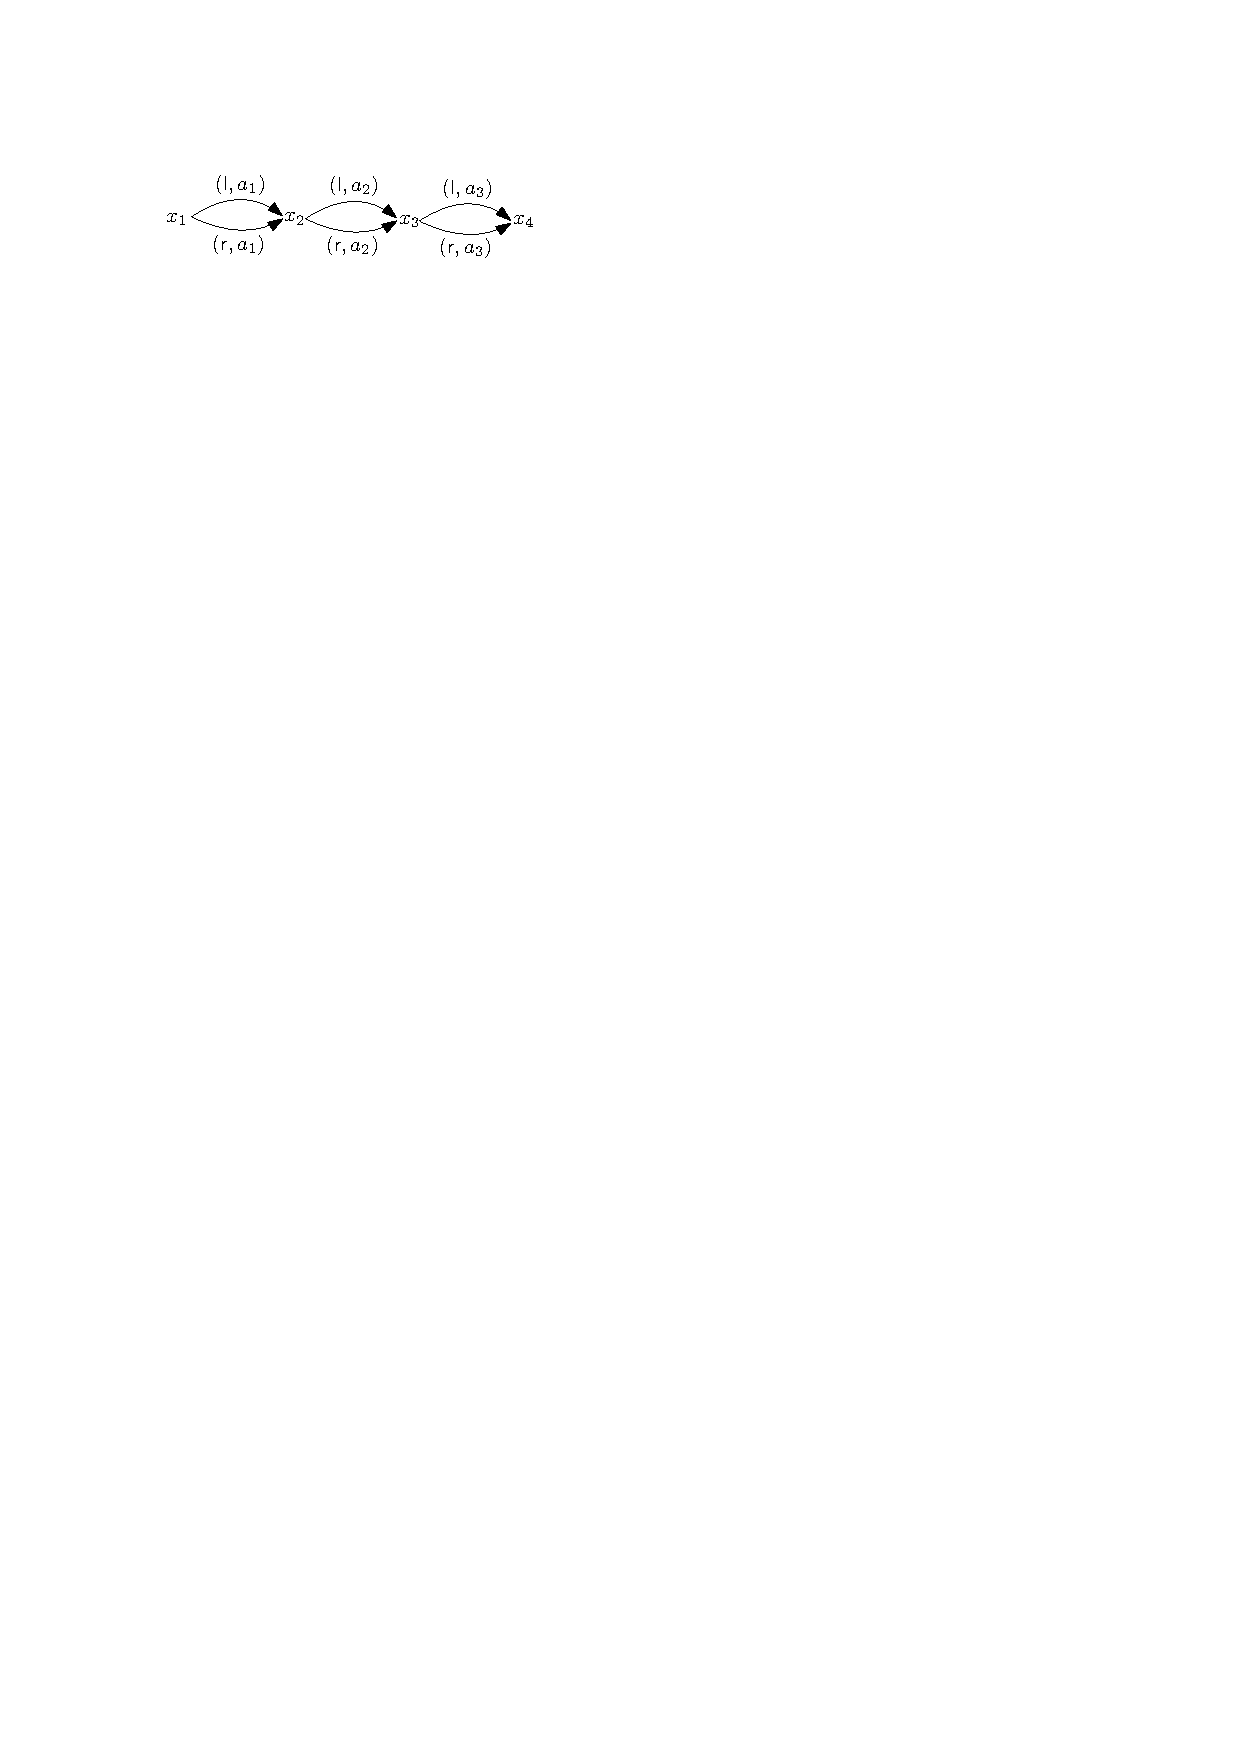
\includegraphics[scale=0.7]{dmdidx-example.pdf}
\end{center}
\caption{The diamond index  and the number of paths in $G_C$}\label{fig-dmdidx-exmp}
\end{figure}
\end{example}

In Section~\ref{sec:replaceallsl}--\ref{sec:replaceallre}, we will apply a refined analysis of the complexity of the decision procedures for proving Theorem~\ref{thm-main} and get the following results.

\begin{corollary}\label{cor-pspace}
The satisfiability problem is PSPACE-complete for the following fragments of $\strline[\replaceall]$:
\begin{itemize}
\item the single-letter case, plus the condition that the diamond indices of the dependency graphs are bounded by a constant $c$, 
%
\item the constant-string case, plus the condition that the $\rpleft$-lengths of the dependency graphs are bounded by a constant $c$, 

%
\item the regular-expression case, plus the condition that the $\rpleft$-lengths of the dependency graphs are at most $1$.
\end{itemize}
\end{corollary}

Corollary~\ref{cor-pspace} partially justifies our choice to present the decision procedures for the single-letter, constant-string, and regular-expression case separately. Intuitively, when the pattern parameters of $\replaceall$ terms become less restrictive, the decision procedures become more involved, and more constraints should be put on the dependency graphs in order to achieve the PSPACE upper bound. The PSPACE lower bound follows from the observation that the nonemptiness of the intersection of the regular expressions $e_1, \cdots, e_n$ over the alphabet $\{0,1\}$, which is a PSPACE-complete problem, can be reduced to the satisfiability of the formula $y = \replaceall((a b)^n, a, x) \wedge x \in (0+1)^\ast \wedge y \in e_1 \circ b  \circ \cdots \circ b \circ e_n$ (where $a, b \not \in \{0,1\}$), which belongs to all fragments in Corollary~\ref{cor-pspace}.\zhilin{Remark for the pspace lower bound, please check.}

%The proof of Theorem~\ref{thm-main} utilises a concept of dependency graphs defined below.



%Therefore,  in the following, without loss of generality, we assume that 
%in each $\strline[\replaceall]$ constraint $C=\varphi \wedge \psi$, the concatenation symbol $\concat$ does not occur in $\varphi$. 
 



%!TEX root = popl2018.tex


\section{Decision procedure for $\strline[\replaceall]$: The single-letter case} \label{sec:replaceallsl}





%%%%%%%%%%%%%%%%%%%%%%%%%%%%%%%%%
%%%%%%%%%%%%%%%%%%%%%%%%%%%%%%%%%
\hide{
\subsection{Encode concatenation by replaceall}

We will transform a given constraint $\varphi$ into a constraint $\varphi'$ which is concatenation free. As the first step, we extend the original alphabet with two fresh letters $a,b$.

For each $x=yz$, we introduce a new variable $x'$ and replace $x=yz$ by two new constraints
$x'=\replaceall(ab, a, x)$ and $x=\replaceall(x', b, z)$.

\begin{proposition}
	$\varphi$ and $\varphi'$ are equisatisfiable.
\end{proposition}
}
%%%%%%%%%%%%%%%%%%%%%%%%%%%%%%%%%
%%%%%%%%%%%%%%%%%%%%%%%%%%%%%%%%%


%\subsection{The single-letter case}

In this section, we consider the single-letter case, that is, for the $\strline[\replaceall]$ formula $C = \varphi \wedge \psi$, every term of the form $\replaceall(z, e, z')$ in $\varphi$ satisfies that $e=a$ for $a \in \Sigma$.
We begin by explaining the idea of the decision procedure in the case where there is a single use of a $\replaceall(\cdots)$ term.
Then we describe the decision procedure in full.

%We first assume that the regular constraint $\psi = \bigwedge \limits_{x \in \vars(\varphi)} x \in e_x$, that is, there is exactly one atomic regular constraint for each variable.

%We first explain the basic idea of the decision procedure.

\subsection{A single use of $\replaceall(\cdots)$}

Let us start with the simple situation that
\[C \equiv x = \replaceall(y, a, z) \wedge x \in e_1 \wedge y \in e_2 \wedge z \in e_3,\]
where, for $i =1, 2, 3$, suppose  $\cA_i = (Q_i, \delta_i, q_{0,i}, F_i)$
%\cA_y = (Q_y, \delta_y, q_{0, y}, F_y), \cA_z = (Q_z, \delta_z, q_{0, z}, F_z)$
is the NFA corresponding to $e_i$.

From the semantics, $C$ is satisfiable if and only if $x, y, z$ can be assigned with strings $u, v, w$ so that: (1) $u$ is obtained from $v$ by replacing all the occurrences of $a$ in $v$ with $w$, and (2) $u, v, w$ are accepted by $\cA_1, \cA_2, \cA_3$ respectively. Let $u,v,w$ be the strings satisfying these two constraints. As $u$ is accepted by $\cA_1$,  there must be an accepting run of $\cA_1$ on $u$. Let $v = v_1 a v_2 a \cdots a v_k$ such that for each $i \in [k]$, $v_i \in (\Sigma \setminus \{a\})^*$. Then $u = v_1 w v_2 w \cdots w v_k$ and there are states $q_1, q'_1, \cdots, q_{k-1}, q'_{k-1}, q_k$  such that
%
$$
q_{0,1} \xrightarrow[\cA_1]{v_1} q_1 \xrightarrow[\cA_1]{w} q'_1 \xrightarrow[\cA_1]{v_2} q_2 \xrightarrow[\cA_1]{w} q'_2 \cdots q_{k-1} \xrightarrow[\cA_1]{w} q'_{k-1} \xrightarrow[\cA_1]{v_k} q_k
$$
%
 and $q_k \in F_{1}$. Let $T_z$ denote $\left\{(q_i, q'_i) \mid i \in [k-1] \right\}$. Then $w \in \Ll(\cA_3)\ \cap\ \bigcap \limits_{(q, q') \in T_z} \Ll(\cA_1(q, q'))$. In addition, let  $\cB_{\cA_1,a,T_z}$ be the NFA obtained from $\cA_1$ by removing all the $a$-transitions first and then adding the $a$-transitions $(q, a, q')$ for $(q, q') \in T_z$. Then
 %
$$
q_{0,1} \xrightarrow[\cB_{\cA_1,a,T_z}]{v_1} q_1 \xrightarrow[\cB_{\cA_1,a,T_z}]{a} q'_1 \xrightarrow[\cB_{\cA_1,a,T_z}]{v_2} q_2 \xrightarrow[\cB_{\cA_1,a,T_z}]{a} q'_2 \cdots q_{k-1} \xrightarrow[\cB_{\cA_1,a,T_z}]{a} q'_{k-1} \xrightarrow[\cB_{\cA_1,a,T_z}]{v_k} q_k.
$$
%
Therefore,
$v \in \Ll(\cA_2) \cap \Ll(\cB_{\cA_1,a,T_z})$. We deduce that there is $T_z \subseteq Q_1 \times Q_1$ such that $\Ll(\cA_3)\ \cap\ \bigcap \limits_{(q, q') \in T_z} \Ll(\cA_1(q, q')) \neq \emptyset$ and $ \Ll(\cA_2) \cap \Ll(\cB_{\cA_1,a,T_z}) \neq \emptyset$. In addition, it is not hard to see that this condition is also sufficient for the satisfiability of $C$. The arguments proceed as follows: Let $v \in  \Ll(\cA_2) \cap \Ll(\cB_{\cA_1,a,T_z})$ and $w \in \Ll(\cA_3)\ \cap\ \bigcap \limits_{(q, q') \in T_z} \Ll(\cA_1(q, q'))$. From $v \in \Ll(\cB_{\cA_1,a,T_z})$, we know that there is an accepting run of $\cB_{\cA_1,a,T_z}$ on $v$. Recall that $\cB_{\cA_1,a,T_z}$ is obtained from $\cA_1$ by first removing all the $a$-transitions, then adding all the transitions $(q,a,q')$ for $(q,q') \in T_z$.  Suppose $v = v_1 a v_2 \cdots a v_k$ such that $v_i \in (\Sigma \setminus \{a\})^*$ for each $i \in [k]$ and
$$
q_{0,1} \xrightarrow[\cB_{\cA_1,a,T_z}]{v_1} q_1 \xrightarrow[\cB_{\cA_1,a,T_z}]{a} q'_1 \xrightarrow[\cB_{\cA_1,a,T_z}]{v_2} q_2 \xrightarrow[\cB_{\cA_1,a,T_z}]{a} q'_2 \cdots q_{k-1} \xrightarrow[\cB_{\cA_1,a,T_z}]{a} q'_{k-1} \xrightarrow[\cB_{\cA_1,a,T_z}]{v_k} q_k
$$
is an accepting run of $\cB_{\cA_1,a,T_z}$ on $v$. Then $q_{0,1} \xrightarrow[\cA_1]{v_1} q_1$, and for each $i \in [k-1]$ we have $(q_i, q'_i) \in T_z$ and $q'_i \xrightarrow[\cA_1]{v_{i+1}} q'_{i+1}$; moreover, $q_k \in F_1$.
Let $u = \replaceall(v, a, w)=v_1 w v_2 \cdots w v_k$. Since $w \in \bigcap \limits_{(q, q') \in T_z} \Ll(\cA_1(q, q'))$,  we infer that
$$
q_{0,1} \xrightarrow[\cA_1]{v_1} q_1 \xrightarrow[\cA_1]{w} q'_1 \xrightarrow[\cA_1]{v_2} q_2 \xrightarrow[\cA_1]{w} q'_2 \cdots q_{k-1} \xrightarrow[\cA_1]{w} q'_{k-1} \xrightarrow[\cA_1]{v_k} q_k
$$
is an accepting run of $\cA_1$ on $u$. Therefore, $u$ is accepted by $\cA_1$ and $C$ is satisfiable.

\begin{proposition}\label{prop-sat-sl-case}
Let $C \equiv x = \replaceall(y, a, z) \wedge x \in e_1 \wedge y \in e_2 \wedge z \in e_3$. Then $C$ is satisfiable iff there is a set $T_{z} \subseteq Q_1 \times Q_1$ such that $\Ll(\cA_3)\ \cap\ \bigcap \limits_{(q, q') \in T_z} \Ll(\cA_1(q, q')) \neq \emptyset$ and $ \Ll(\cA_2) \cap \Ll(\cB_{\cA_1,a,T_z}) \neq \emptyset$.
\end{proposition}

From Proposition~\ref{prop-sat-sl-case}, we can decide the satisfiability of $C$ in polynomial space as follows:
\begin{description}
\item[Step I.] Guess a set $T_{z} \subseteq Q_1 \times Q_1$.
%
\item[Step II.] Guess an accepting run of the product automaton of $\cA_3$ and $\cA_1(q, q')$ for $(q,q') \in T_{z}$.
%
\item[Step III.] Guess an accepting run of the product automaton of $\cA_2$ and $\cB_{\cA_1, a,  T_{z}}$.
\end{description}
During Step II and III, it is sufficient to record $T_z$ and a state of the product automaton, which occupies only a polynomial space.

The above decision procedure can be easily generalised to the case that there are multiple atomic regular constraints for $x$. For instance, let $x \in e_{1,1} \wedge x \in e_{1,2}$ and for $j = 1, 2$, $\cA_{1,j} = (Q_{1,j}, \delta_{1, j}, q_{0,1, j}, F_{1,j})$ be
the NFA corresponding to $e_{1,j}$. Then in Step I, two sets $T_{1,z} \subseteq Q_{1,1} \times Q_{1,1}$ and $T_{2,z} \subseteq Q_{1,2} \times Q_{1,2}$ are guessed, moreover, Step II and III are adjusted accordingly.

\begin{example}\label{exmp-sl}
Let $C \equiv x= \replaceall(y, 0, z) \wedge x \in e_1 \wedge y \in e_2 \wedge z \in e_3$, where $e_1=(0+1)^* (00(0+1)^* + 11(0+1)^*)$,  $e_2= (01)^*$,  and $e_3 = (10)^*$. The NFA $\cA_{1}, \cA_{2}, \cA_{3}$ corresponding to $e_1, e_2, e_3$ respectively are illustrated in Figure~\ref{fig-sl-exmp}. Let $T_z = \{(q_0, q_0), (q_1, q_2)\}$.  Then
$$
\begin{array}{l c l}
 \Ll(\cA_3)\ \cap\ \bigcap \limits_{(q, q') \in T_z} \Ll(\cA_1(q, q'))  & = & \Ll(\cA_3)\ \cap \Ll(\cA_1(q_0, q_0)) \cap \Ll(\cA_1(q_1,q_2)) \\
& = & \Ll((10)^*) \cap \Ll((0+1)^*) \cap \Ll(1(0+1)^*) \\
& \neq & \emptyset.
\end{array}
$$
In addition, $\cB_{\cA_1, 0, T_z}$ (also illustrated in Figure~\ref{fig-sl-exmp}) is obtained from $\cA_1$ by removing all the $0$-transitions, then adding the transitions $(q_0, 0, q_0)$ and $(q_1, 0, q_2)$. Then
$$
 \Ll(\cA_2) \cap \Ll(\cB_{\cA_1,0,T_z})   =  (01)^* \cap (0+1)^* 10 1^* \neq \emptyset.
$$
Therefore, we can choose $z$ to be a string from $\Ll(\cA_3) \cap \ \bigcap \limits_{(q, q') \in T_z} \Ll(\cA_1(q, q'))=\Ll((10)^*) \cap \Ll((0+1)^*) \cap \Ll(1(0+1)^*)$, say $10$, and $y$ to be a string from $ \Ll(\cA_2) \cap \Ll(\cB_{\cA_1,0,T_z})   =  (01)^* \cap (0+1)^* 10 1^*$, say $0101$,  then $x$ gets the value $\replaceall(0101, 0, 10)=101101$, which is in $\Ll(\cA_1)$. Therefore, $C$ is satisfiable.\qed
%
\begin{figure}[htbp]
\begin{center}
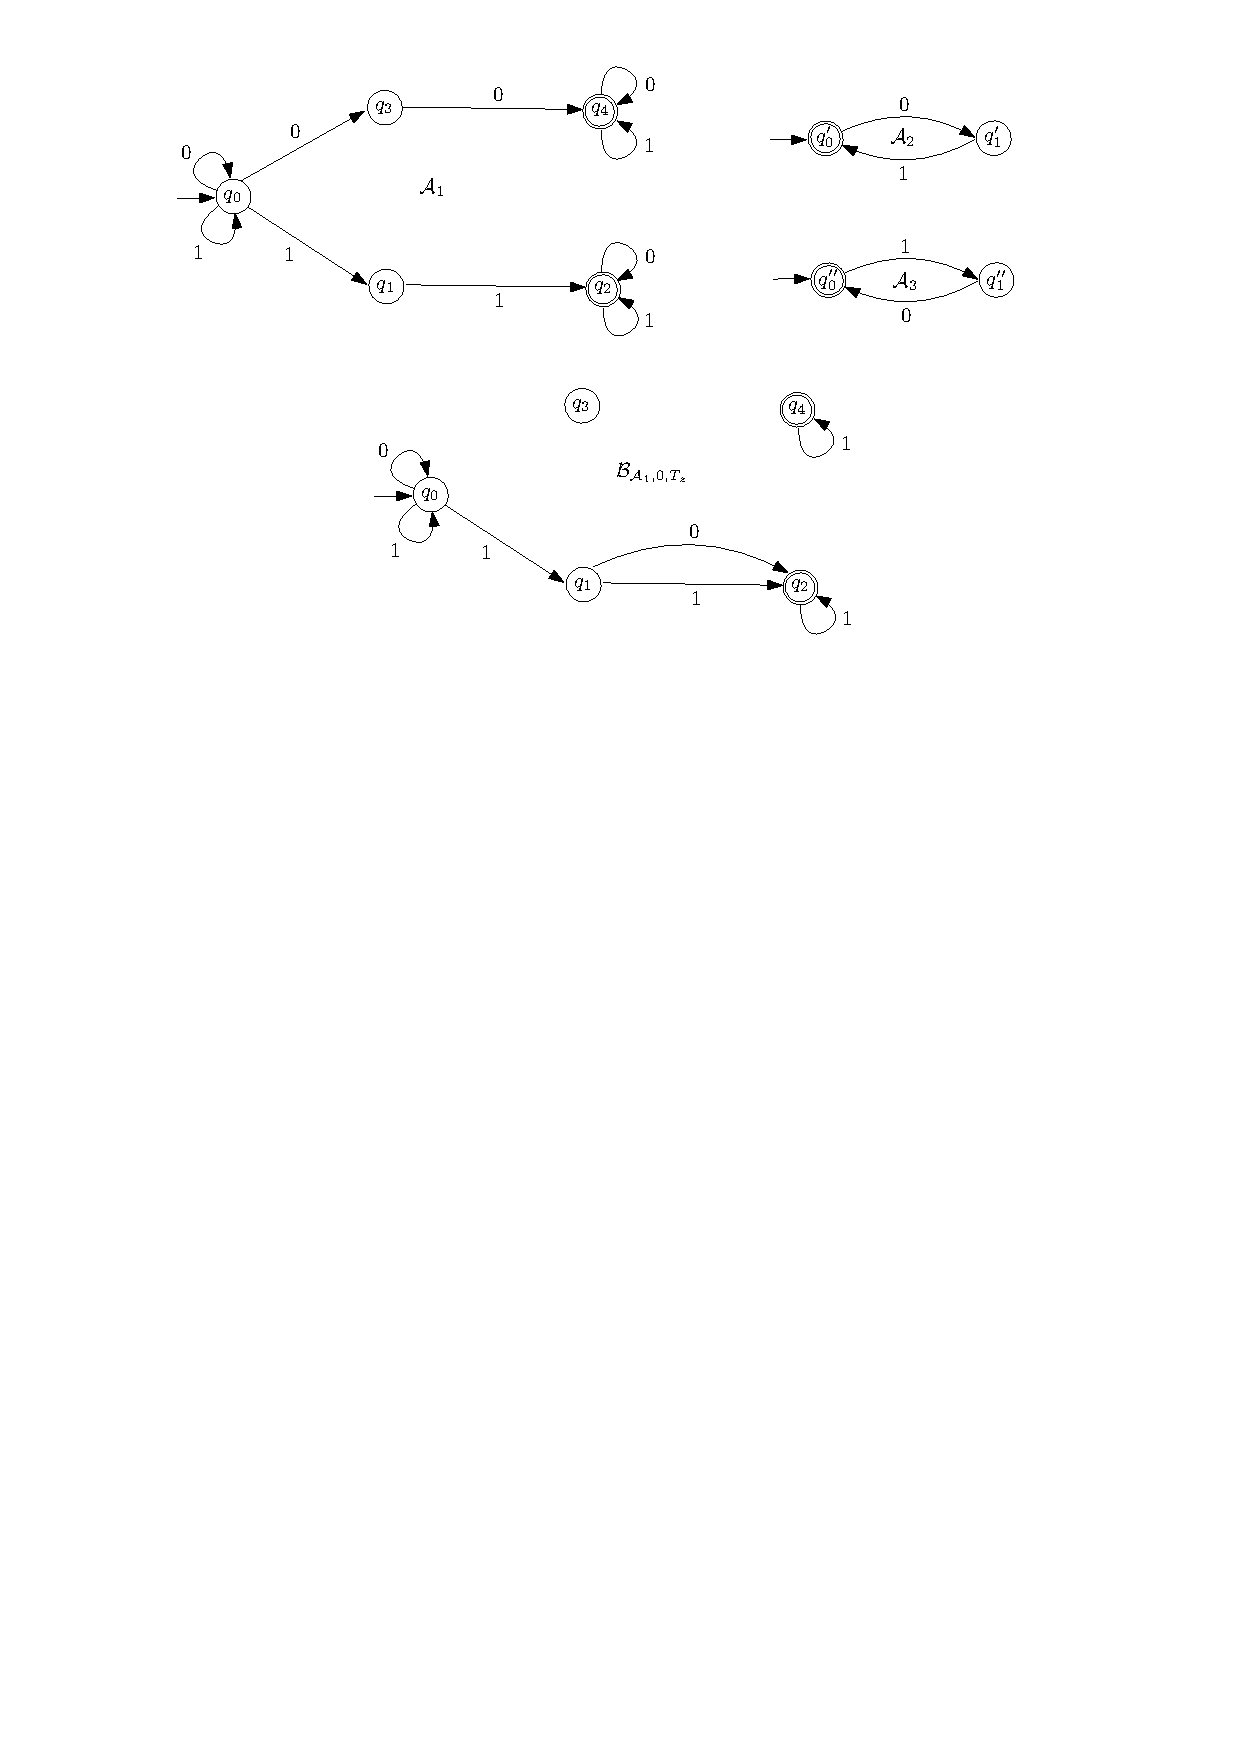
\includegraphics[scale=0.8]{single-letter-example.pdf}
\end{center}
\caption{An example for the single-letter case: One $\replaceall$}\label{fig-sl-exmp}
\end{figure}
\end{example}


\subsection{The general case}

Let us now consider the general case where $C$ contains multiple occurrences of $\replaceall(\cdots)$ terms.
Then the satisfiability of $C$ is decided by the following two-step procedure.

\smallskip

\noindent{\bf Step I.} We utilise the dependency graph $C$ and compute nondeterministically a collection of atomic regular constraints $\cE(x)$ for each variable $x$, in a top-down manner.

%During the computation, for each variable $x$, the collection of atomic regular constraints
Notice that $\cE(x)$ is represented succinctly as a set of pairs $(\cT, \cP)$, where $\cT=(Q, \delta)$ is a transition graph and $\cP \subseteq Q \times Q$. The intention of $(\cT, \cP)$ is to represent succinctly the collection of the atomic regular constraints containing $(Q, \delta, q, \{q'\})$ for each $(q,q') \in \cP$, where $q$ is the initial state and $\{q'\}$ is the set of final states.

%\tl{you want to say that all regular constraints $\cE(x)$ share the same "underlying" graph, but differ in the initial and final states.} \tl{I rephrased a bit-- the original was commented below. Check whether this is what you mean}

Initially, let $G_0:= G_C$.  In addition, for each variable $x$ with the conjunct $x \in e$ in $\psi$ we define $\cE_0(x)$ as follows.  Let $\cA=(Q, \delta, q_0, F)$ be the NFA corresponding to $e$. We nondeterministically choose $q \in F$ and set $\cE_0(x):=  \{((Q, \delta), \{(q_0, q)\})\}$.


%In addition, for each variable $x$, compute $\cE_0(x)$ as follows: Initially, let $\cE_0(x) := \emptyset$.
%For each conjunct $x \in e$ in $\psi$, let $\cA=(Q, \delta, q_0, F)$ be the NFA corresponding to $e$, then nondeterministically choose $q \in F$ and let $\cE_0(x):= \cE_0(x) \cup \{((Q, \delta), \{(q_0, q)\})\}$.
%

We begin with $i:= 0$ and repeat the following procedure until we reach some $i$ where $G_i$ is an empty graph, i.e. a graph without edges.
Note that $G_0$ was defined above.
\begin{enumerate}
\item Select a vertex $x$ of $G_i$ such that $x$ has no predecessors \tl{parent} and has two successors in $G_i$. Suppose $(x, (\rpleft, a), y)$ and $(x, (\rpright,a), z)$ are the two edges out of $x$ in $G_i$ and $\cE_i(x)=\{(\cT_1,\cP_1), \cdots, (\cT_k, \cP_k)\}$, where for each $j \in [k]$, $\cT_j = (Q_j, \delta_j)$. Then $\cE_{i+1}(z)$ and  $\cE_{i+1}(y)$ and $G_{i+1}$ are computed as follows:
\begin{enumerate}
\item For each $j \in [k]$, guess a set $T_{j, z} \subseteq Q_j \times Q_j$.
%
\item If $y \neq z$, then let
$$\cE_{i+1}(z):= \cE_{i}(z) \cup \left\{(\cT_j, T_{j,z}) \mid j \in [k] \right\}$$
and
$$\cE_{i+1}(y): = \cE_{i}(y) \cup \left\{(\cT_{\cT_j, a, T_{j,z}}, \cP_j) \mid j \in [k] \right\},$$
where $\cT_{\cT_j, a, T_{j,z}}$ is obtained from $\cT_j$ by first removing all the $a$-transitions, then adding all the transitions $(q, a, q')$ for $(q,q') \in T_{j,z}$.

Otherwise, let
$$\cE_{i+1}(z):= \cE_{i}(z) \cup \left\{(\cT_j, T_{j,z}) \mid j \in [k] \right\} \cup \left\{(\cT_{\cT_j, a, T_{j,z}}, \cP_j) \mid j \in [k] \right\}.$$
In addition, for each vertex $x'$ distinct from $x, y, z$, let $\cE_{i+1}(x') := \cE_i(x')$.
We set $\cE_{i+1}(x) = \emptyset$.
%
\item Let $G_{i+1}:= G_i \setminus \{(x, (\rpleft, a), y), (x, (\rpright,a), z)\}$.
\end{enumerate}
%
\item Let $i: = i+1$.
\end{enumerate}

For each variable $x$, let $\cE(x)$ denote the set $\cE_i(x)$ after exiting the above loop.

\smallskip

\noindent {\bf Step II.}
For each source variable $x$, guess an accepting run of the product automaton of all the NFA in $\cE(x)$.

\smallskip

%Note that in the first sight, the cardinalities of the sets $\cE(x)$ seem exponential w.r.t. the size of $C$ in the worst case and the nondeterministic algorithm may take exponential space.
%By a refined analysis, we can see that the cardinalities of the sets $\cE(x)$ are in fact polynomial.

It remains to argue the correctness and complexity of the above procedure.
Correctness follows a similar argument to Proposition~\ref{prop-sat-sl-case} and is presented at the end of this section.
We first give an example then argue the complexity.

\begin{example}
Suppose $C \equiv x= \replaceall(y, 0, z) \wedge y = \replaceall(y', 1, z') \wedge x \in e_1 \wedge y \in e_2 \wedge z \in e_3 \wedge y' \in e_4  \wedge z' \in e_5$, where $e_1, e_2, e_3$ are as in Example~\ref{exmp-sl}, $e_4=0^* 1^* 0^* 1^*$, and $e_5=0^*1^*$. Let $\cA_4,\cA_5$ be the NFA corresponding to $e_4$ and $e_5$ respectively (see Figure~\ref{fig-sl-exmp-nested}). The dependency graph $G_C$ of $C$ is illustrated in Figure~\ref{fig-sl-exmp-nested}. Let $\cT_1,\cdots, \cT_5$ be the transition graph of $\cA_1,\cdots, \cA_5$ respectively. Then the collection of regular constraints $\cE(\cdot)$ are computed as follows.
\begin{itemize}
\item Let $G_0=G_C$. We nondeterministically choose $\cE_0(x) = \{(\cT_1, \{(q_0, q_2)\})\}$, $\cE_0(y) = \{(\cT_2, \{(q^\prime_0, q^\prime_0)\})\}$, $\cE_0(z) = \{(\cT_3, \{(q^{\prime\prime}_0, q^{\prime\prime}_0)\})\}$, $\cE_0(y^\prime) = \{(\cT_4, \{(p_0, p_1)\})\}$, $\cE_0(z^\prime) = \{(\cT_5, \{(p^{\prime}_0, p^{\prime}_1)\})\}$.
%
\item Select the vertex $x$ in $G_0$, construct $\cE_1(y)$ and $\cE_1(z)$ as in Example~\ref{exmp-sl}, that is, nondeterministically choose $T_z =\{(q_0, q_0), (q_1,q_2)\}$, let $\cE_1(z) = \{(\cT_3, \{(q^{\prime\prime}_0, q^{\prime\prime}_0)\}), (\cT_1, \{(q_0,q_0), (q_1, q_2)\})\}$ and $\cE_1(y)=\{(\cT_2, \{(q^\prime_0, q^\prime_0)\}), (\cT_{\cT_1, 0, T_z}, \{(q_0,q_2)\})\}$, where $\cT_{\cT_1, 0, T_z}$ is the transition graph of $\cB_{\cA_1, 0, T_z}$ illustrated in Figure~\ref{fig-sl-exmp}. In addition, $\cE_1(x)=\cE_0(x)$, $\cE_1(y')=\cE_0(y')$ and $\cE_1(z')=\cE_0(z')$. Finally, $G_1$ is obtained from $G_0$ by removing the two edges out of $x$.
%
\item Select the vertex $y$ in $G_1$, construct $\cE_2(y')$ and $\cE_2(z')$ as follows: Nondeterministically choose $T_{1,z'} = \{(q^\prime_0, q^\prime_0)\}$  for $\cT_2$ and $T_{2,z'}=\{(q_0,q_1),(q_1,q_2)\}$ for $\cT_{\cT_1, 0, T_z}$, let
$$\cE_2(z')=\left\{(\cT_5, \{(p^{\prime}_0, p^{\prime}_1)\}), (\cT_2, \{(q^\prime_0, q^\prime_0)\}), (\cT_{\cT_1, 0, T_z}, \{(q_0,q_1),(q_1,q_2)\}) \right\},$$
and
$$\cE_2(y')=\left\{ (\cT_4, \{(p_0, p_1)\}), (\cT_{\cT_2, 1, T_{1,z'}}, \{(q^\prime_0, q^\prime_0)\}), (\cT_{\cT_{\cT_1, 0, T_z}, 1, T_{2,z'}}, \{(q_0,q_2)\}) \right\},$$
where $\cT_{\cT_2, 1, T_{1,z'}}$ and $\cT_{\cT_{\cT_1, 0, T_z}, 1, T_{2,z'}}$ are illustrated in Figure~\ref{fig-sl-exmp-nested-2}. In addition, $\cE_2(x)=\cE_1(x)$, $\cE_2(y)=\cE_1(y)$, and $\cE_2(z)=\cE_1(z)$. Finally, $G_2$ is obtained from $G_1$ by removing the two edges out of $y$.
%
\end{itemize}
Since $G_2$ contains no edges, we have $\cE(x)=\cE_2(x)$, similarly for $\cE(y)$, $\cE(z)$, $\cE(y')$, and $\cE(z')$.
For the three source variables $y', z', z$, it is not hard to check that $01$ belongs to the intersection of the regular constraints in $\cE(z')$, $11$ belongs to the intersection of the regular constraints in $\cE(y')$, and $10$ belongs to the intersection of the regular constraints in $\cE(z)$. Then $y$ takes the value $\replaceall(11, 1, 01)=0101 \in \Ll(e_2)$, and $x$ takes the value $\replaceall(0101, 0, 10)=101101 \in \Ll(e_1)$. Therefore, $C$ is satisfiable. \qed
\begin{figure}[htbp]
\begin{center}
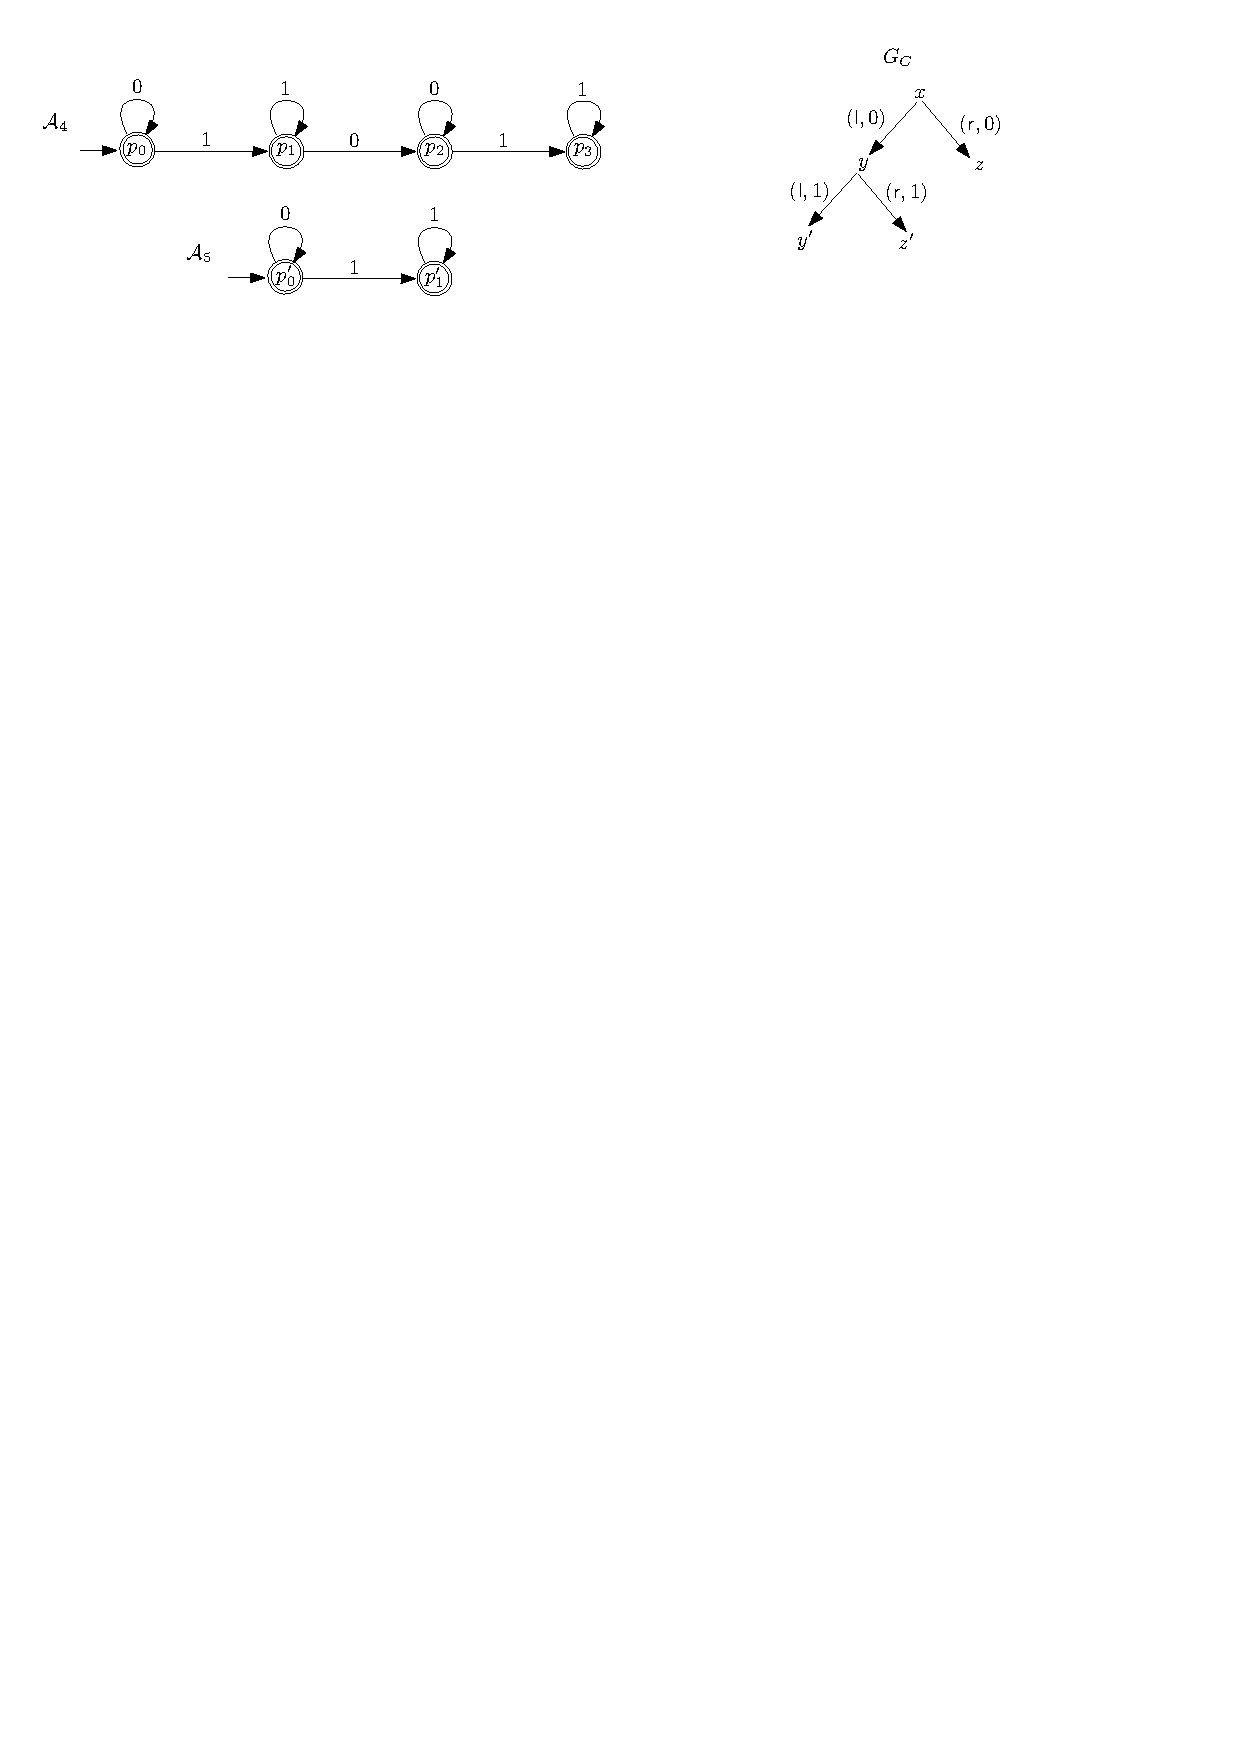
\includegraphics[scale=0.8]{single-letter-example-nested.pdf}
\end{center}
\caption{An example for the single-letter case: Multiple $\replaceall$}\label{fig-sl-exmp-nested}
\end{figure}

\begin{figure}[htbp]
\begin{center}
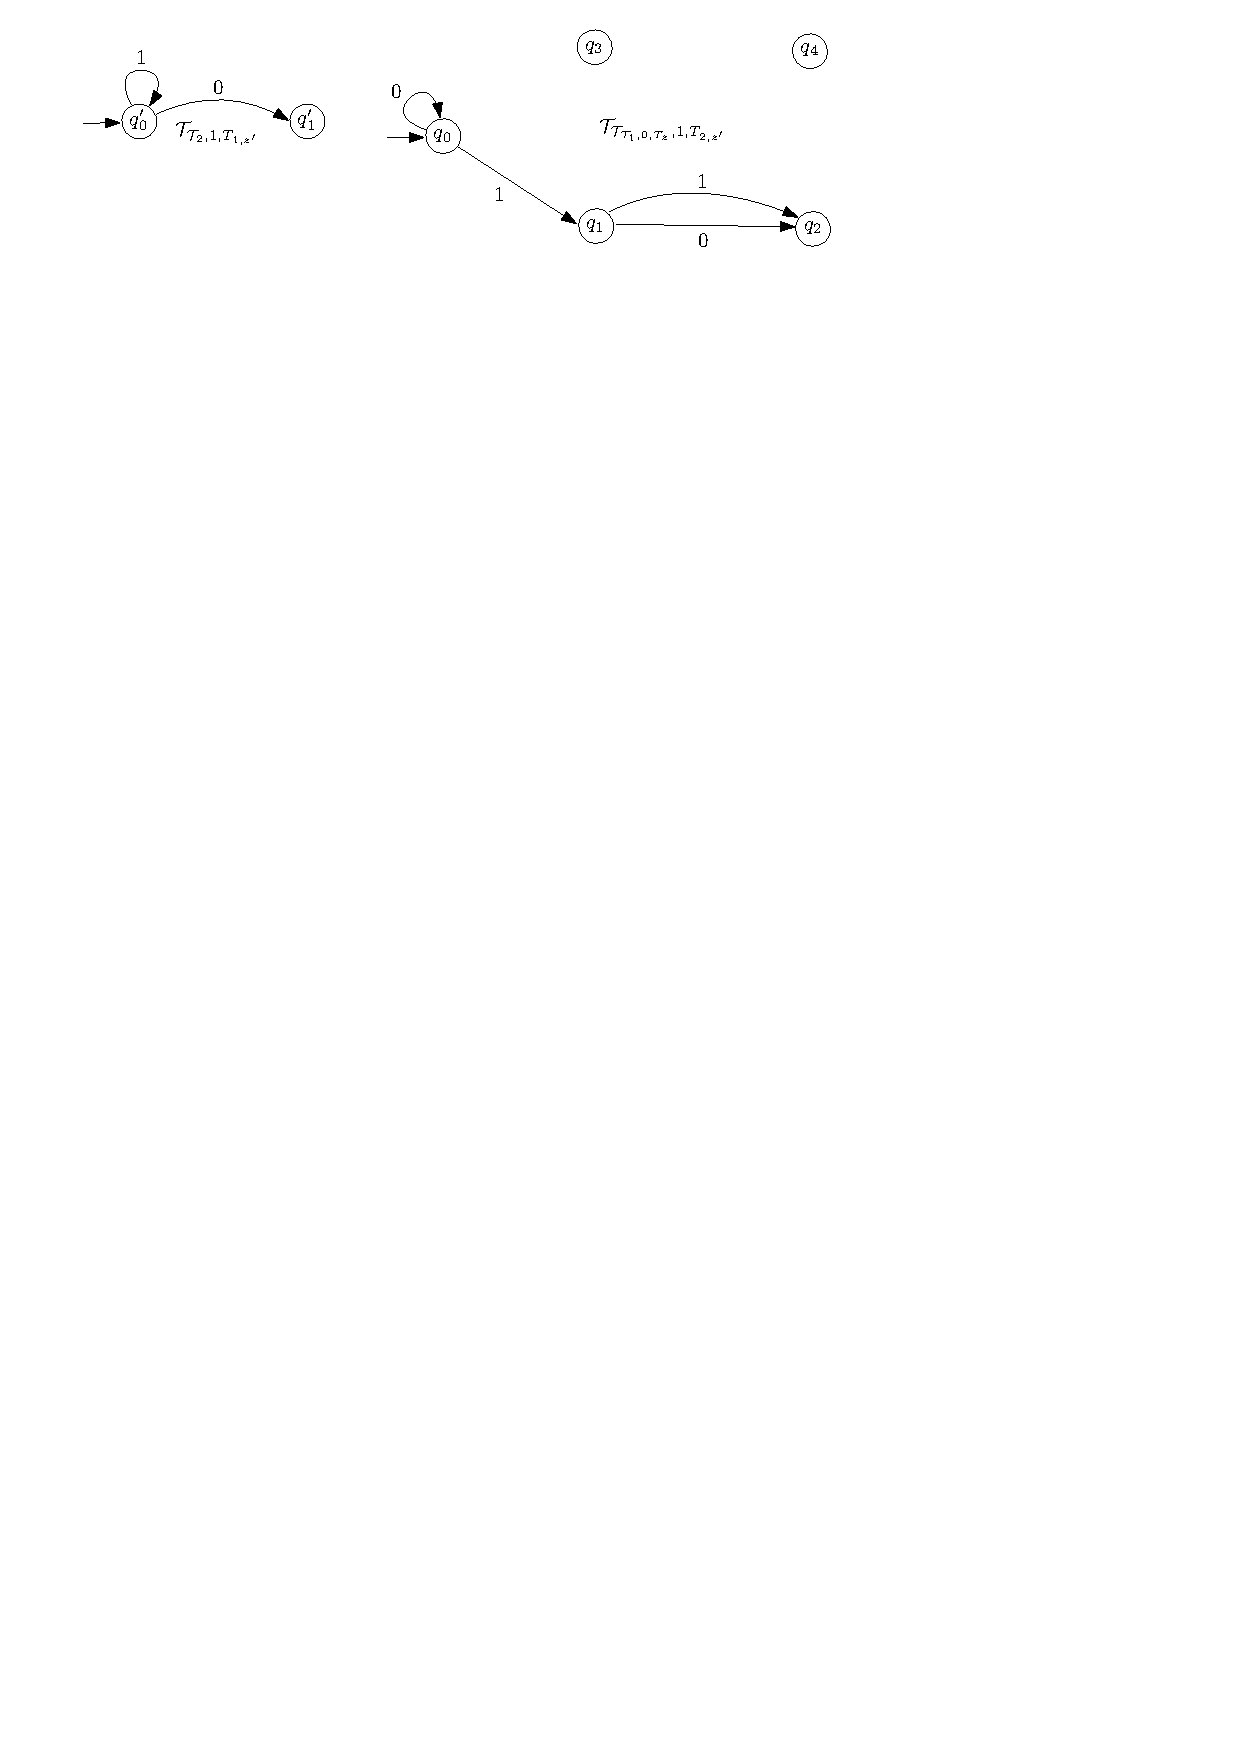
\includegraphics[scale=0.8]{single-letter-example-nested-2.pdf}
\end{center}
\caption{$\cT_{\cT_2, 1, T_{1,z'}}$ and $\cT_{\cT_{\cT_1, 0, T_z}, 1, T_{2,z'}}$}\label{fig-sl-exmp-nested-2}
\end{figure}
\end{example}




\subsubsection{Complexity}

To show that the aforementioned nondeterministic decision procedure works in exponential space, it is sufficient to show that the cardinalities of the sets $\cE(x)$ are exponential w.r.t. the size of $C$.

\begin{proposition}
The cardinalities of $\cE(x)$ for the variables $x$ in $G_C$ are at most exponential  in the size of $C$ and become polynomial for $\strline_{\sf ss}[\replaceall]$ formulae.
\end{proposition}

\begin{proof}
%The transition graphs $\cT=(Q, \delta)$ and $\cT'=(Q', \delta')$ are said to be \emph{isomorphic} if there is a bijection $\pi: Q \rightarrow Q'$ such that for each $q, q' \in Q$ and $a \in \Sigma$, $(q, a, q') \in \delta$ iff $(\pi(q), a, \pi(q')) \in \delta'$.
%
Let $K$ denote the maximum cardinality of $\cE_0(x)$ for vertices $x$ in $G_C$.
%In addition, for each node $x$ in $G_C$, let $\#^{\sf anc}$
%In addition, let $M$ denote the maximum size (number of states) of the NFA in $\cE_0(x)$ for nodes $x$ in $G_C$.
For each $i$ and each vertex $x$ in $G_C$, let  $\#^{\sf anc}_i(x)$ denote the number of ancestors of $x$ in $G_i$.
%, in addition, let ${\sf Idx}^{\sf arb}_i(x)$ denote the maximum number of join vertices in a path starting from $x$ in $G_i$.

%the number of edges of $G_0 \setminus G_i$ (i.e. the subgraph of $G_0$ comprising all the edges not in $G_i$) that are co-reachable from $x$ in  $G_0 \setminus G_i$.

% and $\#_{\sf lft}(x)$ denote the number of $\rpleft$-edges that are co-reachable from $x$ in $G_C$.

%Then the proposition follows from the following claim, since for each node $x$, $|\cE(x)| \le |\cG(\cE(x))|M^2$.

We first prove the following claim.

\smallskip

\noindent {\bf Claim}. For each $i$ and each vertex $x$ in $G_C$,
$|\cE_i(x)| \le 3^i K$. In addition, if $C \in \strline_{\sf ss}[\replaceall]$, then for each non-source variable $x$ in $G_C$, $|\cE_i(x)| \le (\#^{\sf anc}_0(x)-\#^{\sf anc}_i(x)+1) K$.
%In addition, if $G_C$ is a tree, then $|\cE_i(x)| \le (\#^{\sf anc}_0(x)-\#^{\sf anc}_i(x)+1) K$.

\smallskip

We prove the claim by an induction on $i$.

\smallskip


\noindent {\it Induction base}: $i=0$. Evidently $|\cE_0(x)| \le K = 3^0 K$. Moreover, if $C \in \strline_{\sf ss}[\replaceall]$, then for each non-source variable $x$, $|\cE_0(x)| \le K = (\#^{\sf anc}_0(x)-\#^{\sf anc}_0(x)+1) K$.
% = (\#^{\sf anc}_0(x)-\#^{\sf anc}_0(x)+1) K$.

\smallskip

\noindent {\it Induction step}:
Suppose $i > 0$.

Let $x$ be the vertex without predecessors and with successors in $G_{i-1}$ that is used to construct $G_{i}$. In addition, let $(x, (\rpleft, a), y)$ and $(x, (\rpright, a), z)$ be the two edges out of $x$ in $G_{i-1}$.

Let us first assume $y \neq z$.
Then $|\cE_{i}(z)| \le |\cE_{i-1}(z)| + |\cE_{i-1}(x)|$ and $|\cE_{i}(y)| \le |\cE_{i-1}(y)| + |\cE_{i-1}(x)|$.  By the induction hypothesis, $|\cE_{i-1}(x)| \le  3^{i-1} K$, $|\cE_{i-1}(y)| \le 3^{i-1} K$, and $|\cE_{i-1}(z)| \le 3^{i-1} K$. Therefore, $|\cE_{i}(z)|  \le |\cE_{i-1}(z)| + |\cE_{i-1}(x)| \le 3^{i-1} K + 3^{i-1} K \le 3^i K$. Similarly, $|\cE_{i}(y)| \le 3^i K$.

Next, we assume $y = z$. Then $|\cE_{i}(z)| \le |\cE_{i-1}(z)| + |\cE_{i-1}(x)| + |\cE_{i-1}(x)| \le 3* 3^{i-1} K = 3^i K$.

Let us assume that $C \in \strline_{\sf ss}[\replaceall]$, moreover, either $y$ or $z$ is not a source variable. Then $y \neq z$. Because otherwise, the in-degree of $y=z$ in $G_C$ is more than one, from the fact that $G_C$ is source-sharing, we deduce that $y=z$ has to be a source variable, a contradiction. Let us first assume that $z$ is not a source variable. Then the in-degree of $z$ is one, that is, the edge from $x$ to $z$ is the only incoming edge of $z$ in $G_C$. From this, we deduce that  $\cE_{i-1}(z) = \cE_0(z)$. Therefore, $|\cE_{i}(z)| \le |\cE_{i-1}(z)| + |\cE_{i-1}(x)| \le K + |\cE_{i-1}(x)|$. By the induction hypothesis, $|\cE_{i-1}(x)| \le (\#^{\sf anc}_{0}(x) - \#^{\sf anc}_{i-1}(x)+1)K$. We deduce that $|\cE_{i}(z)| \le K+ (\#^{\sf anc}_{0}(x) - \#^{\sf anc}_{i-1}(x)+1)K$. Moreover, since $\#^{\sf anc}_{0}(z) = \#^{\sf anc}_{0}(x)+1$ and $\#^{\sf anc}_{i-1}(x)=\#^{\sf anc}_{i}(x)= \#^{\sf anc}_{i}(z)=0$, we have $|\cE_{i}(z)| \le K+ (\#^{\sf anc}_{0}(z)-1 - \#^{\sf anc}_{i}(z)+1)K = (\#^{\sf anc}_{0}(z) - \#^{\sf anc}_{i}(z)+1)K$.
Similarly, if $y$ is not a source variable, we have $|\cE_{i}(y)| \le |\cE_{i-1}(y)| + |\cE_{i-1}(x)| = |\cE_{0}(y)| + |\cE_{i-1}(x)| \le K+|\cE_{i-1}(x)| \le K+ (\#^{\sf anc}_{0}(x) - \#^{\sf anc}_{i-1}(x)+1)K \le K+ (\#^{\sf anc}_{0}(y)-1 - \#^{\sf anc}_{i}(y)+1)K = (\#^{\sf anc}_{0}(y) - \#^{\sf anc}_{i}(y)+1)K$.

The proof of the claim is complete.

To complete the proof of the proposition, let $H$ be the maximum length of the paths in $G_C$. From the claim, we deduce that for each non-source variable $x$, $|\cE(x)| \le (H-1)K$. In addition, for each source variable $y$ in $G_C$, suppose that the in-degree of $y$ in $G_C$ is $m$, then $|\cE(y)| \le K + \sum \limits_{x: \mbox{ \small predecessor of } y} |\cE(x)| \le  K+m(H-1)K=(mH-m+1) K$.
%
Therefore, we conclude that if $C \in \strline_{\sf ss}[\replaceall]$, then the cardinalities of $\cE(x)$ become polynomial in the size of $C$.
\end{proof}

%\begin{quote}
%\it Let $x$ be a node in the graph without predecessors and $x = \replaceall(y, a, z)$ be a conjunct of $\varphi$ and $\cA_1, \dots, \cA_m$ be a collection of regular constraints for $x$. Then remove the two edges out of $x$, guess $T_{i, z} \subseteq Q_i \times Q_i$ for $i \in [m]$, and add additional regular constraints to $y$ and $z$ as specified above.
%\end{quote}

%For doing this, we need deal with the typical situation that $x = \replaceall(y, a, z)$  and the regular constraints for $x$ are specified by

%We first introduce a concept of dependency graphs.


\subsubsection{Correctness}

Finally, we argue that the above procedure is correct.
Note that Proposition~\ref{prop-sat-sl-case} removed a single $\replaceall(\cdots)$ to obtain only regular constraints.
Each step of our decision procedure effectively eliminates a $\replaceall(\cdots)$.
Similar to Proposition~\ref{prop-sat-sl-case}, each step maintains satisfiability from the preceding step.

In more detail, from each $G_i$ we can define a constraint $C_i$.
This constraint is a conjunction of the following clauses.
For each variable $x$ such that $\cE_i(x)$ is not empty, we let $e_i(x)$ be the regular expresion equivalent to the conjunction of all constraints in $\cE_i(x)$.
Since this is the conjunction of multiple NFAs, it is regular.
We assert in $C_i$ that $x \in e_i(x)$.
Next, for each vertex $x$ such that $(x, (\rpleft, a), y)$ and $(x, (\rpright,a), z)$ are edges in $G_i$, we assert $x = \replaceall(y, a, z)$.

It is immediate that $C_0$ is equivalent to $C$.
We require the following proposition, which gives us correctness of the decision procedure by induction.
Note that the final $C_i$ will be a conjunction of regular constraints on the source variables.

\begin{proposition}
    The constraint $C_i$ is equisatisfiable with $C_{i+1}$.
\end{proposition}

We can see the above proposition by observing that, in each step, $C_i$ is of the form
\[
    x = \replaceall(y, a, z) \wedge x \in e_i(x) \wedge y \in e_i(y) \wedge z \in e_i(z) \wedge C'
\]
where $C'$ does not contain $x$, and $C_{i+1}$ is of the form.
\[
    x = y \in e_{i+1}(y) \wedge z \in e_{i+1}(z) \wedge C' \ .
\]
Note that $C'$ remains unchanged since only one pair of edges were removed from $G_i$ and $\cE_{i+1}(x') = \cE_i(x')$ for all $x'$ distinct from $x$, $y$, and $z$.
First assume $y \neq z$.
Supposing $C_i$ is satisfiable, an argument similar to that of Proposition~\ref{prop-sat-sl-case} shows that the same values of $y$ and $z$ also satisfy $e_{i+1}(y)$ and $e_{i+1}(z)$.
Since $C'$ is unchanged, all $x'$ distinct from $x$, $y$, and $z$ can also keep the same value.
Thus, $C_{i+1}$ is also satisfiable.
In the other direction, take a satisfying assignment to $C_{i+1}$.
From the assignment to $y$ and $z$ we obtain as in Proposition~\ref{prop-sat-sl-case} an assignment to $x$ that satisfies $\replaceall(y, a, z) \wedge x \in e_i(x)$.
Furthermore, the assignments for $y$ and $z$ also satisfy $e_i(y)$ and $e_i(z)$ since $\cE_i(y)$ and $\cE_i(z)$ are subsets of $\cE_{i+1}(y)$ and $\cE_{i+1}(z)$.
Finally, since $C'$ is unchanged, the assignments to all other variables also transfer, giving us a satisfying assignment to $C_i$ as required.
In the case where $y = z$, the argument proceeds analogously to the case $y \neq z$.


%!TEX root = popl2018.tex

\section{Decision procedure for $\strline[\replaceall]$: The constant-string case}\label{sec:replaceallcs}

In this section, we consider the constant-string special case, that is, for an $\strline[\replaceall]$ formula $C = \varphi \wedge \psi$, every term of the form $\replaceall(z, e, z')$ in $\varphi$ satisfies that $e=u$ for $u \in \Sigma^+$. Note that the case when $u=\epsilon$ will be dealt with in Section~\ref{sec:replaceallre}. 

Again, let us start with the simple situation that
$C \equiv x = \replaceall(y, u, z) \wedge x \in e_1 \wedge y \in e_2 \wedge z \in e_3$,
where $|u| \ge 2$. For $i=1,2,3$, let $\cA_i = (Q_i, \delta_i, q_{0, i}, F_i)$
be the NFA corresponding to $e_i$. In addition, let $k = |u|$ and $u = a_1 \cdots a_k$ with $a_i \in \Sigma$ for each $i \in [k]$.

From the semantics, $C$ is satisfiable iff $x, y, z$ can be assigned with  strings $v, w, w'$ such that: (1) $v = \replaceall(w, u, w')$, and (2) $v,w, w'$ are accepted by $\cA_1, \cA_2, \cA_3$ respectively. Let $v, w, w'$ be the strings satisfying these two constraints. Since $v = \replaceall(w, u, w')$, we know that there are strings $w_1, w_2, \cdots, w_n$ such that $w= w_1 u w_2 \cdots u w_n$ and $v = w_1 w' w_2 \cdots w' w_n$. As $v$ is accepted by $\cA_1$, there is an accepting run of $\cA_1$ on $v$, say
$$
q_{0,1} \xrightarrow[\cA_1]{w_1} q_1 \xrightarrow[\cA_1]{w'} q'_1 \xrightarrow[\cA_1]{w_2} q_2 \xrightarrow[\cA_1]{w'} q'_2 \cdots q_{n-1} \xrightarrow[\cA_1]{w'} q'_{n-1} \xrightarrow[\cA_1]{w_n} q_n.
$$
Let $T_z = \{(q_i, q'_i) \mid i \in [n]\}$. Then $w' \in \Ll(\cA_3) \cap\ \bigcap \limits_{(q,q') \in T_z} \Ll(\cA_1(q, q'))$. Therefore, $\Ll(\cA_3) \cap\ \bigcap \limits_{(q,q') \in T_z} \Ll(\cA_1(q, q')) \neq \emptyset$. Similar to the single-letter case, we construct an NFA $\cB_{\cA_1, u, T_z}$ to characterise the satisfiability of $C$.  More precisely, $C$ is satisfiable iff there is $T_z \subseteq Q_1 \times Q_1$ such that $\Ll(\cA_3) \cap\ \bigcap \limits_{(q,q') \in T_z} \Ll(\cA_1(q, q')) \neq \emptyset$ and
$\Ll(\cA_2) \cap \Ll(\cB_{\cA_1, u, T_z}) \neq \emptyset$. Intuitively, when reading the string $w$, $\cB_{\cA_1, u, T_z}$ simulates the generation of $v$ from $w$ and $w'$ (that is, the replacement of  every occurrence of $u$ in $w$ with $w'$) and verifies that $v$ is accepted by $\cA_1$, by using $T_z$.
To build $\cB_{\cA_1, u, T_z}$, we utilise the concepts of window profiles and parsing automata defined below.
%
%Intuitively, the window profiles encode the matching of the suffixes of a string of length $|u|$ w.r.t. the prefixes of $u$ and a parsing automaton for $u$ uses window profiles of $u$ to pinpoint the first, second, \dots, occurrence of $u$ in a string.


%Let us start with the simple case that $C \equiv x = \replaceall(y, u, z) \wedge \bigwedge \limits_{i \in [k]} x \in e_{i}$ such that $|u| \ge 2$.  In addition, for $i \in [k]$, suppose $\cA_i = (Q_i, \delta_i, q_{0, i}, F_i)$
%is the NFA corresponding to $e_i$.
%\begin{enumerate}
%\item For each $i \in [k]$, we will guess a set $T_{i, z} \subseteq Q_i \times Q_i$, which intuitively means that in $\cA_i$, for each state pair $(q, q') \in T_{i, z}$, starting from $q$, after reading $z$, the state $q' $ can be reached. The functions $(T_{i, z})_{i \in [k]}$ induce regular constraints $\Ll(\cA_i(q,q'))$ on $z$, where $i \in [k]$ and $(q,q') \in T_{i, z}$.
%
%\item For each $i \in [k]$, we construct an NFA $\cB_{\cA_i, u,  T_{i, z}}$, which specifies some additional regular constraint on $y$. Intuitively, a string $v$ is accepted by $\cB_{\cA_i, u,  T_{i, z}}$ iff either $v \not \in \Sigma^\ast u \Sigma^\ast$ and $v$ is accepted by $\cA_i$, or otherwise, let $v = v'_1 u v'_2 u \dots v'_{k-1} u v'_{k}$ such that $v'_i u' \not \in \Sigma^\ast u \Sigma^\ast$ for each $i \in [k-1]$ and each strict prefix $u'$ of $u$ and $v'_k \not \in \Sigma^\ast u \Sigma^\ast$, then $q_{i,0} \xrightarrow{v'_1} q_1 \xrightarrow{T_{i,z}} q'_1 \xrightarrow{v'_2} q_2 \xrightarrow{T_{i,z}} q'_2 \dots \xrightarrow{v'_{k-1}} q_{k-1} \xrightarrow{T_{i,z}} q'_{k-1} \xrightarrow{v'_k} q_k$ for states $q_1, q'_1, \dots, q_{k-1}, q'_{k-1}, q_k \in Q_i$ with $q_k \in F_{i,z}$.
%\end{enumerate}
%
%In order to construct the NFA $\cB_{\cA_i, u,  T_{i, z}}$, we introduce concepts of window profiles and parsing automata defined below.
%
%Let $u \in \Sigma^+$ and $k=|u| \ge 2$.


\begin{definition}[window profiles w.r.t. $u$]\zhilin{I changed the notation from $k$-window profile to window profile, and $\wprof_{u,k}$ to $\wprof_u$. Please check whether there are still occurrences of the old notation below.}
Let $v$ be a nonempty string with $k=|v|$, and $i \in [k]$. Then the \emph{window profile of the position $i$ in $v$ w.r.t. $u$} is $\overrightarrow{W}  \in \{\bot,\top\}^{k-1}$ defined as follows:
\begin{itemize}
\item If $i \ge k-1$, then for each $j \in [k-1]$, $\overrightarrow{W}[j] = \top$ iff $v[i-j+1] \cdots v[i]=u[1] \cdots u[j]$.
%
\item If $i < k-1$, then for each $j \in [i]$, $\overrightarrow{W}[j] = \top$ iff $v[i-j+1] \cdots v[i]=u[1] \cdots u[j]$, and for each $j: i < j \le k-1$, $\overrightarrow{W}[j] = \bot$.
\end{itemize}
Let $\wprof_{u}$ denote the set of window profiles of the positions in nonempty strings w.r.t. $u$.
\end{definition}

%Intuitively, in a position $i$ of a string $v$, the $k$-window profile $\overrightarrow{W}$ of $i$ in $v$ w.r.t. $u$ is an abstraction of the substring $v[i-k+2] \dots v[i]$ such that for each $j \in [k-1]$, $\overrightarrow{W}[j] = \top$ iff $v[i-j+1] \dots v[i] = u[1] \dots u[j]$.

\begin{proposition}
$|\wprof_{u}| \le |u|$.
\end{proposition}
%
\begin{proof}
%The arguments for this fact proceed as follows: 
Let $k=|u|$. For each profile $\overrightarrow{W}$, let $v$ be a nonempty string and $i$ be a position of $v$ such that for each $j \in [k-1]$, $\overrightarrow{W}[j] = \top$ iff $v[i-j+1] \dots v[i] = u[1] \dots u[j]$. Define ${\sf idx}_{\overrightarrow{W}}$ as follows: If there is $j \in [k-1]$ such that $\overrightarrow{W}[j]=\top$, then ${\sf idx}_{\overrightarrow{W}}$ is the maximum of such indices $j \in [k-1]$, otherwise, ${\sf idx}_{\overrightarrow{W}} =0$. The following fact holds for $\overrightarrow{W}$ and ${\sf idx}_{\overrightarrow{W}}$: 
\begin{itemize}
	\item for each $j': {\sf idx}_{\overrightarrow{W}} < j' \le k-1$, $\overrightarrow{W}[j']=\bot$,
	\item in addition, since $v[i-{\sf idx}_{\overrightarrow{W}}+1] \cdots v[i] = u[1] \cdots u[{\sf idx}_{\overrightarrow{W}}]$, the values of $\overrightarrow{W}[1],\cdots, \overrightarrow{W}[{\sf idx}_{\overrightarrow{W}}]$ are completely determined by $u[1] \cdots u[{\sf idx}_{\overrightarrow{W}}]$.
\end{itemize}
Let $\eta: \wprof_{u} \rightarrow \{0\} \cup [k-1]$ be a function such that for each $\overrightarrow{W} \in \wprof_{u}$, $\eta(\overrightarrow{W})={\sf idx}_{\overrightarrow{W}}$. Then $\eta$ is an injective function, since for every $\overrightarrow{W}, \overrightarrow{W'} \in \wprof_{u}$, ${\sf idx}_{\overrightarrow{W}}  = {\sf idx}_{\overrightarrow{W'}}$ iff $\overrightarrow{W} = \overrightarrow{W'}$. Therefore, we conclude that  $ |\wprof_{u}| \le k$.
\end{proof}

\begin{example}\label{wprof-exmp}
Let $\Sigma = \{0,1\}$, $u = 010$. Then $\wprof_{u}=\{\bot\bot, \top\bot, \bot\top\}$.
\begin{itemize}
\item Consider the string $v=1$ and the position $i=1$ in $v$. Since $v[1]=1 \neq u[1]=0$, the window profile of $i$ in $v$ w.r.t. $u$ is $\bot \bot$.
\item Consider the string $v=00$ and the position $i=2$ in $v$. Since $v[2]=u[1]$ and $v[1]v[2] \neq u[1]u[2]$, the window profile of $i$ in $v$ w.r.t. $u$ is $\top\bot$.
\item Consider the string $v=01$ and the position $i=2$ in $v$. Since $v[2] \neq u[1]$ and $v[1]v[2] = u[1]u[2]$, the window profile of $i$ in $v$ w.r.t. $u$ is $\bot\top$.
\end{itemize}
Note that $\top\top \not \in \wprof_{u}$, since for every string $v$ and the position $i$ in $v$, if $v[i-1]v[i]=u[1]u[2]=01$, then $v[i]=1 \neq 0= u[1]$.
\end{example}

%\mat{Updated the paragraph below to reflect our earlier discussion.}

We will construct a parsing automaton $\cA_u$ from $u$, which parses a string $v$ containing at least one occurrence of $u$ (i.e.\ $v \in \Sigma^\ast u \Sigma^\ast$) into $v_1 u v_2 u \dots v_l u v_{l+1}$ such that $v_j u[1] \dots u[k-1] \not \in \Sigma^\ast u \Sigma^\ast$ for each $1 \le j \le l$.
This ensures that the only occurrence of $u$ in each $v_j u$ is a suffix.
Finally, we also require $v_{l+1} \not \in \Sigma^\ast u \Sigma^\ast$.
The window profiles w.r.t. $u$ will be used to ensure that $v$ is correctly parsed, namely, the first, second, $\cdots$, occurrences of $u$ are correctly identified.

\begin{definition}[Parsing automata]
The \emph{parsing automaton} $\cA_u$ of a string $u$ is the NFA $(Q_u, \delta_u, q_{0,u}, F_u)$ defined as follows.
\begin{itemize}
	\item  $Q_u =\left\{q_0 \right\} \cup \left\{ \left(\search, \overrightarrow{W} \right)\ \big\vert\ \overrightarrow{W} \in \wprof_{u} \right\} \cup  \left\{ \left(\verify, j, \overrightarrow{W} \right) \ \big\vert\ j \in [k-1], \overrightarrow{W} \in \wprof_{u} \right\}$, where $q_0$ is a distinguished state whose purpose will become clear later on,  and the tags ``$\search$" and ``$\verify$" are used to denote whether $\cA_u$ is in the ``search'' mode to search for the next occurrence of $u$, or in the ``verify'' mode to verify that the current position is a part of an occurrence of $u$.
	%
	\item $q_{0,u}=q_0$.

	\item $\delta_{u}$ is defined as follows.
	%guesses over each position, one of the following holds, the substring comprising the next $k$-symbols (including the current one) is $u$ or not.
	\begin{itemize}
		\item The transition $\left(q_0, a, \left(\search, \overrightarrow{W}\right)\right) \in \delta_u$, where $\overrightarrow{W}[1]=\top$ iff $a = u[1]$, and for each $i: 2 \le i \le k-1$, $\overrightarrow{W}[i] = \bot$.
		%
		\item The transition $\left(q_0, u[1], \left(\verify, 1, \overrightarrow{W}\right)\right) \in \delta_u$, where $\overrightarrow{W}[1]=\top$ and for each $i: 2 \le i \le k-1$, $\overrightarrow{W}[i] = \bot$.
%
		\item For each state $\left(\search, \overrightarrow{W} \right)$ and $a \in \Sigma$ such that $\overrightarrow{W}[k-1] = \bot$ or $a \neq u[k]$,
		\begin{itemize}
			\item the transition $\left(\left(\search, \overrightarrow{W} \right), a, \left(\search, \overrightarrow{W'} \right)\right) \in \delta_u$, where $\overrightarrow{W'}[1] = \top$ iff $a = u[1]$, and for each $i: 2 \le i \le k-1$, $\overrightarrow{W'}[i] =\top$ iff ($\overrightarrow{W}[{i-1}] = \top$ and $a = u[i]$),
			%
			\item if $a = u[1]$, then the transition $\left(\left(\search, \overrightarrow{W} \right), a, \left(\verify, 1, \overrightarrow{W'} \right)\right) \in \delta_u$, where $\overrightarrow{W'}[1]=\top$,  and for each $i: 2 \le i \le k-1$, $\overrightarrow{W'}[i] =\top$ iff ($\overrightarrow{W}[{i-1}] = \top$ and $a = u[i]$).
			%
		\end{itemize}
		%
		\item For each state $\left(\verify, i-1, \overrightarrow{W} \right)$ and $a \in \Sigma$ such that
		\begin{itemize}
			\item $2 \le i \le k-1$,
			\item $\overrightarrow{W}[i-1]=\top$, $a = u[i]$, and
			\item either $\overrightarrow{W}[k-1]=\bot$ or $a \neq u[k]$,
		\end{itemize}
		we have $\left(\left(\verify, i-1, \overrightarrow{W} \right), a, \left(\verify, i, \overrightarrow{W'} \right)\right) \in \delta_u$, where for each $j: 2 \le j \le k-1$, $\overrightarrow{W'}[j] = \top$ iff $\overrightarrow{W}[j-1]=\top$ and $a = u[j]$.
		%
		\item For each state $\left(\verify, k-1, \overrightarrow{W} \right)$ and $a \in \Sigma$ such that $\overrightarrow{W}[k-1]=\top$ and $a  = u[k]$, we have $\left(\left(\verify, k-1, \overrightarrow{W} \right), a, q_0\right) \in \delta_u$.
		%where $\bot^k$ in $(\search, \bot^k)$ is used to \emph{reinitialise} the $k$-window profile w.r.t. $u$.
		%
	\end{itemize}
Note that the constraint $\overrightarrow{W}[k-1] = \bot$ or $a \neq u[k]$ is used to guarantee that each occurrence of the state $q_0$, except the first one, witnesses the \emph{first} occurrence of $u$ from the beginning or after its previous occurrence. In other words, the constraint $\overrightarrow{W}[k-1] = \bot$ or $a \neq u[k]$ is used to guarantee that after an occurrence of $q_0$, if $q_0$ has not been reached again,  then $u$ is forbidden to occur.

% parsing a string $v$ into $v_1 u v_2 u \dots v_{l} u v_{l+1}$, we have $v_j u[1] \dots u[k-1] \not \in \Sigma^\ast u \Sigma^\ast$ for each $j \in [l]$, in addition, $v_{l+1} \not \in  \Sigma^\ast u \Sigma^\ast$.
	%
	\item $F_u= \left\{q_0 \right\} \cup \left\{\left(\search, \overrightarrow{W} \right)\ \big\vert\ \overrightarrow{W} \in \wprof_{u} \right\} $. \\
	Note that the states $\left(\verify, j, \overrightarrow{W} \right)$ are not final states, since, when in these states, the verification of the current occurrence of $u$ has not been complete yet.
\end{itemize}
\end{definition}

Let $Q_{\search}  = \left\{ \left(\search, \overrightarrow{W} \right) \ \big\vert\ \overrightarrow{W} \in \wprof_{u} \right\}$,  and $Q_{\verify, i} = \left\{ \left(\verify, i, \overrightarrow{W} \right) \ \big\vert\ \overrightarrow{W} \in \wprof_{u} \right\}$ for each $i \in [k-1]$. In addition, let $Q_{\verify} = \bigcup \limits_{i \in [k-1]} Q_{\verify,i}$.
Suppose $v = v_1 u v_2 u \cdots v_l u v_{l+1}$ such that $v_j u[1] \dots u[k-1] \not \in \Sigma^\ast u \Sigma^\ast$ for each $1 \le j \le l$, in addition, $v_{l+1} \not \in \Sigma^\ast u \Sigma^\ast$. Then there exists a \emph{unique} accepting run $r$ of $\cA_u$ on $v$ such that the state sequence in $r$ is of the form
$q_0\ r_1\ q_0\ r_2\ q_0\ \cdots\ r_l\ q_0\ r_{l+1}$, where for each $j \in [l]$, $r_j \in  \Ll((Q_{\search})^+ \concat Q_{\verify, 1} \concat \cdots  \concat Q_{\verify, k-1})$, and $r_{l+1} \in \Ll((Q_{\search})^*)$. 
%Intuitively, each occurrence of $q_0$, except the first one, witnesses the \emph{first} occurrence of $u$ from the beginning or after its previous occurrence.

%The parsing automaton $\cA_u$ constructed above is \emph{unambiguous} in the sense that for each string $v \in \Sigma^+$, there is \emph{exactly one accepting run} of $\cA_u$ on $v$.

\begin{example}
Consider $u=010$ in Example~\ref{wprof-exmp}. The parsing automaton  $\cA_u$ is illustrated in Figure~\ref{fig-pa-exmp}. Note that there are no $0$-transitions out of $(\search, \bot\top)$, since this would imply an occurrence of $u = 010$, which should be verified by the states from $Q_{\verify}$, more precisely, by the state sequence $q_0 (\verify, 1, \top\bot) (\verify, 2, \bot\top)q_0$.
\begin{figure}[htbp]
\begin{center}
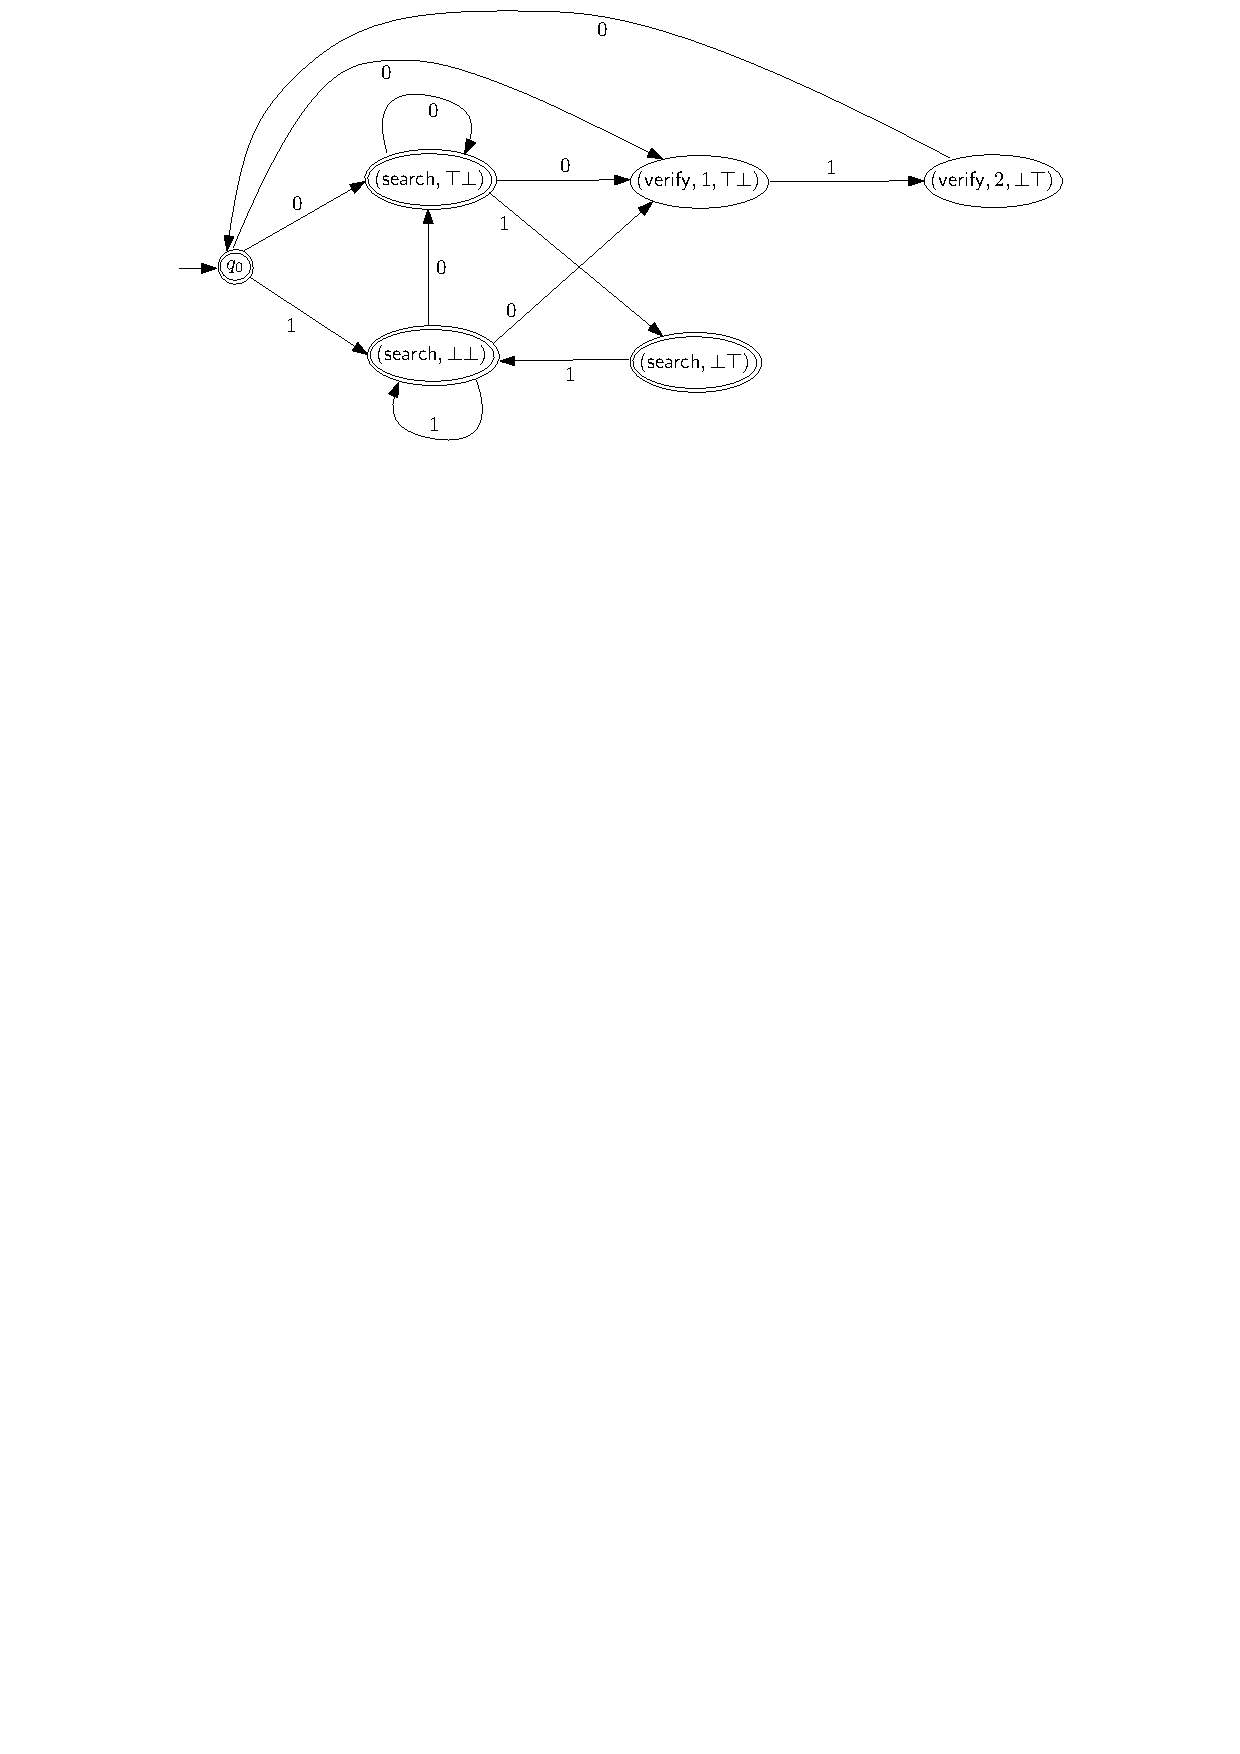
\includegraphics[scale=0.6]{parsing-automata-example.pdf}
\end{center}
\caption{The parsing automaton $\cA_u$ for $u = 010$}\label{fig-pa-exmp}
\end{figure}
\end{example}

We are ready to present the construction of $\cB_{\cA_1, u,  T_{z}}$. The NFA $\cB_{\cA_1, u, T_{z}}$ is constructed by the following three-step procedure.
\begin{enumerate}
\item Construct the product automaton $\cA_1 \times \cA_u$. Note that the initial state of $\cA_1 \times \cA_u$ is $(q_{0},q_0)$ and the set of final states of $\cA_1 \times \cA_u$ is $F_1 \times F_u$.

\item Remove from $\cA_1 \times \cA_u$ all the (incoming or outgoing) transitions associated with the states from $Q_1 \times Q_{\verify}$.

\item For each pair $(q,q') \in T_{z}$ and each sequence of transitions in $\cA_u$ of the form
$$
%\begin{array}{l}
\left(p, u[1], \left(\verify, 1, \overrightarrow{W'_1} \right) \right), \left( \left(\verify, 1, \overrightarrow{W'_1} \right), u[2],
 \left(\verify, 2, \overrightarrow{W'_2}\right) \right), 
 %\\
 %\hspace{3cm} 
 \cdots, \left(\left(\verify, k-1, \overrightarrow{W'_{k-1}} \right), u[k], q_0\right),
%\end{array}
$$
where  $p=q_0$ or $p = \left(\search, \overrightarrow{W} \right)$,
add the following transitions
$$
\begin{array}{c}
\left((q,p), u[1], \left(q, \left(\verify, 1, \overrightarrow{W'_1} \right) \right) \right), 
%\\
\left( \left(q, \left(\verify, 1, \overrightarrow{W'_1} \right) \right), u[2], \left(q, \left(\verify, 2, \overrightarrow{W'_2}\right)\right)\right),  
%\\
\cdots, \\
\left(\left(q, \left(\verify, k-2, \overrightarrow{W'_{k-2}} \right) \right), u[k-1], \left (q, \left (\verify, k-1, \overrightarrow{W'_{k-1}} \right) \right) \right),
%\\ 
\left( \left(q, \left (\verify, k-1, \overrightarrow{W'_{k-1}} \right) \right), u[k], \left(q', q_0 \right)\right).
\end{array}
$$
Note that the number of aforementioned sequences of transitions in $\cA_u$ is at most $|Q_{\search}|+1$, since  $ \overrightarrow{W'_1},\dots,  \overrightarrow{W'_{k-1}}$ are completely determined by $\overrightarrow{W} $ and $u$.
Intuitively, when $\cA_u$ identifies an occurrence of $u$, if the current state of $\cA_1$ is $q$, then after reading the occurrence of $u$, $\cB_{\cA_1, u, T_z}$ jumps from $q$ to some state $q'$ such that $(q,q') \in T_z$.
\end{enumerate}

\begin{example}\label{exmp-cs-case}
Consider $C \equiv x = \replaceall(y, u, z) \wedge x \in e_1 \wedge y \in e_2 \wedge z \in e_3$, where $u = 010$, and $e_1,e_2,e_3$ are as in Example~\ref{exmp-sl} (cf. Figure~\ref{fig-sl-exmp}). 
%The product automaton $\cA_1 \times \cA_u$ is illustrated in Figure~\ref{fig-cs-exmp}, where $\{q_2\} \times \cA_u$ denotes the automaton obtained from $\cA_u$ by changing each state $p$ in $\cA_u$ into $(q_2, p)$, similarly for $\{q_4\} \times \cA_u$. 
Let $T_z = \{(q_0,q_0),(q_1,q_2)\}$. The NFA $\cB_{\cA_1, u, T_z}$ is obtained from the product automaton $\cA_1 \times \cA_u$ (which we give in the appendix for reference) by first removing all the transitions  associated with the states from $Q_1 \times Q_{\verify}$, then adding the transitions according to $T_z$ as aforementioned (see Figure~\ref{fig-cs-exmp-2}, where thick edges indicate added transitions).  It is routine to check that $01010101$ is accepted by $\cB_{\cA_1, u, T_z}$ and $\cA_2$. Moreover, $10 \in \Ll(\cA_3) \cap \Ll(\cA_1(q_0,q_0)) \cap \Ll(\cA_1(q_1,q_2))$. Let $y$ be $01010101$ and $z$ be $10$. Then $x$ takes the value $\replaceall(01010101, 010, 10)=101101$, which is accepted by $\cA_1$. Therefore, $C$ is satisfiable.
%\begin{figure}[htbp]
%\begin{center}
%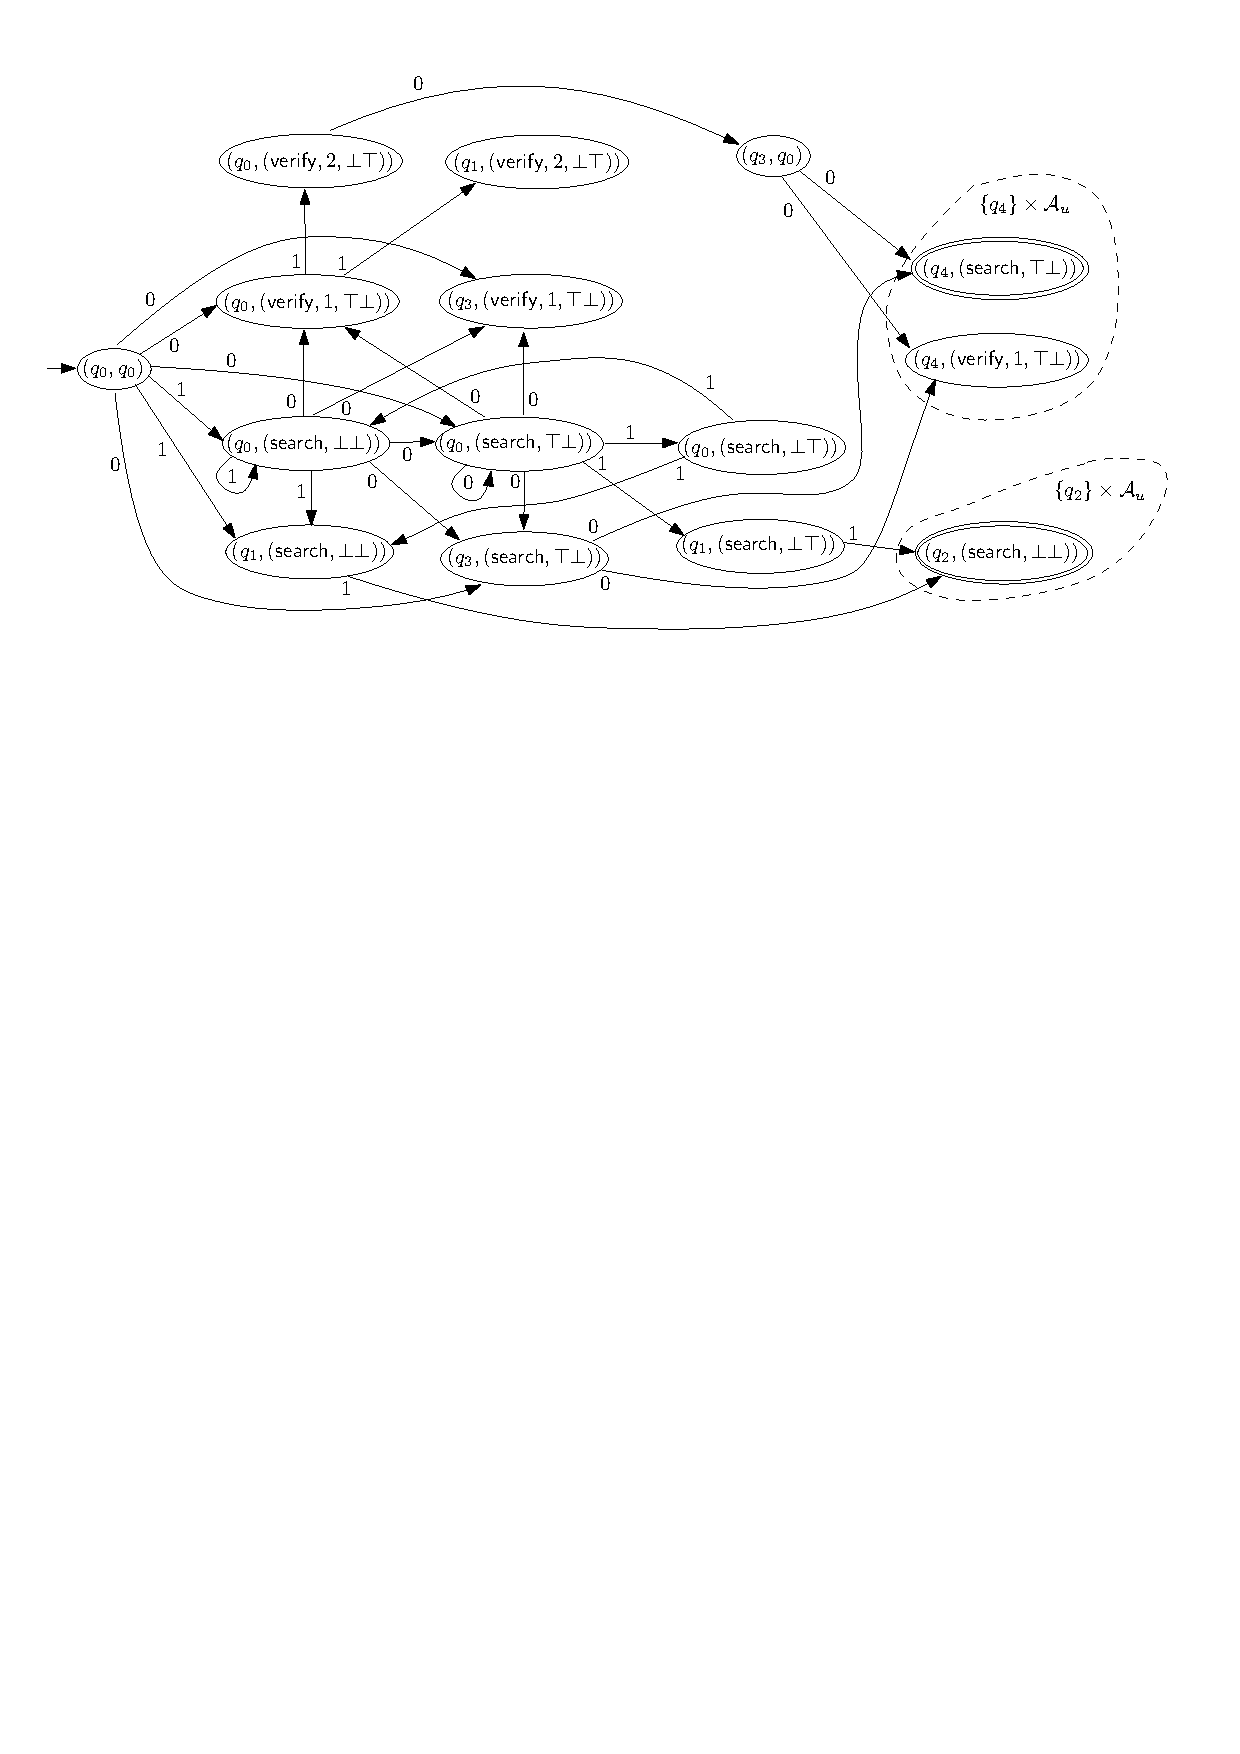
\includegraphics[scale=0.65]{constant-string-example.pdf}
%\end{center}
%\caption{The NFA $\cA_1 \times \cA_u$ for $u = 010$}\label{fig-cs-exmp}
%\end{figure}
%
\begin{figure}[htbp]
\begin{center}
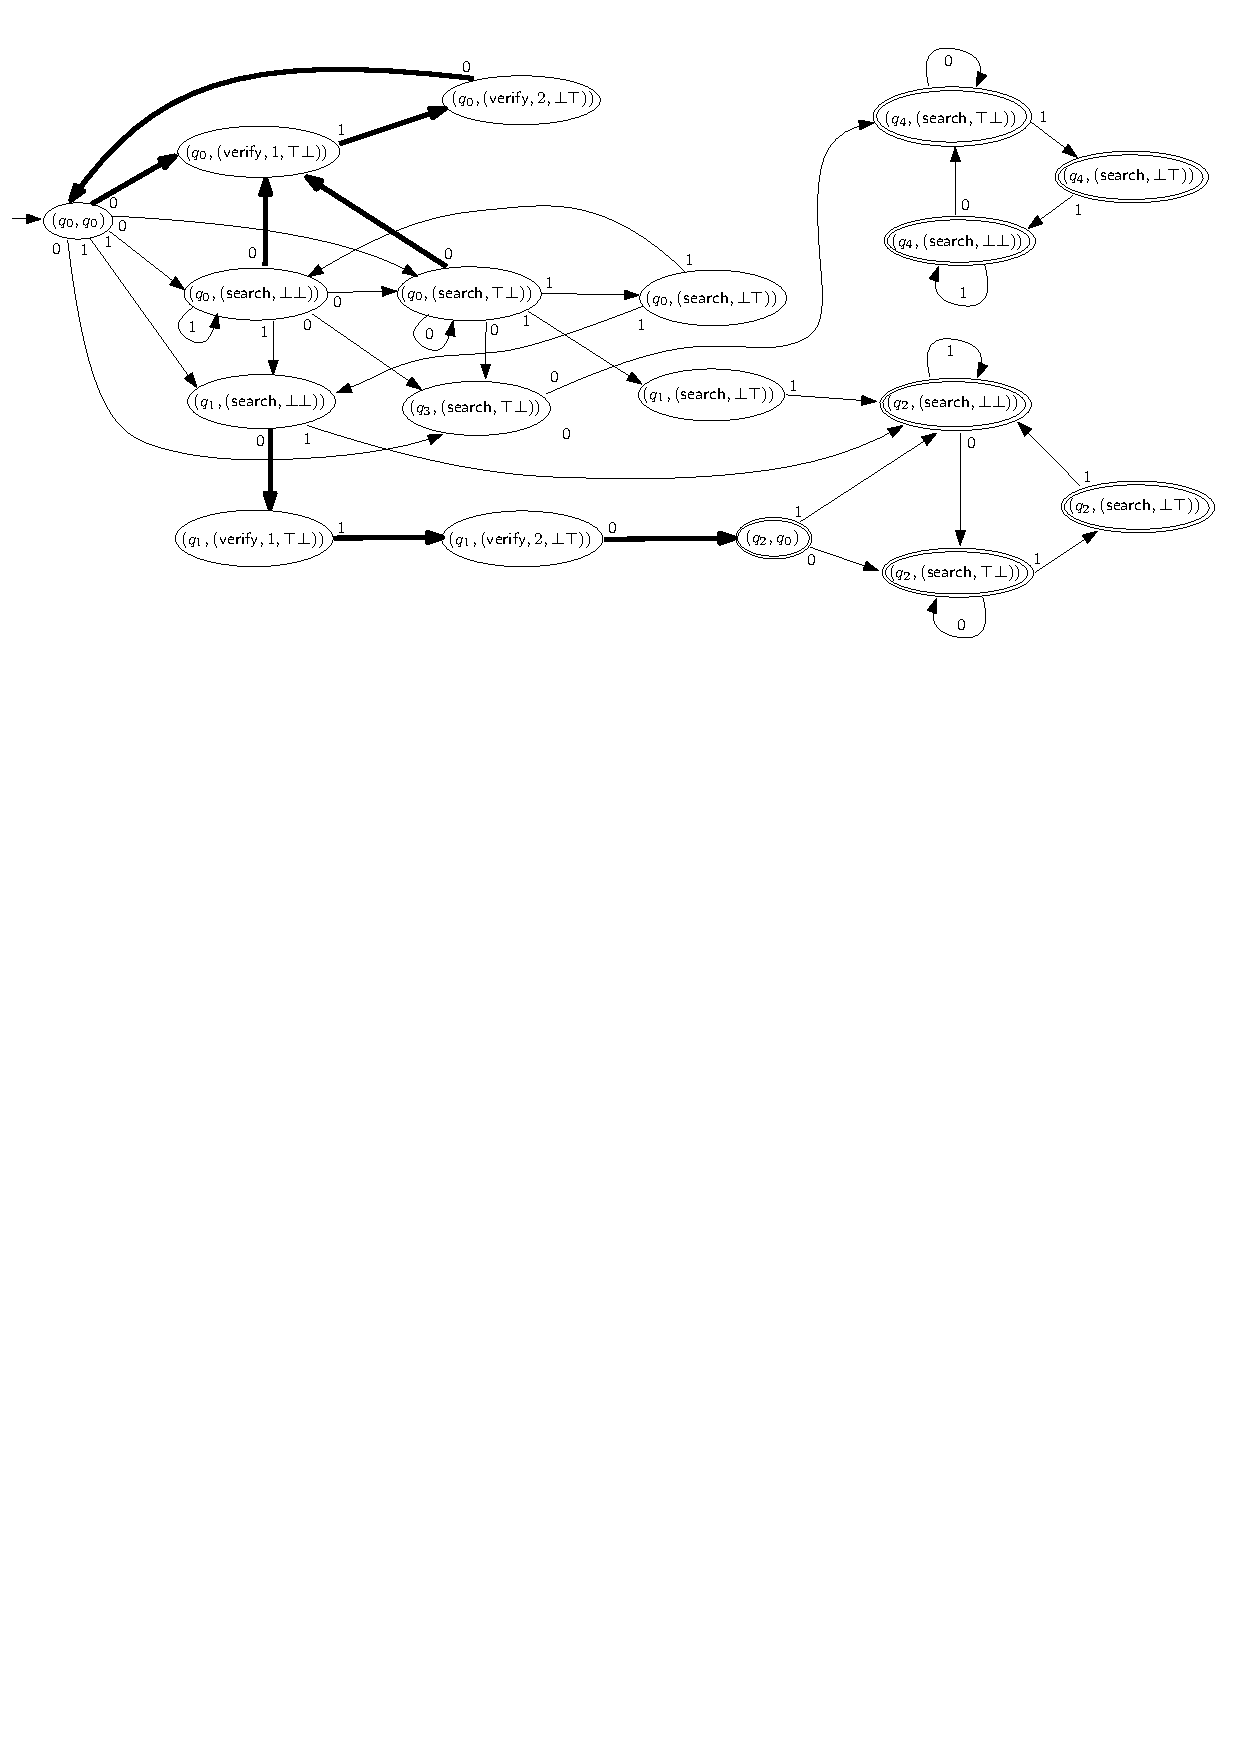
\includegraphics[scale=0.68]{constant-string-example-2.pdf}
\end{center}
\caption{The NFA $\cB_{\cA_1, u, T_z}$ for $u = 010$ and $T_z= \{(q_0,q_0),(q_1,q_2)\}$}\label{fig-cs-exmp-2}
\end{figure}
\end{example}

For the more general case that the $\strline[\replaceall]$ formula $C$ contains more than one occurrence of $\replaceall(-, -, -)$ terms, similar to the single-letter case in Section~\ref{sec:replaceallsl}, we can nondeterministically remove the edges in the dependency graph $G_C$ in a top-down manner and reduce the satisfiability of $C$ to the satisfiability of a collection of regular constraints for source variables.

\paragraph*{Complexity}
When constructing $G_{i+1}$ from $G_i$, suppose the two edges from $x$ to $y$ and $z$ respectively are currently removed, let the labels of the two edges be $({\sf l}, u)$ and $({\sf r}, u)$ respectively. Then each element $(\cT, \cP)$ of $\cE_i(x)$ may be transformed into an element $(\cT', \cP')$ of $\cE_{i+1}(y)$ such that $|\cT'| = O(|u||\cT|)$, meanwhile, it may also be transformed into an element $(\cT'', \cP'')$ of $\cE_{i+1}(z)$ such that $\cT''$ has the same state space as $\cT$. In each step of the decision procedure, the state space of the regular constraints may be multiplied by a factor $|u|$. The state space of these regular constraints is at most exponential in the end, so that we can still solve the nonemptiness problem of the intersection of all these regular constraints in exponential space. In addition, if the $\rpleft$-length of $G_C$ is bounded by a constant $c$, then for each source variable, we get polynomially many regular constraints, where each of them has a state space of polynomial size. Therefore, we can get a polynomial space algorithm. See Appendix~\ref{sec:cs-complexity-full} for a detailed analysis.

%\mat{Also need to say the same about $z$?}\zhilin{the state space of the regular constraint for $z$ is not changed.}

%Similarly to the single-letter case, we can define the dependency graph $G_C$. In addition, we can adapt $\dfs(z, z', a, f)$ into a procedure $\dfs(z, z', u, f)$, which integrates the automata $\cA_{u'}$ into the computation of the functions $f_{z', \cA_z}$, where $u,u'$ are constant strings occurring in the edge-labels in $G_C$.


%!TEX root = popl2018.tex

\section{Decision procedure for $\strline[\replaceall]$: The regular-expression case} \label{sec:replaceallre}

We consider the case that the second parameter of the $\replaceall$ function is a regular expression.  The decision procedure presented below is a generalisation of those in Section~\ref{sec:replaceallsl} and Section~\ref{sec:replaceallcs}.

As in the previous sections, we will again start with the simple situation that $C \equiv x = \replaceall(y, e_0, z) \wedge x \in e_1 \wedge y \in e_2 \wedge z \in e_3$. For $0\leq i\leq 3$, let $\cA_i = (Q_i, \delta_i, q_{0,i}, F_i)$ be the NFA corresponding to $e_i$.

Let us first consider the special case $\Ll(e_0)= \{\varepsilon\}$. Then according to the semantics, for each string $u = a_1 \cdots a_n$, $\replaceall(u, e_0, v) = v a_1 v \cdots v a_n v$. We  can solve the satisfiability of $C$ as follows:
\begin{enumerate}
\item Guess a set $T_z \subseteq Q_1 \times Q_1$.
%
\item Construct $\cB_{\cA_1, \varepsilon, T_z}$ from $\cA_1$ and $T_z$ as follows: For each $(q,q') \in T_z$, add to $\cA_1$ a transition $(q, \varepsilon, q')$. Then transform the resulting NFA into one without $\varepsilon$-transitions (which can be done in polynomial time).
%
\item  Decide the nonemptiness of $\Ll(\cA_2) \cap \Ll(\cB_{\cA_1, \varepsilon, T_z})$ and $\Ll(\cA_3) \cap \bigcap \limits_{(q,q') \in T_z} \Ll(\cA_1(q,q'))$.
\end{enumerate}

Next, let us assume that $\Ll(e_0) \neq \{\varepsilon\}$. For simplicity of presentation,
we assume $\varepsilon \not \in \Ll(e_0)$. The case that $\varepsilon \in \Ll(e_0)$ can be dealt with in a slightly more technical albeit similar way.

Since $\varepsilon \not \in \Ll(e_0)$, we have $q_{0,0} \not \in F_0$. In addition, without loss of generality, we assume that there are no incoming transitions for $q_{0,0}$ in $\cA_0$.

To check the satisfiability of $C$, similar to the constant-string case, we construct a parsing automaton $\cA_{e_0}$ that parses a string $v \in \Sigma^\ast e_0 \Sigma^\ast$ into $v_1 u_1 v_2 u_2 \dots v_l u_l v_{l+1}$ such that
\begin{itemize}
	\item for each $j \in [l]$, $u_j$ is the leftmost and longest matching of $e_0$ in $(v_1 u_1 \dots v_{j-1} u_{j-1})^{-1} v$,
	%
	%\item $v_j u_j[1] \dots u_j[|u_j|-1] \not \in \Sigma^\ast e \Sigma^\ast$ for each $1 \le j \le l$, in addition, $v_{l+1} \not \in \Sigma^\ast e \Sigma^\ast$,
	\item $v_{l+1} \not \in \Sigma^\ast e_0 \Sigma^\ast$.
\end{itemize}


%
We will first give an intuitive description of the behaviour of the automaton $\cA_{e_0}$.
We start with an automaton that can have an infinite number of states and describe the automaton as starting new ``threads'', i.e., run multiple copies of $\cA_0$ on the input word (similar to alternating automata).
We also show how this automaton can be implemented using only a finite number of states.
Intuitively, in order to search for the leftmost and longest matching of $e_0$, $\cA_{e_0}$ behaves as follows.
\begin{itemize}
\item $\cA_{e_0}$ has two modes, ``$\searchleft$'' and ``$\searchlong$'', which intuitively means searching  for the first and last position of the leftmost and longest matching of $e_0$ respectively.
 %
	\item When in the ``$\searchleft$'' mode, $\cA_{e_0}$ starts a new thread of $\cA_0$ in each position and records \emph{the set of states} of the threads into a vector.
    In addition, it nondeterministically makes a ``leftmost'' guessing, that is, guesses that the current position is the first position of the leftmost and longest matching.
    If it makes such a guessing, it enters the ``$\searchlong$'' mode, runs the thread started in the current position and searches for the last position of the leftmost and longest matching.
    Moreover, it stores in a set $S$ the union of the sets of states of all the threads that were started before the current position and continues running these threads to make sure that, in these threads, the final states will not be reached (thus, the current position is indeed the first position of the leftmost and longest matching).
	%
	\item When in the ``$\searchlong$'' mode, $\cA_{e_0}$ runs a thread of $\cA_{0}$ to search for the last position of the leftmost and longest matching.
    If the set of states of the thread contains a final state, then $\cA_{e_0}$ nondeterministically guesses that the current position is the last position of the leftmost and longest matching.
    If it makes such a guessing, then it resets the set of states of the thread and starts a new round of searching for the leftmost and longest matching.
    In addition, it stores the original set of states of the thread into a set $S$ and continues running the thread to make sure that in this thread, the final states  will not be reached (thus, the current position is indeed the last position of the leftmost and longest matching).
	%
%	\item when a thread $i$ enters a final state, a matching of $e$ is found, $\cB_e$ nondeterministically guesses whether this matching is the leftmost matching or the longest matching,
	%
%	\item if $\cB_e$ makes a ``leftmost and longest'' guessing, then $\cB_e$ forgets all the other threads that were started later than the thread $i$, and continues running the thread $i$ and all the threads that were started earlier than the thread $i$ to make sure that final states will not be reached and the ``leftmost and longest'' guessing is correct,
%
%	\item if $\cB_e$ makes a ``leftmost and non-longest'' guessing, then $\cB_e$ forgets all the other threads that were started later than the thread $i$, and continues running all the threads that were started earlier than the thread $i$ to make sure that final states will not be reached and the ``leftmost'' guessing is correct, in addition, it continues running the thread $i$ and searching for the longest matching,
%
%	\item if $\cB_e$ makes a ``non-leftmost'' guessing, then $\cB_e$ forgets the thread $i$ and all the other threads that were started later than the thread $i$, and continues running all the threads that were started earlier than the thread $i$ and searching for the leftmost matching,
	%
	\item Since the length of the vectors of the sets of states of the threads may become unbounded, in order to obtain a finite state automaton, the following trick is applied.
    Suppose that the vector is $S_1 S_2 \cdots S_n$.
    For each pair of indices $i, j: i < j$ and each $q \in S_i \cap S_j$, remove $q$ from $S_j$.
    The application of this trick is justified by the following arguments: Since $q$ occurs in both $S_i$ and $S_j$ and the thread $i$ was started before the thread $j$, even if from $q$  a final state can be reached in the future, the position where the thread $j$ was started \emph{cannot} be the first position of the leftmost and longest matching, since the state $q$ is also a state of the thread $i$ and the position where the thread $i$ was started is before the position where the thread $i$ was started.
\end{itemize}

Before presenting the construction of $\cA_{e_0}$ in detail, let us introduce some additional notation.

For $S \subseteq Q_0$ and $a \in \Sigma$, let $\delta_0(S,a)$ denote $\{q' \in Q_0 \mid \exists q \in S.\ (q,a,q') \in \delta_0 \}$. For $a \in \Sigma$ and a vector $\rho = S_1 \cdots S_n$ such that $S_i \subseteq Q_0$ for each $i \in [n]$, let $\delta_0(\rho,a)=\delta_0(S_1,a) \cdots \delta_0(S_n, a)$.

For a vector $S_1 \cdots S_n$ such that $S_i \subseteq Q_0$ for each $i \in [n]$, we define $\red(S_1 \cdots S_n)$ inductively:
\begin{itemize}
\item If $n = 1$, then $\red(S_1)=S_1$ if $S_1 \neq \emptyset$, and $\red(S_1)=\varepsilon$ otherwise.
%
\item If $n > 1$, then
\[
\red(S_1 \cdots S_n)=
\begin{cases}
\red(S_1 \cdots S_{n-1}) & \mbox{ if } S_n \subseteq \bigcup \limits_{i \in [n-1]} S_i,\\
\red(S_1 \cdots S_{n-1}) (S_n \setminus \bigcup \limits_{i \in [n-1]} S_i) &  \mbox{o/w}
\end{cases}
\]
%
%$\red(S_1 \cdots S_n)=\red(S_1 \cdots S_{n-1})$ if $S_n \subseteq \bigcup \limits_{i \in [n-1]} S_i$, and $\red(S_1 \cdots S_n) = \red(S_1 \cdots S_{n-1}) (S_n \setminus \bigcup \limits_{i \in [n-1]} S_i) $ otherwise.
\end{itemize}
For instance,
%
$\red(\emptyset\{q\})=\{q\}$ and
$$\red(\{q_1, q_2\} \{q_1, q_3\} \{q_2, q_4\})=\red(\{q_1,q_2\}\{q_1,q_3\})\{q_4\}= \red(\{q_1,q_2\}) \{q_3\} \{q_4\} = \{q_1,q_2\} \{q_3\}\{q_4\}.$$

We give the formal description of $\cA_{e_0}=(Q_{e_0}, \delta_{e_0}, q_{0,e_0}, F_{e_0})$ below.
The automaton will contain states of the form $(\rho, m, S)$ where $\rho$ is the vector $S_1\cdots S_n$ recording the set of states of the threads of $\cA_0$. The second component $m$ is either $\searchleft$ or $\searchlong$ indicating the mode.
Finally $S$ is the set of states representing all threads for which final states must not be reached.
\begin{itemize}
	\item $Q_{e_0}$ comprises
	\begin{itemize}
		\item the tuples $(\{q_{0,0}\}, \searchleft, S)$ such that $S \subseteq Q_0$,
		%
		\item the tuples $(\rho \{q_{0,0}\}, \searchleft, S)$ such that  $\rho = S_1 \cdots S_n$ with $n \ge 1$ satisfying that for each $i \in [n]$, $S_i \subseteq Q_0 \setminus \{q_{0,0}\}$, and for each pair of indices $i, j: i < j$, $S_i \cap S_j = \emptyset$, moreover, $S \subseteq Q_0 \setminus F_0$,
		%
		% \item the tuples $(q_{0,e}, \longest, S)$ such that  $S \subseteq Q_e$,
		%
		\item the tuples $(S_1, \searchlong, S)$ such that $S_1 \subseteq Q_0$, $S \subseteq Q_0 \setminus F_0$ and $S_1 \not \subseteq S$;
	\end{itemize}
	%
	\item $q_{0,e_0}= (\{q_{0,0}\}, \searchleft, \emptyset)$,
	%
	\item $F_{e_0}$ comprises the states of the form $(-, \searchleft, -) \in Q_{e_0}$,
	%
	\item $\delta_{e_0}$ is defined as follows:
	\begin{itemize}
		%\item $((q_{0,e}, \leftmost, S), a, ((\delta_e(q_{0,e},a), q_{0,e}), \leftmost, \delta_e(S,a)))$, where $\delta_e(S,a) = \{\delta_e(q,a) \mid q \in S \}$,
		%
		\item (continue $\searchleft$) suppose $(\rho \{q_{0,0}\}, \searchleft, S) \in Q_{e_0}$ such that $\rho = S_1 \cdots S_n$ with $n \ge 0$  ($n = 0$ means that $\rho$ is empty), $a \in \Sigma$, $\big(\bigcup \limits_{j \in [n]} \delta_0(S_j, a) \cup \delta_0(\{q_{0,0}\},a)\big) \cap F_0 = \emptyset$, and $\delta_0(S,a) \cap F_0 = \emptyset$, then
%		\medskip

%		\hspace{5mm} 
		$$\left((\rho  \{q_{0,0}\}, \searchleft, S), a, \left(\red(\delta_0(\rho\{q_{0,0}\}, a)) \{q_{0,0}\}, \searchleft, \delta_0(S,a) \right) \right) \in \delta_{e_0},$$

		\medskip

		Intuitively, in a state $(\rho, \searchleft, S)$, if $\big(\bigcup \limits_{j \in [n]} \delta_0(S_j, a) \cup \delta_0(\{q_{0,0}\},a)\big) \cap F_0 = \emptyset$ and $\delta_0(S,a) \cap F_0 = \emptyset$, then $\cA_{e_0}$ can choose to stay in the ``$\searchleft$'' mode.
		Moreover, no states occur more than once in $\red(\delta_0(\rho \{q_{0,0}\}, a)) \{q_{0,0}\}$, since $q_{0,0}$ does not occur in $\red(\delta_0(\rho\{q_{0,0}\}, a))$, (from the assumption that there are no incoming transitions for $q_{0,0}$ in $\cA_0$),
        %
		\item (start $\searchlong$) suppose $(\rho \{q_{0,0}\}, \searchleft, S) \in Q_{e_0}$ such that $\rho = S_1 \cdots S_n$ with $n \ge 0$, $a \in \Sigma$, $\delta_0(S,a) \cap F_0 = \emptyset$, $\big(\bigcup \limits_{j \in [n]} \delta_0(S_j, a) \big) \cap F_0 = \emptyset$,  and $\delta_0(\{q_{0,0}\}, a) \not \subseteq \delta_0(S, a) \cup \bigcup \limits_{j \in [n]} \delta_0(S_j, a)$, then
%		\medskip
		$$\left((\rho \{q_{0,0}\}, \searchleft, S), a, \left(\delta_0(\{q_{0,0}\}, a), \searchlong, \delta_0(S, a) \cup \bigcup \limits_{j \in [n]} \delta_0(S_j, a) \right) \right) \in \delta_{e_0}.$$

%		\medskip
		Intuitively, from a state $(\rho \{q_{0,0}\}, \searchleft, S)$ with $\rho = S_1 \cdots S_n$, when reading a letter $a$, if $\big(\bigcup \limits_{j \in [n]} \delta_0(S_j, a) \big) \cap F_0 = \emptyset$, $\delta_0(S,a) \cap F_0 = \emptyset$, and $\delta_0(\{q_{0,0}\}, a) \not \subseteq \delta_0(S, a) \cup \bigcup \limits_{j \in [n]} \delta_0(S_j, a)$, then $\cA_{e_0}$ guesses that the current position is the first position of the leftmost and longest matching, it goes to the ``$\searchlong$'' mode, in addition, it keeps in the first component of the control state only the set of states of the thread started in the current position, and puts the union of the sets of the states of all the threads that have been started before, namely, $\bigcup \limits_{j \in [n]} \delta_0(S_j, a)$, into the third component to guarantee that none of these threads will reach a final state in the future (thus the guessing that the current position is the first position of the leftmost and longest matching is correct),


		%
		\item (continue $\searchlong$) suppose $(S_1, \searchlong, S) \in Q_{e_0}$, $\delta_0(S,a) \cap F_0 = \emptyset$, and $\delta_0(S_1,a) \not \subseteq \delta_0(S,a)$, then
		$$((S_1, \searchlong, S), a, (\delta_0(S_1,a), \searchlong, \delta_0(S,a))) \in \delta_{e_0},$$
		intuitively, $\cA_{e_0}$ guesses that the current position is not the last position of the leftmost and longest matching and continues the ``$\searchlong$'' mode,
		%
		\item (end $\searchlong$) suppose $(S_1, \searchlong, S) \in Q_{e_0}$, $\delta_0(S_1,a) \cap F_0 \neq \emptyset$, and $\delta_0(S,a) \cap F_0 = \emptyset$, then
		$$((S_1, \searchlong, S), a, (\{q_{0,0}\}, \searchleft, \delta_0(S,a) \cup \delta_0(S_1,a))) \in \delta_{e_0},$$
		intuitively, when $\delta_0(S_1,a) \cap F_0 \neq \emptyset$ and $\delta_0(S,a) \cap F_0 = \emptyset$, $\cA_{e_0}$ guesses that the current position is the last position of the leftmost and longest matching, resets the first component to $\{q_{0,0}\}$, goes to the ``$\searchleft$'' mode, and puts $\delta_0(S_1, a)$ to the third component to guarantee that the current thread will not reach a final state in the future (thus the guessing that the current position is the last position of the leftmost and longest matching is correct).
        %
		\item ($a$ matches $e_0$) suppose $(\rho \{q_{0,0}\}, \searchleft, S) \in Q_{e_0}$ such that $\rho = S_1 \cdots S_n$ with $n \ge 0$,  $a \in \Sigma$, $\big(\bigcup \limits_{j \in [n]} \delta_0(S_j, a) \big) \cap F_0 = \emptyset$, $\delta_0(\{q_{0,0}\}, a) \cap F_0 \neq \emptyset$, and $\delta_0(S,a) \cap F_0 = \emptyset$, then
%
%		\medskip
		$$\left(
%		\begin{array}{l l}
		(\rho \{q_{0,0}\}, \searchleft, S), a, 
		%&\\
		%& \hspace{-2cm} 
		\left(\{q_{0,0}\}, \searchleft, \delta_0(S,a) \cup \bigcup \limits_{j \in [n]} \delta_0(S_j, a) \cup \delta_0(\{q_{0,0}\}, a) \right)
%		\end{array}
		\right) \in \delta_{e_0},$$
%
%		\medskip
		intuitively, from a state $(\rho \{q_{0,0}\}, \searchleft, S)$ with $\rho = S_1 \cdots S_n$, when reading a letter $a$, if $\big(\bigcup \limits_{j \in [n]} \delta_0(S_j, a) \big) \cap F_0 = \emptyset$, $\delta_0(\{q_{0,0}\}, a) \cap F_0 \neq \emptyset$, and $\delta_0(S,a) \cap F_0 = \emptyset$, then $\cA_{e_0}$  guesses that $a$ is simply the leftmost and longest matching of $e_0$ (e.g. when $e_0= a$), then it directly goes to the ``$\searchleft$'' mode (without going to the ``$\searchlong$'' mode), resets the first component of the control state to $\{q_{0,0}\}$, and puts the union of the sets of the states of all the threads that have been started, including the one started in the current position, namely, $\bigcup \limits_{j \in [n]} \delta_0(S_j, a) \cup \delta_0(\{q_{0,0}\}, a)$, into the third component to  guarantee that none of these threads will reach a final state in the future (where $\bigcup \limits_{j \in [n]} \delta_0(S_j, a)$ is used to validate the leftmost guessing and $\delta_0(\{q_{0,0}\}, a)$ is used to validate the longest guessing).
	\end{itemize}
\end{itemize}

Let $Q_{\searchleft}  = \{ (-, \searchleft, -) \in Q_{e_0} \}$,  $Q_{\searchlong} = \{ (-, \searchlong, -)  \in Q_{e_0}\}$, and $v = v_1 u_1 v_2 u_2 \cdots v_l u_l v_{l+1}$ such that $u_j$ is the leftmost and longest matching of $e_0$ in $(v_1 u_1 \cdots v_{j-1} u_{j-1})^{-1} v$ for each $j \in [l]$, in addition, $v_{l+1} \not \in \Sigma^\ast e \Sigma^\ast$. Then there exists a \emph{unique} accepting run $r$ of $\cA_{e_0}$ on $v$ such that the state sequence in $r$ is of the form
%
%\medskip
%{\small
$$
%\begin{array}{l}
(\{q_{0,0}\}, \searchleft, \emptyset)\ r_1\ ( \{q_{0,0}\}, \searchleft, -) \ r_2\ ( \{q_{0,0}\}, \searchleft, -)
\cdots r_l\ ( \{q_{0,0}\}, \searchleft, -)\ r_{l+1},
%\end{array}
$$
%}
%\medskip
%
%\noindent
where for each $j \in [l]$, $r_j \in \Ll((Q_{\searchleft})^* \concat (Q_{\searchlong})^*)$, and $r_{l+1} \in \Ll((Q_{\searchleft})^*)$. Intuitively, each occurrence of the state subsequence from $\Ll((Q_{\searchlong})^* \concat (\{q_{0,0}\}, \searchleft,-))$, except the first one, witnesses the \emph{leftmost and longest} matching of $e_0$ in $v$ from the beginning or after the previous such a matching.

Since in the first component $\rho q_{0,0}$ of each state of $\cA_{e_0}$, no states from $\cA_0$ occur more than once,  it is not hard to see that $|\cA_{e_0}|$ is $2^{O(p(|\cA_0|))}$ for some polynomial $p$.

%exponential in $|\cA_0|$. More precisely, the first components $\rho q_{0,0}$ of the control states of $\cA_{e_0}$ may take at most $\sum \limits_{i \in [|Q_0|-1]} (i+1)^{|Q_0|}$ values

%============
%example removed
%================

Given $T_z \subseteq Q_1 \times Q_1$, we construct $\cB_{\cA_1, e_0,  T_{z}}$ by  the following three-step procedure.
\begin{enumerate}
\item Construct the product of $\cA_1$ and $\cA_{e_0}$.

\item Remove all the transitions associated with the states from $Q_1 \times Q_{\searchlong}$, in addition, remove all the transitions of the form $((q, (\rho\{q_{0,0}\}, \searchleft, S)), a, (q', (\{q_{0,0}\}, \searchleft,S')))$ such that $\delta_0(q_{0,0},a) \cap F_0 \neq \emptyset$.

\item For each pair $(q,q') \in T_{z}$, do the following,
\begin{itemize}
\item for each transition
%
%\medskip
%
$$\left((\rho \{q_{0,0}\}, \searchleft, S), a, \left(\delta_0(\{q_{0,0}\}, a), \searchlong, \delta_0(S, a) \cup \bigcup \limits_{j \in [n]} \delta_0(S_j, a) \right) \right) \in \delta_{e_0},$$
%
%\medskip
%
add a transition
%
%\medskip
%
$$\left( \left(q, (\rho \{q_{0,0}\}, \searchleft, S) \right), a, \left(q, \left(\delta_0(\{q_{0,0}\}, a), \searchlong, \delta_0(S, a) \cup \bigcup \limits_{j \in [n]} \delta_0(S_j, a) \right) \right) \right),$$
%
%\medskip
%
%
\item for each transition
		$$((S_1, \searchlong, S), a, (\delta_0(S_1,a), \searchlong, \delta_0(S,a))) \in \delta_{e_0},$$
add a transition
$$\left((q, (S_1, \searchlong, S)), a, (q, (\delta_0(S_1,a), \searchlong, \delta_0(S,a))) \right),$$
%
\item for each transition
		$$((S_1, \searchlong, S), a, (\{q_{0,0}\}, \searchleft, \delta_0(S,a) \cup \delta_0(S_1,a))) \in \delta_{e_0},$$
add a transition
		$$((q, (S_1, \searchlong, S)), a, (q', (\{q_{0,0}\}, \searchleft, \delta_0(S,a) \cup \delta_0(S_1,a)))),$$
%
\item for each transition
%
%\medskip
%
		$$\left(
%		\begin{array}{l l}
		(\rho \{q_{0,0}\}, \searchleft, S), a, 
		%&\\
		%& \hspace{-2cm} 
		\left(\{q_{0,0}\}, \searchleft, \delta_0(S,a) \cup \bigcup \limits_{j \in [n]} \delta_0(S_j, a) \cup \delta_0(\{q_{0,0}\}, a) \right)
%		\end{array}
		\right) \in \delta_{e_0},$$
%
%\medskip
%
add a transition
%
%\medskip
		$$\left(
%		\begin{array}{l l}
		(q, (\rho \{q_{0,0}\}, \searchleft, S)), a, 
		%&\\
		%& \hspace{-2cm} 
		\left(q', \left(\{q_{0,0}\}, \searchleft, \delta_0(S,a) \cup \bigcup \limits_{j \in [n]} \delta_0(S_j, a) \cup \delta_0(\{q_{0,0}\}, a) \right)\right)
%		\end{array}
		\right).$$
%\medskip
%
\end{itemize}
\end{enumerate}
Since $|\cA_{e_0}|$ is $2^{O(p(|\cA_0|))}$, it follows that $|\cB_{\cA_1, e_0, T_z}|$ is $|\cA_1| \cdot 2^{O(p(|\cA_0|))}$. In addition, since $|\cA_0|=O(|e_0|)$, we deduce that $|\cB_{\cA_1, e_0, T_z}|$ is $|\cA_1| \cdot 2^{O(p(|e_0|))}$.

%=================
%example removed
%====================

For the more general case that the $\strline[\replaceall]$ formula $C$ contains more than one occurrence of $\replaceall(-, -, -)$ terms, we still nondeterministically remove the edges in the dependency graph $G_C$ in a top-down manner and reduce the satisfiability of $C$ to the satisfiability of a collection of regular constraints for source variables.

\paragraph*{Complexity}
In each step of the reduction, suppose the two edges out of $x$ are currently removed, let the two edges be from $x$ to $y$ and $z$ and labeled by $({\sf l}, e)$ and $({\sf r}, e)$ respectively, then each element of $(\cT, \cP)$ of $\cE_i(x)$ may be transformed into an element $(\cT',\cP')$ of $\cE_{i+1}(y)$ such that $|\cT'| = |\cT| \cdot 2^{O(p(|e|))}$, meanwhile, it may also be transformed into an element $(\cT'',\cP'')$ of $\cE_{i+1}(y)$ such that $\cT''$ has the same state space as $\cT$. Thus, after the reduction, for each source variable $x$, $\cE(x)$ may contain exponentially many elements, and each of them may have a state space of exponential size. To solve the nonemptiness problem of the intersection of all these regular constraints, the exponential space is sufficient. In addition, if the $\rpleft$-length of $G_C$ is at most one, we can show that for each source variable $x$,  $\cE(x)$ corresponds to the intersection of polynomially many regular constraints, where each of them has a state space at most exponential size. To solve the nonemptiness of the intersection of these regular constraints, a polynomial space is sufficient. See Appendix~\ref{sec:re-complexity-full} for a detailed analysis.

%\subsection{A decision procedure for $\strline[\replaceall]$}




%!TEX root = popl2018.tex

\section{Undecidable extensions}

In this section, we extend the language $\strline[\replaceall]$ with integer and character constraints. The language will use two types of variables, str and int. 

We start by defining integer constraints, which expresses length or number of occurrences of symbols in words. 

\begin{definition}
	Each term is either 
	\begin{enumerate}
		\item an integer variable $n$;
		\item $|x|$ for a string variable;
		\item $|x|_a$ for $a\in \Sigma$
	\end{enumerate}
\end{definition}

Recall the Hilbert 10th problem, which is, for any given Diophantine equation (a polynomial equation with integer coefficients and a finite number of unknowns), to decide whether the equation has a solution with all unknowns taking integer values. It is easy to observe that given two polynomials with positive integral coefficients over the same set of variables $x_1, \cdots, x_n$, it is undecidable to check whether $f(x_1, \cdots, x_n)=g(x_1, \cdots, x_n)$ has a solution in natural numbers. 

\begin{theorem}
	The satisfiability problem for SL with length constraints is undecidable. 
\end{theorem}

\begin{proof}
	We shall reduce from the aforementioned version of the Hilbert tenth problem. For any polynomial with positive integral  $f(x_1, \cdots, x_n)$ where each coefficient is a positive 
\end{proof}

\subsection{Undecidability of character and length constraints}

Character constraints allow use to compare symbols from different strings. 

\begin{definition}
	An atomic character constraint over $\Sigma$ is an expression of the form $x[u]=y[v]$ where $x$ and $y$ are either a variable or a word in $\Sigma^*$, and $u$ and $v$ are either integer variables or constants positive integers. 
	
	A character constraint over $\Sigma$ is a Boolean combination of atomic character constraints over $\Sigma$. 
\end{definition}

Intuitively, $x[u]$ is interpreted as the $u$-th letter of $x$. 

We have the following simple observation:

\begin{lemma}
	For any two strings $x,y\in a^*\$$, $|x|=|y|$ iff $\exists n. x[n]=y[n]=\$$. 
\end{lemma}
\tl{I am not satisfied with this as the quantifier is used}

\paragraph{IndexOf}
One reason of introducing character constraints is, apart from the use of the JavaScript string method chatAt (which is used rather frequently in JavaScript according to the benchmark \cite{}), they can also be used to define IndexOf, which is the most standard usage of IndexOf method in practice. We consider the \emph{first-occurrence} semantics, i.e., (the first position in $x$ where $w$ occurs).
and the \emph{anywhere} semantics. 

We have the following observation: 
\begin{lemma}
	For any two strings $x,y$ over $\{a\}$, $x=y$ iff $1=IndexOf(x,y)=IndexOf(y,x)$.  
\end{lemma}

It follows that 
\begin{proposition}
	$\strline[\replaceall]$ extended with IndexOf is undecidable, regardless of the first-occurrence and the anywhere semantics. 
\end{proposition}

\subsection{Extensions with disequalities and IndexOf}

%!TEX root = popl2018.tex

\section{Related work}\label{sec-rel}

 
In this section, we discuss some related work. We will classify our discussions into two main categories: (1) theoretical results in terms of decidability and complexity; (2) practical (but generally incomplete) approaches used in string solvers.  We shall emphasise work regarding $\replaceall$ functions as they are our main focus. 

\paragraph{Theoretical results}
We have discussed in Section \ref{sec:intro} works on string constraints with 
the theory of strings with concatenation. This research programme builds on
the question of solving satisfiability of \emph{word equations}, i.e., a
string equation $\alpha = \beta$ containing concatenation of string constants
and variables. Makanin showed decidability \cite{Makanin}, whose upper bound
was improved to PSPACE in \cite{P04} using a word compression technique. 
A simpler algorithm was in recent years proposed in \cite{J17} using
the recompression technique. The best lower bound for this problem is still NP,
and closing this complexity gap is a long-standing open problem. Decidability
(in fact, the PSPACE upper bound) can be retained in the presence of regular
constraints (e.g. see \cite{Schulz}). This can be extended to existential theory
of concatenation with regular constraints using the technique of \cite{buchi}.
The replace-all operator expressed by the concatenation operator alone. For 
this reason, our decidability of the fragment of $\strline[\replaceall]$ cannot
be derived from the results from the theory of concatenation alone.

%Our work is closely related to solving word equations, which are a conjunction of equations of $v=w$, where $v, w$ are concatenation of string constants and variables. The computational complexity of this problem remains unknown, with the best lower and upper bounds being NP and PSPACE respectively. Makanin %refuted a conjecture 
%showed, perhaps surprisingly, that the problem is decidable \cite{Makanin}, and %Plandowski's  on the decidability and complexity of satisfiability for word equations, i.e., 
%Plandowski explored an approach of compression and proposed a PSPACE algorithm \cite{P04}.  This is the best bound up to date, though a simpler PSPACE algorithm with smaller space requirement (nondeterministic $O(n \log n)$ space) was proposed by Jez \cite{J16}, based on compression. Very recently, Jez \cite{J17} further improves the complexity to (nondeterministic) $O(n )$, i.e.,  linear space. 

%The connection between compression and word equations was first observed by Plandowski and Rytter \cite{PR98}. %, who showed that a length-minimal solution of size N has a compressed representation
%of size poly(n, log N). 
\OMIT{
Essentially, the constraint language  $\strline[\replaceall]$ studied in this paper is word equations where the $\replaceall$ functions, which subsume the concatenation operation, are used. However, the additional straight-line restrictions are imposed.  
}

Regarding the extension with length constraints, it is still a long-standing
open problem whether word equations with length constraints is decidable, though
it is known that letter-counting (e.g. counting the number of occurrences of 0s
and 1s separately) yields undecidability \cite{buchi}. It was shown in
\cite{LB16} that the length constraints (in fact, letter-counting) can be
added to the subclass of $\strline[\replaceall]$ where the pattern/replacement 
are constants, while preserving decidability. In contrast, if we allow 
variables on the replacement strings of formulas in $\strline[\replaceall]$,
we can easily encode the Hilbert's 10th problem with length (integer) 
constraints. In fact, this undecidability holds even if we use the unary
alphabet $\Sigma = \{a\}$, and that the pattern string is
always fixed to the letter $a$.

%Solving word equation was an intriguing problem since the beginning of computer science, investigated
%initially due to its ties to Hilbert’s 10th problem. Initially it was conjectured that this
%problem is undecidable, which was disproved by Makanin [10]. At the beginning little attention
%was given to computational complexity of Makanin’s algorithm and the problem itself; these questions
%were reinvestigated in the ’90 [6, 18, 9], culminating in the EXPSPACE implementation of
%Makanin’s algorithm by Gutiérrez [5].


%\cite{J17}
%Word equations in linear space
%
%Word equations are an important problem on the intersection of formal languages and algebra. Given two sequences consisting of letters and variables we are to decide whether there is a substitution for the variables that turns this equation into true equality of strings. The computational complexity of this problem remains unknown, with the best lower and upper bounds being NP and PSPACE. Recently, a novel technique of recompression was applied to this problem, simplifying the known proofs and lowering the space complexity to (nondeterministic) O(n log n). In this paper we show that word equations are in nondeterministic linear space, thus the language of satisfiable word equations is context-sensitive. We use the known recompression-based algorithm and additionally employ Huffman coding for letters. The proof, however, uses analysis of how the fragments of the equation depend on each other as well as a new strategy for nondeterministic choices of the algorithm, which uses several new ideas to limit the space occupied by the letters.


\OMIT{
%A Decision Procedure for String Logic with Equations, Regular Membership and Length Constraints 
 Le \cite{L16} considered the satisfiability problem for string logic with word equations, regular membership and Presburger constraints over length functions. %The difficulty comes from multiple occurrences of string variables making state-of-the-art algorithms non-terminating. Our main contribution is to 
He showed that the satisfiability problem in a fragment where no string variable occurs more than twice in an equation is decidable. 
%In particular, he proposed a semi-decision procedure for arbitrary string formulae with word equations, regular membership and length functions, and showed that the algorithm always terminates for the aforementioned decidable fragment, with a complexity analysis. 
This work is largely distant from ours, as $\replaceall$ was not addressed. However, we mention that the fragment considered by Le allows Presburger constraints over length functions.
%The essence of our procedure is an algorithm to enumerate an equivalent set of solvable disjuncts for the formula. We further show that the algorithm always terminates for the aforementioned decidable fragment. Finally, we provide a complexity analysis of our decision procedure to prove that it runs, in the worst case, in factorial time.

%In \cite{BTV09} the authors discussed the problem of path feasibility for programs manipulating strings using a collection of standard string library functions. They prove results on the complexity of this problem, including its undecidability in the general case and decidability of some special cases. \tl{how would it connect to ours?}
}



The $\replaceall$ function can be seen as a special, yet expressive, string transformation function, aka string transducer. From this viewpoint, the closest work is~\cite{LB16}, which we discuss extensively in the introduction. Here, we discuss two further 
%the $\replaceall$ function is also related to two 
recent transducer models: streaming string transducers \cite{AC10} and symbolic transducers \cite{symbolic-transducer}. 

A streaming string transducer is a finite state machine where  a finite set of string variables are used to store the intermediate results for output. The $\replaceall(x, e, y)$ term can be modelled by an extension of streaming string transducers \emph{with parameters}, that is, a streaming string transducer which reads an input string (interpreted as the value of $x$), uses $y$ as a free string variable which is presumed to be read-only, and updates a string variable $z$, which stores the computation result, by a string term which may involve $y$. Nevertheless, to the best of our knowledge, this extension of streaming string transducers has not been investigated so far. 

Symbolic transducers are an extension of Mealy machine to infinite alphabets by using a variable $cur$ to represent the symbol in the current position, and replacing the input and output letters in transitions with unary predicates $\varphi(cur)$ and terms involving $cur$ respectively. Symbolic transducers can model $\replaceall$ functions \emph{when the third parameter is a constant}. Inspired by symbolic transducers, it is perhaps an interesting future work to consider an extension of the $\replaceall$ function by allowing predicates as patterns. %to sequences of numerical values. 
For instance, one may consider the term $\replaceall(x, cur \equiv 0 \bmod 2, y)$ which replaces every even number in $x$ with $y$. %This, however, is not addressed in the current paper. 

Finally, the $\replaceall$ function is related to Array Folds Logic introduced by Daca et al \cite{DHK16}. The authors considered an extension of the quantifier-free theory of integer arrays with counting. The main feature of the logic is the \emph{fold} terms, borrowed from the folding concept in functional programming languages. Intuitively, a fold term applies a function to every element of the array to compute an output. If strings are treated as arrays over a finite domain (the alphabet), the $\replaceall$ function can be seen as a fold term. Nevertheless, the $\replaceall$ function goes beyond the fold terms considered in \cite{DHK16}, since it outputs a string (an array), instead of an integer. Therefore, the results in \cite{DHK16} cannot be applied to our setting.

\paragraph{Practical Solvers}
There is a large amount of recent work on developing practical string solvers, Kaluza~\cite{Berkeley-JavaScript}, Hampi~\cite{HAMPI}, Z3-str~\cite{Z3-str}, CVC4~\cite{cvc4}, Stranger~\cite{YABI14}, Norn~\cite{Abdulla14}, S3 and S3P~\cite{S3,TCJ16}, and FAT~\cite{Abdulla17}.
Among them, only Stranger, S3, and S2P support $\replaceall$.  

%String solvers that support concatenations and the replace-all operator are available. \cite{BTV09,TCJ14,YABI14,S3}

%\cite{BTV09} considered an efficient finite model finding method for string constraints. They develop a two-tier finite model finding procedure. First, an integer abstraction of string constraints are passed to an SMT (Satisfiability Modulo Theories) solver. The abstraction is either unsatisfiable, or the solver produces a model that fixes lengths of enough strings to reduce the entire problem to be finite domain. The resulting fixed-length string constraints are then solved in a second phase. 

%We implemented the procedure in a symbolic execution framework, report on the encouraging results and discuss directions for improving the method further.


In the Stranger tool, %Verifying string manipulating programs is a crucial problem in computer security. String operations are used extensively within web applications to manipulate user input, and their erroneous use is the most common cause of security vulnerabilities in web applications. We 
an automata-based approach was provided for symbolic analysis of PHP programs, where two different semantics $\replaceall$ were considered, namely, the leftmost and longest matching as well as the leftmost and shortest matching. Nevertheless, they focused on the abstraction-interpretation based analysis of PHP programs and provided an \emph{over-approximation} of all the possible values of the string variables at each program point. Therefore, their string constraint solving algorithm is \emph{not} an exact decision procedure. In contrast, we provided a decision procedure for the straight-line fragment with the rather general $\replaceall$ function, where the pattern parameter can be arbitrary regular expressions and the replacement parameter can be variables. In the latter case,  we consider the leftmost and longest semantics mainly for simplicity, and the decision procedure can be adapted to the leftmost and shortest semantics easily.

%%%%%%%%%%%%%%%%%%%%%%%%%%%%%%%%%%%%%%%%%%
%%%%%%%%%%%%%%%%%%%%%%%%%%%%%%%%%%%%%%%%%%
\hide{
 For the string operations, the authors focus on two common ones: concatenation and replacement. The latter is close to---but not the same as---the $\replaceall$ function considered in this paper. However, in this paper, Yu et al provided   an \emph{over-approximation} of more %restricted replace 
commonly used semantics, i.e., the longest match and first match semantics. 
%
%\cite{SMV12} translating regular expression matching into transducer. 
%
They use deterministic finite automata (DFAs) to represent possible values of string variables. Using forward reachability analysis we compute an over-approximation of all possible values that string variables can take at each program point. They also implemented Stranger, an automata-based string analysis tool, with experiments. In general, this is essentially an abstract interpretation based approach.  In comparison, our algorithm is also automata-based, but we work on a semantics of $\replaceall$, but not its approximation. \tl{more need to be said here}
}
%%%%%%%%%%%%%%%%%%%%%%%%%%%%%%%%%%%%%%%%%%
%%%%%%%%%%%%%%%%%%%%%%%%%%%%%%%%%%%%%%%%%%

%Intersecting these with a given attack pattern yields the potential attack strings if the program is vulnerable. Based on the presented techniques, we have implemented Stranger, an automata-based string analysis tool for detecting string-related security vulnerabilities in PHP applications. We evaluated Stranger on several open-source Web applications including one with 350,000+ lines of code. Stranger is able to detect known/unknown vulnerabilities, and, after inserting proper sanitization routines, prove the absence of vulnerabilities with respect to given attack patterns.

 
The S3 and S3P tools also support the $\replaceall$ function, where some
progressive searching strategies were provided to deal with the non-termination
problem brought out by the recursively defined string operations (of which the
$\replaceall$ function is a special case). Nevertheless, the solvers are 
incomplete as reasoning about unbounded strings defined recursively is in 
general an undecidable problem.


%, the authors present S3 (which stands for Symbolic String Solver), a new symbolic string solver.
%The constraint language covers all the main string operations including the replace-all function. The authors 
%provided algorithms which make use of a symbolic representation so that membership in a set defined by a regular expression can be encoded as string equations. 

%To amplify this point, let us now state some statistics from a comprehensive
%study of practical JavaScript applications [28]. Constraints
%arising from the applications have an average (per benchmark
%query) of 63 JavaScript string operations, while the remaining
%are boolean, logical and arithmetic constraints. The largest fraction
%are for operations like indexOf, length (78%). A significant
%fraction of the operations, including substring (5%), replace
%(8%), and split, match (1%). Of the match, split and
%replace operations, 31% are based on regular expressions. Operations
%such as replace and split give rise to new strings
%from the original ones, thereby giving rise to constraints involving
%multiple string variables.



%. The algorithm first makes use of a symbolic representation
%so that membership in a set defined by a regular expression
%can be encoded as string equations. Secondly, there is a constraint based
%generation of instances from these symbolic expressions so
%that the total number of instances can be limited. 
%
%We evaluate S3 on a well-known set of practical benchmarks, demonstrating both
%its robustness (more definitive answers) and its efficiency (about 20
%times faster) against the state-of-the-art.



\hide{
%Progressive Reasoning over Recursively-Defined Strings
\cite{TCJ16} 
Trinh et al considered %the problem of reasoning over an expressive constraint language for unbounded strings. 
%In particular, they considered 
recursively defined string functions, a very expressive way to define functions manipulating strings. This includes a recursive definition of the replace-all function considered in this paper\footnote{\cite{TCJ16} used the notation \textbf{replace}}. The authors argue that ``the difficulty comes from ``recursively defined" functions such as replace, making state-of-the-art algorithms non-terminating." They proposed a progressive search algorithm, %to not only mitigate the problem of non-terminating reasoning but also guide the search towards a “minimal solution” when the input formula is in fact satisfiable. We have 
implemented within the state-of-the-art Z3 framework, with experimental evaluations. The algorithm is genetic and  applicable to all recursively defined string functions, but it is doomed to be incomplete as reasoning about unbounded strings defined recursively is in general an undecidable problem.   

The focus of our work is on the fundamental issue of decidability, and this is complementary to the work. Our result may be considered a completeness guarantee for existing string solver. 
}

%Importantly, we have enabled conflict clause learning for string theory so that our solver can be used effectively in the setting of program verification. Finally, our experimental evaluation shows leadership in a large benchmark suite, and a first deployment for another benchmark suite which requires reasoning about string formulas of a class that has not been solved before.



%===========================================================
%
%\subsection*{Other related work}
 



%Symbolic Finite State Transducers:
%Algorithms and Applications

%
%Finite automata and finite transducers are used in a wide
%range of applications in software engineering, from regular
%expressions to specification languages. We extend these
%classic objects with symbolic alphabets represented as parametric
%theories. Admitting potentially infinite alphabets
%makes this representation strictly more general and succinct
%than classical finite transducers and automata over strings.
%Despite this, the main operations, including composition,
%checking that a transducer is single-valued, and equivalence
%checking for single-valued symbolic finite transducers are
%effective given a decision procedure for the background theory.
%We provide novel algorithms for these operations and
%extend composition to symbolic transducers augmented with
%registers. Our base algorithms are unusual in that they are
%nonconstructive, therefore, we also supply a separate model
%generation algorithm that can quickly find counterexamples
%in the case two symbolic finite transducers are not
%equivalent. The algorithms give rise to a complete decidable
%algebra of symbolic transducers. Unlike previous work, we
%do not need any syntactic restriction of the formulas on the
%transitions, only a decision procedure. In practice we leverage
%recent advances in satisfiability modulo theory (SMT)
%solvers. We demonstrate our techniques on four case studies,
%covering a wide range of applications. Our techniques
%can synthesize string pre-images in excess of 8, 000 bytes
%in roughly a minute, and we find that our new encodings
%significantly outperform previous techniques in succinctness
%and speed of analysis
% 


\section{Conclusion}

% Acknowledgments
\begin{acks}
 %% acks environment is optional
 %% contents suppressed with 'anonymous'
 %% Commands \grantsponsor{<sponsorID>}{<name>}{<url>} and
 %% \grantnum[<url>]{<sponsorID>}{<number>} should be used to
 %% acknowledge financial support and will be used by metadata
 %% extraction tools.
 % This material is based upon work supported by the
 % \grantsponsor{GS100000001}{National Science
 %   Foundation}{http://dx.doi.org/10.13039/100000001} under Grant
 % No.~\grantnum{GS100000001}{nnnnnnn} and Grant
 % No.~\grantnum{GS100000001}{mmmmmmm}.  Any opinions, findings, and
 % conclusions or recommendations expressed in this material are those
 % of the author and do not necessarily reflect the views of the
 % National Science Foundation.
    %This work was supported by the
T. Chen is supported by \grantsponsor{}{Engineering and Physical Sciences Research Council}{} under Grant No.~\grantnum{}{EP/P00430X/1}, \grantsponsor{}{Australian Research Council }{} under Grant No.~\grantnum{}{DP160101652}. 
    %
    M. Hague is supported by 
    \grantsponsor{GS501100000266}{Engineering and Physical Sciences Research Council}
                 {http://dx.doi.org/10.13039/501100000266}
    under Grant No.~\grantnum{GS501100000266}{EP/K009907/1}.
    A.~Lin is supported by European Research Council (ERC) under the European
    Union's Horizon 2020 research and innovation programme (grant agreement no
    759969).
    %
    Z. Wu is supported by 
    \grantsponsor{}{National Natural Science Foundation of China}{}
    under Grant No.~\grantnum{}{61472474} and Grant No. ~\grantnum{}{61572478},  
    \grantsponsor{}{the INRIA-CAS joint research project ``Verification, Interaction, and Proofs''}{}, 
    \mat{Add your sponsors here!}\zhilin{I suggest ordering the grants according to the order of the authors}
\end{acks}


%% Bibliography
%\bibliography{bibfile}

\newpage

\bibliography{string}

\newpage

% Appendix
%!TEX root = popl2018.tex

\appendix
 

%%%%%%%%%%%%%%%%%%%%%%%%%%%%%%%%%%%%%%%%%%%%%%%%%%%%%%%%%
%%%%%%%%%%%%%%%%%%%%%%%%%%%%%%%%%%%%%%%%%%%%%%%%%%%%%%%%%
\hide{
\noindent {\it Proposition~\ref{prop-num-path}}.
{\it Let $G=(V,E)$ be a DAG such that the out-degree of each vertex is at most two. Then there are $n^{O(\dmdidx(G))}$ different paths  in $G$.
}

\begin{proof}
\end{proof}
}
%%%%%%%%%%%%%%%%%%%%%%%%%%%%%%%%%%%%%%%%%%%%%%%%%%%%%%%%%
%%%%%%%%%%%%%%%%%%%%%%%%%%%%%%%%%%%%%%%%%%%%%%%%%%%%%%%%%
\def\refpropundpat{\ref{prop-und-pat-var}}

\section{Proof of Proposition~\protect\refpropundpat}
\label{sec:prop-und-pat-var-proof}

We recall Proposition~\ref{prop-und-pat-var} and then give its proof.

\noindent \textsc{Proposition}~\ref{prop-und-pat-var}
{\em The satisfiability problem of $\strline[\replaceall]$ is undecidable, if the second parameters of the $\replaceall$ terms are allowed to be variables.
}

\begin{proof}
	We reduce from the Post Correspondence Problem (PCP). Recall that the input of the problem consists of two finite lists $\alpha_{1},\ldots ,\alpha_{N}$ and $\beta_1,\ldots ,\beta_N$ of nonempty strings over $\Sigma$. A solution to this problem is a sequence of indices $(i_{k})_{1\leq k\leq K}$ with $ K\geq 1$ and $ 1\leq i_{k}\leq N$ for all $k$, such that
	$	\alpha _{{i_{1}}}\ldots \alpha _{{i_{K}}}=\beta _{{i_{1}}}\ldots \beta _{{i_{K}}}.
	$
	The PCP problem is to decide whether such a solution exists or not.
	
	Without loss of generality, suppose $\Sigma \cap [N] = \emptyset$ and $\$ \not \in \Sigma \cup [N]$. Let $\Sigma' = \Sigma \cup [N] \cup \{\$\}$. We will construct an $\strline[\replaceall]$ formula $C$ over $\Sigma'$ such that the PCP instance has a solution iff $C$ is satisfiable. To this end, the formula $C$ utilises the capability that the second parameter of the $\replaceall$ terms may be variables.
	
	Let $x_1, \cdots, x_N, y_1, \cdots, y_N, z$ be mutually distinct string variables. Then the formula $C = \varphi \wedge \psi$, where 
	%
	$$
	\begin{array}{l c l}
	\varphi & = & \bigwedge \limits_{i \in [N]} (x_i = \replaceall(x_{i-1}, i, \alpha_i) \wedge y_i = \replaceall(y_{i-1}, i, \beta_i)) \wedge  z = \replaceall(x_N, y_N, \$), \\
	\psi & = & x_0 \in (1 + \cdots + N)^+ \wedge z \in \$.
	\end{array}
	$$
	
	It is not hard to see that $\varphi$ is a straight-line relational constraint, thus $C$ is an $\strline[\replaceall]$ formula. Note that in $\replaceall(x_N, y_N, \$)$, the second parameter is a variable. We show that $C$ is satisfiable iff the PCP instance has a solution: $C$ is satisfiable iff there is a string $i_1 \cdots i_K \in \Ll((1 + \cdots + N)^+)$ such that when $x_0$ is assigned with $i_1 \cdots i_K$, the value of $z$ is $\$$.
	Since $z = \replaceall(x_N, y_N, \$)$ and $x_N, y_N \in \Sigma^+$, we know that $z$ is $\$$ iff the values of $x_N$ and $y_N$ are the same. Therefore, $C$ is satisfiable iff there is a string $i_1 \cdots i_K \in \Ll((1 + \cdots + N)^+)$ such that when $x_0$ is assigned with $i_1 \cdots i_K$, the values of $x_N$ and $y_N$ are the same. Therefore, $C$ is satisfiable iff there is a sequence of indices $i_1 \cdots i_K$ such that $\alpha_{i_1} \cdots \alpha_{i_K} = \beta_{i_1} \cdots \beta_{i_K}$, that is, the PCP instance has a solution.
	%
	%
	%Suppose the PCP instance has a solution. Then there is a sequence of indices $i_1 \cdots i_K$ such that $\alpha _{{i_{1}}}\ldots \alpha _{{i_{K}}}=\beta _{{i_{1}}}\ldots \beta _{{i_{K}}}$. Let $x_0$ be $i_1 \cdots i_K$. Then from the construction of $C$, we know that the values of $x_N$ and $y_N$ are $\alpha _{{i_{1}}}\ldots \alpha _{{i_{K}}}$ and  $\beta _{{i_{1}}}\ldots \beta _{{i_{K}}}$ respectively. Thus the values of $x_N$ and $y_N$ are the same. Therefore, the value of $z=\replaceall(x_N, y_N, \$)$ is $\$$. The formula $C$ is satisfiable. 
	%
	%
	%Since $x_0 \in (1 + \cdots + N)^+$, we know that $x_N, y_N$ can only be strings over the alphabet $\Sigma$. Therefore, $z \in \$$ iff $x_N = y_N$.
	%
	%	
	%	We then introduce, for $i=1,\cdots, N$, 
	%	$x_{i+1}=\replaceall(x_0, \alpha_i, i)$ and $y_{i+1}=\replaceall(y_0, \beta_i, i)$, 
	%	$x_0'=\replaceall(x_0, \sharp, \epsilon)$ and $y_0'=\replaceall(y_0, \sharp, \epsilon)$
	%	
	%	$x_{N+1}=y_{N+1}$, $x_0'=y'_0$
	%	
	%	
	%	with regular constraints $x_0\in \sharp((\sum_{i=1}^N\alpha_i)\sharp)^*$ and $y_0\in \sharp((\sum_{i=1}^N\beta_i)\sharp)^*$,
	%	
	%	where $z=z'$ can be encoded by 
	%		$z''=\replaceall(z, z', \$)$ and $z''\in \$$. 
\end{proof}

\def\refsecreplaceallsl{\ref{sec:replaceallsl}}

\section{Section~\protect\refsecreplaceallsl: The Correctness of the decision procedure}
\label{sec:dp-sl-correctness}

We argue that the procedure in Section~\ref{sec:dp-sl-general} is correct.
Note that Proposition~\ref{prop-sat-sl-case} removed a single $\replaceall(\cdots)$ to obtain only regular constraints.
Each step of our decision procedure effectively eliminates a $\replaceall(\cdots)$.
Similar to Proposition~\ref{prop-sat-sl-case}, each step maintains the satisfiability from the preceding step.

In more detail, from each $G_i$ we can define a constraint $C_i$. This constraint is a conjunction of the following atomic constraints.
\begin{itemize}
\item For each variable $x$ such that $(x, (\rpleft, a), y)$ and $(x, (\rpright,a), z)$ are the edges in $G_i$, we assert in $C_i$ that $x = \replaceall(y, a, z)$.
\item In addition, for each variable $x$ such that $\cE_i(x)$ is not empty, moreover, \emph{either $x$ is a source variable in $G_C$ (not $G_i$) or there are (incoming or outgoing) edges connected to $x$ in $G_i$}, let $e_i(x)$ be the regular expression equivalent to the conjunction of all constraints in $\cE_i(x)$ (Note that the conjunction of multiple regular expressions still defines a regular language). We assert in $C_i$ that $x \in e_i(x)$. Note that if $x$ is not a source variable in $G_C$ and there are no edges connected to $x$ in $G_i$, then the regular constraints in $\cE_i(x)$ are not included into $C_i$.
\end{itemize}

%This constraint is a conjunction of the following clauses.
%For each variable $x$ such that $\cE_i(x)$ is not empty, we let $e_i(x)$ be the regular expression equivalent to the conjunction of all constraints in $\cE_i(x)$.
%Since this is the conjunction of multiple regular expressions (NFAs), it is regular.
%We assert in $C_i$ that $x \in e_i(x)$.

It is immediate that $C_0$ is equivalent to $C$.
We require the following proposition, which gives us the correctness of the decision procedure by induction.
Note that the final $C_i$ when exiting the loop will be a conjunction of regular constraints on the source variables.

\begin{proposition}
    For each $i$,  let the $\rpleft$-edge and the $\rpright$-edge from $x$ to $y$ and $z$ respectively be the two edges removed from $G_i$ to construct $G_{i+1}$. Then $C_i$ is satisfiable iff there are sets $T_{j, z}$ such that $C_{i+1}$ is satisfiable.
\end{proposition}

We can see the above proposition by observing that, in each step, $C_i$ is of the form
\[
    x = \replaceall(y, a, z) \wedge x \in e_i(x) \wedge y \in e_i(y) \wedge z \in e_i(z) \wedge C'
\]
where $C'$ does not contain $x$, and $C_{i+1}$ is of the form
\[
    y \in e_{i+1}(y) \wedge z \in e_{i+1}(z) \wedge C' \ .
\]
Note that $C'$ remains unchanged since only the two edges out $x$ are removed from $G_i$ and $\cE_{i+1}(x') = \cE_i(x')$ for all $x'$ distinct from $x$, $y$, and $z$.
First assume $y \neq z$.
Supposing $C_i$ is satisfiable, an argument similar to that of Proposition~\ref{prop-sat-sl-case} shows that there are sets $T_{j,z}$ such that the same values of $y$ and $z$ also satisfy $e_{i+1}(y)$ and $e_{i+1}(z)$.
Since $C'$ is unchanged, all $x'$ distinct from $x$, $y$, and $z$ can also keep the same value.
Thus, $C_{i+1}$ is also satisfiable.
In the other direction, suppose that there are sets $T_{j, z}$ such that $C_{i+1}$ is satisfiable. Take a satisfying assignment to $C_{i+1}$.
From the assignment to $y$ and $z$ we obtain as in Proposition~\ref{prop-sat-sl-case} an assignment to $x$ that satisfies $\replaceall(y, a, z) \wedge x \in e_i(x)$.
Furthermore, the assignments for $y$ and $z$ also satisfy $e_i(y)$ and $e_i(z)$ since $\cE_i(y)$ and $\cE_i(z)$ are subsets of $\cE_{i+1}(y)$ and $\cE_{i+1}(z)$.
Finally, since $C'$ is unchanged, the assignments to all other variables also transfer, giving us a satisfying assignment to $C_i$ as required.
In the case where $y = z$, the arguments proceed analogously to the case $y \neq z$.


\section{The product automaton $\cA_1 \times \cA_u$ for $u = 010$}

In Figure~\ref{fig-cs-exmp} we give the product automaton $\cA_1 \times \cA_u$ for $u = 010$.
This is a straightforward product construction, but may be useful for reference when understanding Figure~\ref{fig-cs-exmp-2} which shows the automaton $\cB_{\cA_1, u, T_z}$ which is derived from the product.

\begin{figure}[htbp]
\begin{center}
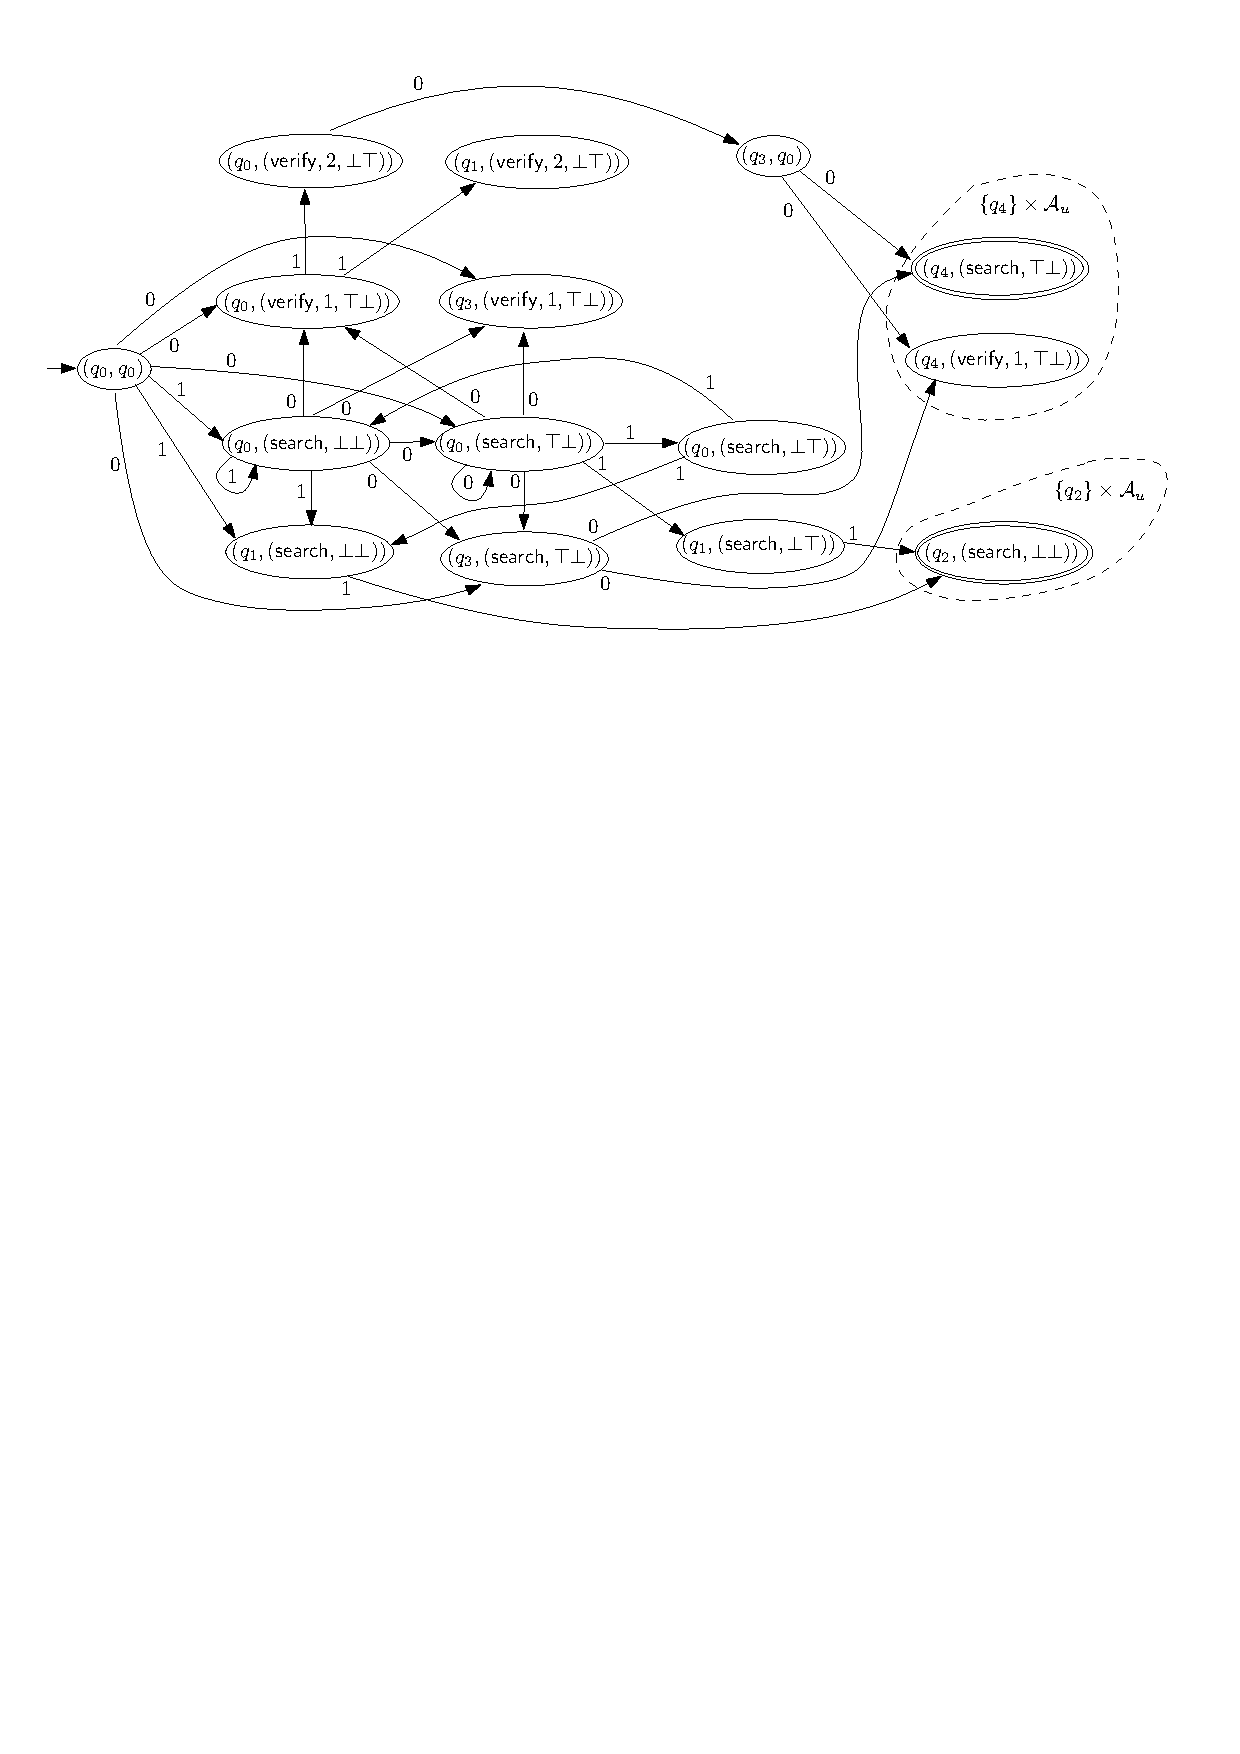
\includegraphics[scale=0.65]{constant-string-example.pdf}
\end{center}
\caption{The NFA $\cA_1 \times \cA_u$ for $u = 010$}\label{fig-cs-exmp}
\end{figure}
%

\def\refsecreplaceallcs{\ref{sec:replaceallcs}}
\section{Complexity analysis in Section~\protect\refsecreplaceallcs}
\label{sec:cs-complexity-full}

We provide a more detailed analysis of the complexity of the algorithm for the constant string case, described in Section~\ref{sec:replaceallcs}.
A summary of this argument already appears in Section~\ref{sec:replaceallcs}.

When constructing $G_{i+1}$ from $G_i$, suppose the two edges from $x$ to $y$ and $z$ respectively are currently removed, let the labels of the two edges be $({\sf l}, u)$ and $({\sf r}, u)$ respectively, then each element $(\cT, \cP)$ of $\cE_i(x)$ may be transformed into an element $(\cT', \cP')$ of $\cE_{i+1}(y)$ such that $|\cT'| = O(|u||\cT|)$, meanwhile, it may also be transformed into an element $(\cT'', \cP'')$ of $\cE_{i+1}(z)$ such that $\cT''$ has the same state space as $\cT$. Thus, for each source variable $x$, $\cE(x)$ contains at most exponentially many elements, and each of them may have a state space of at most exponential size. For instance, for a path from $x'$ to $x$ where the constant strings $u_1,\cdots, u_n$ occur in the labels of edges, an element $(\cT,\cP) \in \cE_0(x')$ may induce an element $(\cT', \cP')$ of $\cE(x)$ such that $|\cT'| \le |\cT| |u_1| \cdots |u_n|$, which is exponential in the worst case. 
%
To solve the nonemptiness problem of the intersection of all these regular constraints, the exponential space is sufficient. Consequently, in this case, we still obtain an EXPSPACE upper bound. 

Let us now consider the special situation that the $\rpleft$-length of $G_C$ is bounded by a constant $c$.
Since $\dmdidx(G_C) \le \lftlen(G_C)$, we know that $\dmdidx(G_C)$ is also bounded by $c$. Therefore, according to Proposition~\ref{prop-di}, there are at most polynomially different paths in $G_C$, we deduce that for each source variable $x$, $\cE(x)$ contains at most polynomially many elements. In addition, since the number of $\rpleft$-edges in each path is bounded by $c$, during the execution of the decision procedure, the number of times when $(\cT, \cP)$ of $\cE_i(x)$ may be transformed into an element $(\cT', \cP')$ of $\cE_{i+1}(y)$ such that $|\cT'| = O(|u||\cT|)$ is bounded by $c$.
Therefore, for each source variable $x$ and each element $(\cT'', \cP'')$ in $\cE(x)$,  $|\cT''|$ is at most polynomial in the size of $C$. We then conclude that for each source variable $x$, $\cE(x)$ corresponds to the intersection of polynomially many regular constraints such that each of them has a state space of polynomial size. Therefore, the nonemptiness of the intersection of all the regular constraints in $\cE(x)$ can be solved in polynomial space. In this situation, we obtain a PSPACE upper bound.


\def\refsecreplaceallre{\ref{sec:replaceallre}}
\section{Complexity analysis in Section~\protect\refsecreplaceallre}
\label{sec:re-complexity-full}

We provide a more detailed analysis of the complexity of the algorithm for the regular-expression case, described in Section~\ref{sec:replaceallre}.
A summary of this argument already appears in Section~\ref{sec:replaceallre}.

In each step of the reduction, suppose the two edges out of $x$ are currently removed, let the two edges be from $x$ to $y$ and $z$ and labeled by $({\sf l}, e)$ and $({\sf r}, e)$ respectively, then each element of $(\cT, \cP)$ of $\cE_i(x)$ may be transformed into an element $(\cT',\cP')$ of $\cE_{i+1}(y)$ such that $|\cT'| = |\cT| \cdot 2^{O(p(|e|))}$, meanwhile, it may also be transformed into an element $(\cT'',\cP'')$ of $\cE_{i+1}(y)$ such that $\cT''$ has the same state space as $\cT$. Thus, after the reduction, for each source variable $x$, $\cE(x)$ may contain exponentially many elements, and each of them may have a state space of exponential size, more precisely, if we start from a vertex $x$ without predecessors, with an element $(\cT,\cP)$ in $\cE_0(x)$, and go to a source variable $y$ through a path where $k$ edges have been traversed and removed, let $e_1,\cdots, e_k$ be the regular expressions occurring in the labels of these edges, then the resulting element in $\cE(y)$ has a state space of size $|\cT| \cdot 2^{O(p(|e_1|))} \cdot 2^{O(p(|e_2|))} \cdot \cdots \cdot 2^{O(p(|e_k|))}$ in the worst case. To solve the nonemptiness problem of the intersection of all these regular constraints, the exponential space is sufficient. Consequently, for the most general case of regular expressions, we still obtain a EXPSPACE upper bound. 

On the other hand, for the situation that the $\rpleft$-length of $G_C$ is at most one, we wan to show that the algorithm runs in polynomial space. Suppose the $\rpleft$-length of $G_C$ is at most one. Then the diamond index of $G_C$ is at most one as well. According to Proposition~\ref{prop-di}, there are only polynomially many paths in $G_C$. Nevertheless, for each source variable $x$, $\cE(x)$ may contain an element $(\cT,\cP)$ such that $|\cT|$ is exponential. Since $|\cP|$ may be exponential, $(\cT,\cP)$ may correspond to the intersection of exponentially many regular constraints. However, we can show that $|\cP|$ is at most polynomial, as a result of the fact that the $\rpleft$-length of $G_C$ is at most one. The arguments proceed as follows: Suppose two edges from $x$ to $y, z$ respectively are removed, and an element $(\cT', \cP')$ of $\cE_{i+1}(y)$ such that $|\cT'|$ is exponential and $|\cP'|$ is polynomial, is generated from an element of $(\cT, \cP)$ of $\cE_i(x)$. Then $y$ must be a source variable in $G_C$. Otherwise, there is an $\rpleft$-edge out of $y$ and the $\rpleft$-length of $G_C$ is at least two, a contradiction. Therefore, $y$ is a source variable in $G_C$, $(\cT', \cP')$  will not be used to generate the regular constraints for the other variables. In other words, $y$ is a source variable in $G_C$, and $(\cT', \cP') \in \cE(y)$ with $|\cP'|$ polynomial. We then conclude that for each source variable $x$, $|\cE(x)|$  is at most polynomial in the size of $C$ and for each element $(\cT, \cP) \in \cE(x)$, $|\cP|$ is polynomial in the size of $C$. Therefore, for each source variable $x$,  $\cE(x)$ corresponds to the intersection of polynomially many regular constraints, where each of them has a state space at most exponential size. To solve the nonemptiness of the intersection of these regular constraints, the polynomial space is sufficient. We obtain a PSPACE upper bound for the situation that the $\rpleft$-length of $G_C$ is at most one.


\def\refsecext{\ref{sec-ext}}
\section{Undecidability Proofs for Section~\protect\refsecext}
\label{sec:ext-undec-proofs}

\subsection{Proof of Theorem~\ref{thm-ext-int}}

\begin{proof}
	The basic idea of the reduction is to simulate the two polynomials $f(x_1,\cdots, x_n)$ and $g(x_1,\cdots, x_n)$, where $x_1,\cdots,x_n$ range over the set of natural numbers, with two $\strline[\concat,\replaceall]$ formulae $C_f, C_g$ over a unary alphabet $\{a\}$, with the output string variables $y_f, y_g$ respectively, and simulate the equality $f(x_1,\cdots, x_n) = g(x_1,\cdots, x_n)$ with the integer constraint $|y_f|=|y_g|$ (which is equivalent to $y_f = y_g$, since $y_f, y_g$ represent strings over the unary alphabet $\{a\}$). 
	
	A polynomial $f(x_1,\cdots, x_n)$ or $g(x_1,\cdots, x_n)$ where $x_1, \cdots, x_n$ range over the set of natural numbers, can be simulated by an $\strline[\concat,\replaceall]$ formula over an unary alphabet $\{a\}$ as follows: The natural numbers are represented by the strings over the alphabet $\{a\}$. A string variable is introduced for each subexpression of $f(x_1,\cdots, x_n)$. The numerical addition operator $+$ is simulated by the string operation $\concat$ 
	%\mat{$\concat$ is not part of $\strline[\replaceall]$, can it be simulated when the string alphabet is unary, or do we need two extra characters?}\zhilin{changed to $\strline[\concat,\replaceall]$.}
	and the multiplication operator $*$ is simulated by $\replaceall$. Since it is easy to figure out how the simulation proceeds, we will only use an example to illustrate it and omit the details here. Let us consider $f(x_1,x_2) = x_1^2 + 2 x_1 x_2 + 5$. By abusing the notation, we also use $x_1,x_2$ as string variables in the simulation. We will introduce a string variable for each subexpression in $f(x_1,x_2)$, namely the variables $y_{x_1^2}, y_{x_1x_2}, y_{2x_1x_2}, y_{x_1^2+2x_1x_2}, y_{f(x_1,x_2)}$. Then $f(x_1,x_2)$ is simulated by the $\strline[\concat,\replaceall]$ formula
	\[
	\begin{array} {l c l }
	C_f & \equiv & y_{x_1^2} = \replaceall(x_1,a, x_1)\ \wedge y_{x_1x_2} = \replaceall(x_1, a, x_2)\ \wedge \\
	& & y_{2x_1x_2} = \replaceall(aa, a, y_{x_1x_2})\ \wedge y_{x_1^2+2x_1x_2} = y_{x_1^2} \concat y_{2x_1x_2}\ \wedge  \\
	& & y_{f(x_1,x_2)}=y_{x_1^2+2x_1x_2} \concat a a a a a\ \wedge x_1 \in a^*\ \wedge x_2 \in a^*.
	\end{array}
	\]
	Then according to Proposition~\ref{prop-concat}, $C_f, C_g$ can be turned into equivalent $\strline[\replaceall]$ formula $C'_f, C'_g$ by introducing fresh letters.
	%\mat{But we may have to give up the unary alphabet?}\zhilin{yes, you are  right, it is fine.}
	
	Since $C'_f$ and $C'_g$ share only source variables $x_1,\cdots, x_n$, we know that $C'_f \wedge C'_g$ is still an $\strline[\replaceall]$ formula.
	From the construction of $C'_f, C'_g$, it is evident that for every pair of polynomials $f(x_1,\cdots, x_n)$ and $g(x_1,\cdots, x_n)$, $f(x_1,\cdots, x_n) = g(x_1,\cdots, x_n)$ has a solution in natural numbers iff $C'_f \wedge C'_g \wedge |y_f| = |y_g|$ is satisfiable. The proof is complete.
	%
	%%%%%%%%%%%%%%%%%%%%%%%%%%%%%%%%%%%%%%%%%%%%%%%%%%%%%%%%%%%
	%%%%%%%%%%%%%%%%%%%%%%%%%%%%%%%%%%%%%%%%%%%%%%%%%%%%%%%%%%%
	\hide{
		We shall reduce from the aforementioned version of the Hilbert tenth problem. For any polynomial with positive integral  $f(x_1, \cdots, x_n)$ where each coefficient is a positive, we can construct a (division-free) arithmetic circuit (AC) is a directed  acyclic graph with nodes labelled with constants from $\mathbb{Z}$, or with some indeterminates $X_1, \cdots, X_m$, or with the operators $+, -, *$. The nodes labelled with constants are called constant nodes, while those labelled with indeterminates are called input nodes. Both constant and input nodes do not have incoming edges. Internal nodes are those labelled with $+,-,*$. Output node is the one which does not have out-going edges. Without loss of generality we assume that each internal node has in-degree 2, and there is only one output node. Each node in the circuit represents a multivariate polynomial $\mathbb{Z}[X_1, \cdots, X_m]$. Vice verse, each polynomial $f\in \mathbb{Z}[X_1, \cdots, X_m]$ can be represented as an AC, and, if the polynomial has only positive (integral) coefficients, the corresponding AC does not contain nodes labelled by $-$ or negative constants.  
		
		We observe that, given an AC, one can construct an SL[$\concat, \replaceall$] formula over the alphabet $\Sigma=\{a\}$ as follows. Each node $n$ of the AC is associated with a string variable $x_n$. As a result, each input node of the AC labelled by $X_i$ (i.e., the indeterminate) corresponds to a  source variable.   
		\begin{itemize}
			\item For each internal node $n$ labelled by $+$, suppose that $n$ has two children nodes $n_l$ and $n_r$, we introduce a string constraint $x_n= x_{n_l}\concat x_{n_l}$.  
			
			\item For each internal node $n$ labelled by $*$, suppose that $n$ has two children nodes $n_l$ and $n_r$, we introduce a string constraint $x_n= \replaceall(x_{n_l}, a, x_{n_l})$.  		
		\end{itemize}
		Furthermore, we introduce, for each node $n$ labelled by a constant $c$, a regular constraint $x_n=a^c$. 
		
		It is straightforward to verify, according to the semantics of SL[$\concat, \replaceall$], that:
		\begin{itemize}
			\item for relational constraint $x_n= x_{n_l}\concat x_{n_l}$, $|x_n|= |x_{n_l}|+|x_{n_l}|$; 
			\item for relational constraint $x_n= \replaceall(x_{n_l}, a, x_{n_l})$,  $|x_n|= |x_{n_l}|\cdot |x_{n_l}|$; and 
			\item for regular $x_n=a^c$, $|x_n|=c$. 
		\end{itemize}
		
		It follows that for each polynomial $f(x_1, \cdots, x_m)$ with positive integral coefficients, we can construct a straight-line string constraint $\varphi_{f}\wedge\psi_g$ over $\Sigma=\{a\}$ with $y_f$ as the output variant and $y_1, \cdots, y_n$ as source variables such that
		$f(c_1, \cdots, c_m)=|y|$ and, for each $1\leq i\leq m$, $|y_i|= c_i$ (i.e., $y_i=a^{c_i}$).  
		
		Consequently, when given two polynomials $f(x_1, \cdots, x_m)$ and $g(x_1, \cdots, x_m)$, we have straight-line string constraints $\varphi_{f}\wedge \varphi_{g}\wedge \psi_{f}\wedge \psi_g$ with two distinguished two variables  $y_f$ and $y_g$ such that  
		\[\exists x_1, \cdots, x_m. f(x_1, \cdots, x_m)=g(x_1, \cdots, x_m)\mbox{ iff } |y_f|=|y_g|\wedge \varphi_{f}\wedge \varphi_{g}\wedge \psi_{f}\wedge \psi_g\mbox{ is satisfiable} \]
		
		Finally, note that any  SL[$\concat, \replaceall$] constraints can be transformed into SL[$\replaceall$] constraints, we obtain a reduction from the Hilbert's 10th problem to the satisfiability problem of  SL[$\replaceall$] with length constraints, which entail that the latter problem is undecidable. The proof is completed. 
	}
	%%%%%%%%%%%%%%%%%%%%%%%%%%%%%%%%%%%%%%%%%%%%%%%%%%%%%%%%%%%
	%%%%%%%%%%%%%%%%%%%%%%%%%%%%%%%%%%%%%%%%%%%%%%%%%%%%%%%%%%%
\end{proof}

\subsection{Undecidability of Depth-1 dependency graph}

A \emph{linear polynomial} (resp.\ quadratic polynomial) is a polynomial with degree at most one (resp.\ with degree at most two) where each coefficient is an integer. %of the form $a_0 + a_1x_1 + \cdots + a_n x_n$ (resp. a polynomial with degree at most two) where each coefficient $a_i\in \mathbb{Z}$  for $0 \leq i \leq n$. A quadratic polynomial

\begin{theorem}[\cite{ID04}]\label{thm-quad-eq}
	%	There exists some (fixed) $k$ such that no algorithm can solve Diophantine systems in the following form
	%	\[y_1F_1=G_1, t_1H_1=I_1, \cdots, t_kF_k = G_k, t_kH_k = I_k,\] 
	%
	%	where $F_i, G_i, H_i, I_i$ for $1\leq i\leq k$ are nonnegative linear polynomials over natural number variables  $s_1, \cdots, s_m$.
	The following problem is undecidable: Determine whether a system of equations of the following form has a solution in natural numbers, 
	\[
	\begin{array} {l l }
	A_i = B_i, & i =1, \cdots, k,\\
	y_iF_i=G_i \wedge y_i H_i = I_i, & i =1, \cdots, m, 
	\end{array}
	\] 
	%
	where $A_i, B_i, F_i, G_i$ are linear polynomials on the variables $x_1,\cdots, x_n$ (Note that each variable $y_i$ occurs in exactly two quadratic equations).
\end{theorem}

We can get a reduction from the problem in Theorem~\ref{thm-quad-eq} to the satisfiability of the extension of $\strline[\replaceall]$ with integer constraints as follows: For each monomial $y_i x_j$ in the quadratic polynomials, we use an $\strline[\replaceall]$ formula $z_{y_i x_j} = \replaceall(y_i, a, x_j)$ to simulate $y_i x_j$, where $z_{y_i x_j}$ are freshly introduced string variables. Since each equation $y_iF_i=G_i$ or $y_i H_i = I_i$ can be seen as a linear combination of the terms $y_i x_j$ and $x_j$ for $i \in [m]$ and $j \in [n]$, we can replace each variable $x_j$ with $|x_j|$, and each term $y_ix_j$ with $|z_{y_i x_j}|$,  thus transform them into the (linear) integer constraints $F'_i = G'_i$ or $H'_i = I'_i$. Similarly, after replacing each variable $x_j$ with $|x_j|$, we transform each equation $A_i= B_i$ into an integer constraint $A'_i = B'_i$. Therefore, we get a formula 
$$
\begin{array}{l c l }
\bigwedge \limits_{i \in [m], j \in [n]} z_{y_i x_j} = \replaceall(y_i, a, x_j) \wedge \bigwedge \limits_{i \in [m]} y_i \in a^*\ \wedge  \bigwedge \limits_{j \in [n]} x_j \in a^* \  \wedge\\
\hspace{2cm} \bigwedge \limits_{i \in [k]} A'_i = B'_i \wedge \bigwedge \limits_{i \in [m]} (F'_i = G'_i \wedge H'_i = I'_i),
\end{array}
$$
where the dependency graph of the $\strline[\replaceall]$ subformula is of depth at most one.

%%%%%%%%%%%%%%%%%%%%%%%%%%%%%%%%%%%%%%%%%%%%%%%%%
%%%%%%%%%%%%%%%%%%%%%%%%%%%%%%%%%%%%%%%%%%%%%%%%%
\hide{
	From this class of quadratic Diophantine equations, we can introduce string variables $x_1, \cdots, x_k$ and $y_1, \cdots, y_m$, together with relational string constraints 
	\[z_{i,j}=\replaceall(x_i, a, y_j)\]
	for $1\leq i\leq k$ and $1\leq j\leq m$. Note that, for each $i$,  $t_i F_i=G_i$ can be written as
	\begin{equation} \label{eq:dio}
	t_i\cdot \left(a_0+\sum_{j=1}^s a_j s_j\right) =  b_0+\sum_{j=1}^s b_j s_j
	\end{equation}
	where $a$'s and $b$'s are all natural numbers. Moreover, \eqref{eq:dio} holds iff 
	\[a_0\cdot |y_i|+ \sum_{j=1}^s a_j |z_{i,j}| =  b_0+ \sum_{j=1}^s b_j |x_j| \] 
	which is an integer constraint defined in Definition~\ref{def:intconst}. This entails that
}
%%%%%%%%%%%%%%%%%%%%%%%%%%%%%%%%%%%%%%%%%%%%%%%%%
%%%%%%%%%%%%%%%%%%%%%%%%%%%%%%%%%%%%%%%%%%%%%%%%%

\subsection{Undecidability of the character constraints}

\begin{proposition}\label{prop-ext-char}
	For the extension of $\strline[\replaceall]$ with character constraints, the satisfiability problem is undecidable. 
\end{proposition}

The arguments for Proposition~\ref{prop-ext-char} proceed as follows. Recall that in the proof of Theorem~\ref{thm-ext-int}, we get a formula $C_f \wedge C_g \wedge |y_f| = |y_g|$ such that $f(x_1,\cdots, x_n) = g(x_1,\cdots, x_n)$ has a solution in natural numbers iff $C_f \wedge C_g \wedge |y_f| = |y_g|$ is satisfiable. Let $\$ \neq a$. Suppose  $z_f = y_f \concat \$$, and $z_g = y_g \concat \$$. Then $|y_f| = |y_g|$ can be captured by $z_f[\mathfrak{n}] = \$[1] \wedge  z_g[\mathfrak{n}] = \$[1]$, where $\mathfrak{n}$ is a variable of type $\intnum$. More precisely, 
%
we have 
\begin{quote}
	\centering
	$C_f \wedge C_g \wedge |y_f|= |y_g|$ is satisfiable \\
	%
	iff \\
	%
	$C_f \wedge C_g \wedge z_f = y_f \concat \$ \wedge z_g = y_g \concat \$ \wedge z_f[\mathfrak{n}] = \$[1] \wedge  z_g[\mathfrak{n}] = \$[1]$ is satisfiable. 
\end{quote}
Therefore, we get a reduction from Hilbert's tenth problem to the satisfiability problem for the extension of $\strline[\replaceall]$ with character constraints. 

%For any two string variables $x,y$ on the unary alphabet $\{a\}$, let $x' = x \concat \$$ and $y' = y \concat \$$, then $|x| = |y|$ iff .
%
% $|x|=|y|$ iff $\exists n. x[n]=y[n]=\$$. 
%
%
%\begin{lemma}
%	For any two strings $x,y\in a^*\$$, $|x|=|y|$ iff $\exists n. x[n]=y[n]=\$$. 
%\end{lemma}
%
%As SL[$\replaceall$] with length constraints is undecidable, we conclude that 
%
%
%
%\tl{I am not satisfied with this as the quantifier is used}

\subsection{Undecidability of the $\indexof$ constraints}

\begin{proposition}\label{prop-indexof}
	For the extension of $\strline[\replaceall]$ with the $\indexof$ constraints, the satisfiability problem is undecidable. 
\end{proposition}

Proposition~\ref{prop-ext-char} follows from the following observation and Theorem~\ref{thm-ext-int}: For any two string variables $x,y$ over a unary alphabet, 
$1= \indexof(x,y)$ iff $x$ is a prefix of $y$. Therefore, $|x| = |y|$ iff $1=  \indexof(x,y) \wedge 1= \indexof(y,x)$. This implies that in the proof of Theorem~\ref{thm-ext-int}, we can replace $|y_f| = |y_g|$ with $1=\indexof(y_f, y_g) \wedge 1 = \indexof(y_g, y_f)$ and get a reduction from Hilbert's tenth problem to the satisfiability problem for the extension of $\strline[\replaceall]$ with the $\indexof$ constraints.
Note that $=$ can be simulated as a conjunction of $\leq$ and $\geq$.


%We have the following observation: 
%\begin{lemma}
%	For any two strings $x,y$ over $\{a\}$, $x=y$ iff $1=\indexof(x,y)=\indexof(y,x)$.  
%\end{lemma}
%
%It follows that 

%\subsection*{Further undecidability results}


\def\refsecreplaceallre{\ref{sec:replaceallre}}
\section{Examples in Section~\protect\refsecreplaceallre}

\begin{example}\label{exmp-pa-re}
	Let $e_0 = 0^*0 1(1^* + 0^*)$. Then $\cA_{0}$ and $\cA_{e_0}$ are illustrated in Figure~\ref{fig-pa-re}, where ${\sf sleft}$ and ${\sf slong}$ are the abbreviations of $\searchleft$ and $\searchlong$ respectively. Let us use the state $(\{q_{0,1}\}\{q_{0,0}\}, {\sf sleft}, \emptyset)$ to illustrate the construction. Since $\big(\delta_0(\{q_{0,1}\}, 0) \cup \delta_0(\{q_{0,0}\}, 0)\big) \cap F_0 = \{q_{0,1}\} \cap F_0 = \emptyset$, $\delta_0(\emptyset, 0) \cap F_0 = \emptyset$, and $\red(\delta_0(\{q_{0,1}\}, 0) \delta_0(\{q_{0,0}\}, 0))=\{q_{0,1}\}$, we deduce that the transition $((\{q_{0,1}\}\{q_{0,0}\}, {\sf sleft}, \emptyset), 0, (\{q_{0,1}\} \{q_{0,0}\}, {\sf sleft}, \emptyset)) \in \delta_{e_0}$. On the other hand, it is impossible to go from the state $(\{q_{0,1}\}\{q_{0,0}\}, {\sf sleft}, \emptyset)$ to the ``$\searchlong$'' mode. This is due to the fact that $\delta_0(\{q_{0,0}\}, 0)=\{q_{0,1}\} \subseteq \delta_0(\{q_{0,1}\},0)=\{q_{0,1}\}$. In addition, there are no $1$-transitions out of $(\{q_{0,1}\}\{q_{0,0}\}, {\sf sleft}, \emptyset)$. This is due to the fact that $\delta_0(\{q_{0,1}\}, 1) \cap F_0 = \{q_{0,2}, q_{0,3}\} \cap F_0 \neq \emptyset$.
	%
	\begin{figure}[htbp]
		\begin{center}
			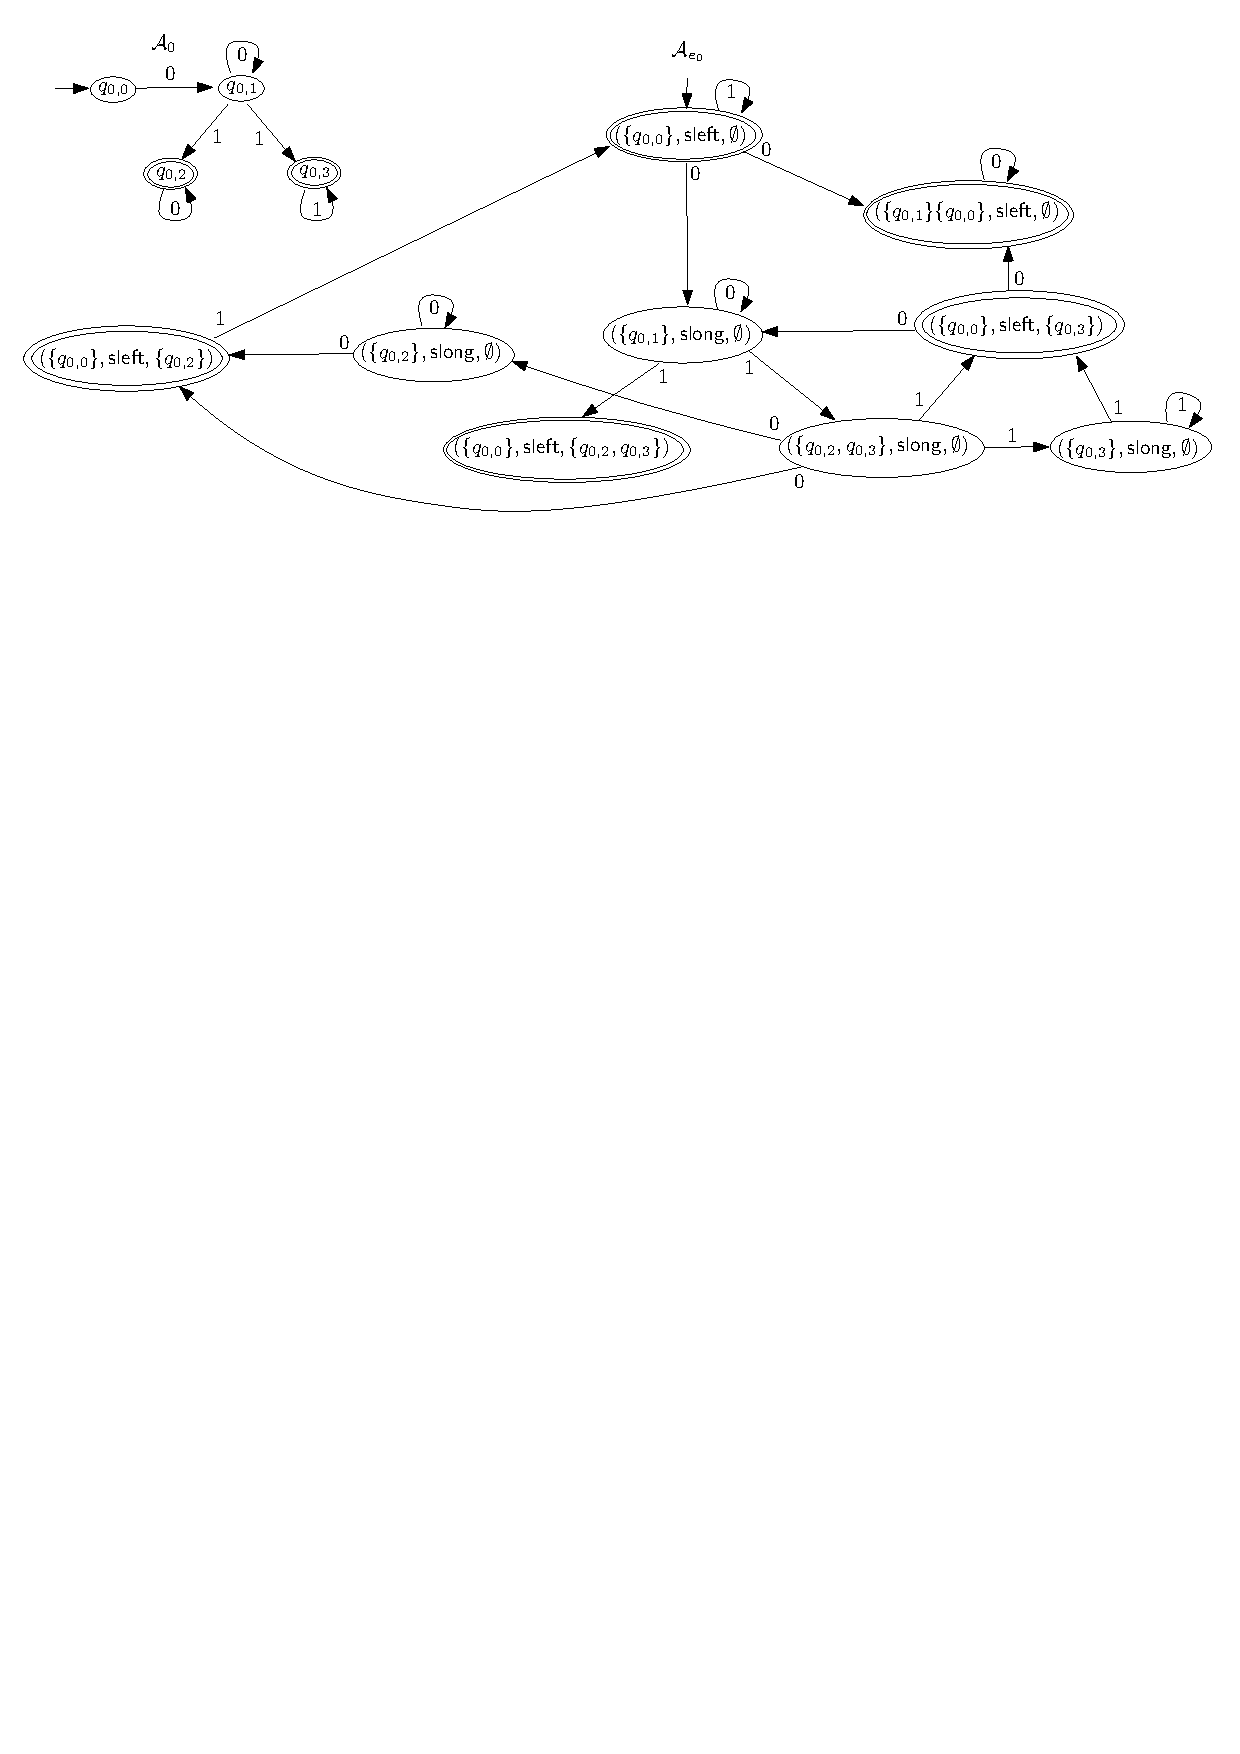
\includegraphics[scale=0.7]{regular-expression-example.pdf}
		\end{center}
		\caption{The NFA $\cA_0$ and $\cA_{e_0}$ for $e_0 = 0^*0 1(1^* + 0^*)$}\label{fig-pa-re}
	\end{figure} 
\end{example}

\begin{example}
	Let $C \equiv x = \replaceall(y, e_0, z) \wedge x \in e_1 \wedge y \in e_2 \wedge z \in e_3$, where $e_1,e_2,e_3$ are as in Example~\ref{exmp-sl} (cf. Figure~\ref{fig-sl-exmp}) and $e_0$ is as in Example~\ref{exmp-pa-re} (cf. Figure~\ref{fig-pa-re}). Suppose $T_z = \{(q_0, q_0), (q_1, q_2)\}$. Then the NFA $\cB_{\cA_1, e_0, T_z}$ is as illustrated in Figure~\ref{fig-re-exmp}, where the thick edges denote the added transitions. Let us use the state $(q_1, (\{q_{0,0}\}, \searchleft, \emptyset))$ to exemplify the construction. The transition $((q_1, (\{q_{0,0}\}, \searchleft, \emptyset)), 1, (q_2, (\{q_{0,0}\}, \searchleft, \emptyset)))$ is  in $\cA_1 \times \cA_{e_0}$. Since $\delta_0(q_{0,0}, 1) \cap F_0 = \emptyset$, this transition is not removed and is thus in $\cB_{\cA_1, e_0, T_z}$. On the other hand, since there are no $0$-transitions out of $q_1$ in $\cA_1$, there are no $0$-transitions from $(q_1, (\{q_{0,0}\}, \searchleft, \emptyset))$ to some state from $Q_{\searchleft}$ in $\cB_{\cA_1, e_0, T_z}$. 
	Moreover, because $((\{q_{0,0}\}, \searchleft, \emptyset), 0, (\{q_{0,1}\}, \searchlong, \emptyset)) \in \delta_{e_0}$ and $(q_1, q_2) \in T_z$, the transition $((q_1, (\{q_{0,0}\}, \searchleft, \emptyset)), 0, (q_1, (\{q_{0,1}\}, \searchlong, \emptyset)))$ is added. 
	One may also note that there are no 0-transitions from $(q_2, (\{q_{0,0}\}, \searchleft, \emptyset))$ to the state $(q_2, (\{q_{0,1}\}, \searchlong, \emptyset))$, because there are no pairs $(q2,-) \in T_z$.
	It is not hard to see that $010101 \in \Ll(\cA_2) \cap \Ll(\cB_{\cA_1, e_0, T_z})$. In addition, $10 \in \Ll(\cA_3) \cap \Ll(\cA_1(q_0,q_0)) \cap \Ll(\cA_1(q_1,q_2))$. Let $y$ be $010101$ and $z$ be $10$. Then $x$ takes the value $\replaceall(010101, e_0, 10)=10 \cdot \replaceall(101, e_0, 10)=10110$, which is accepted by $\cA_1$. Therefore, $C$ is satisfiable.
	\begin{figure}[htbp]
		\begin{center}
			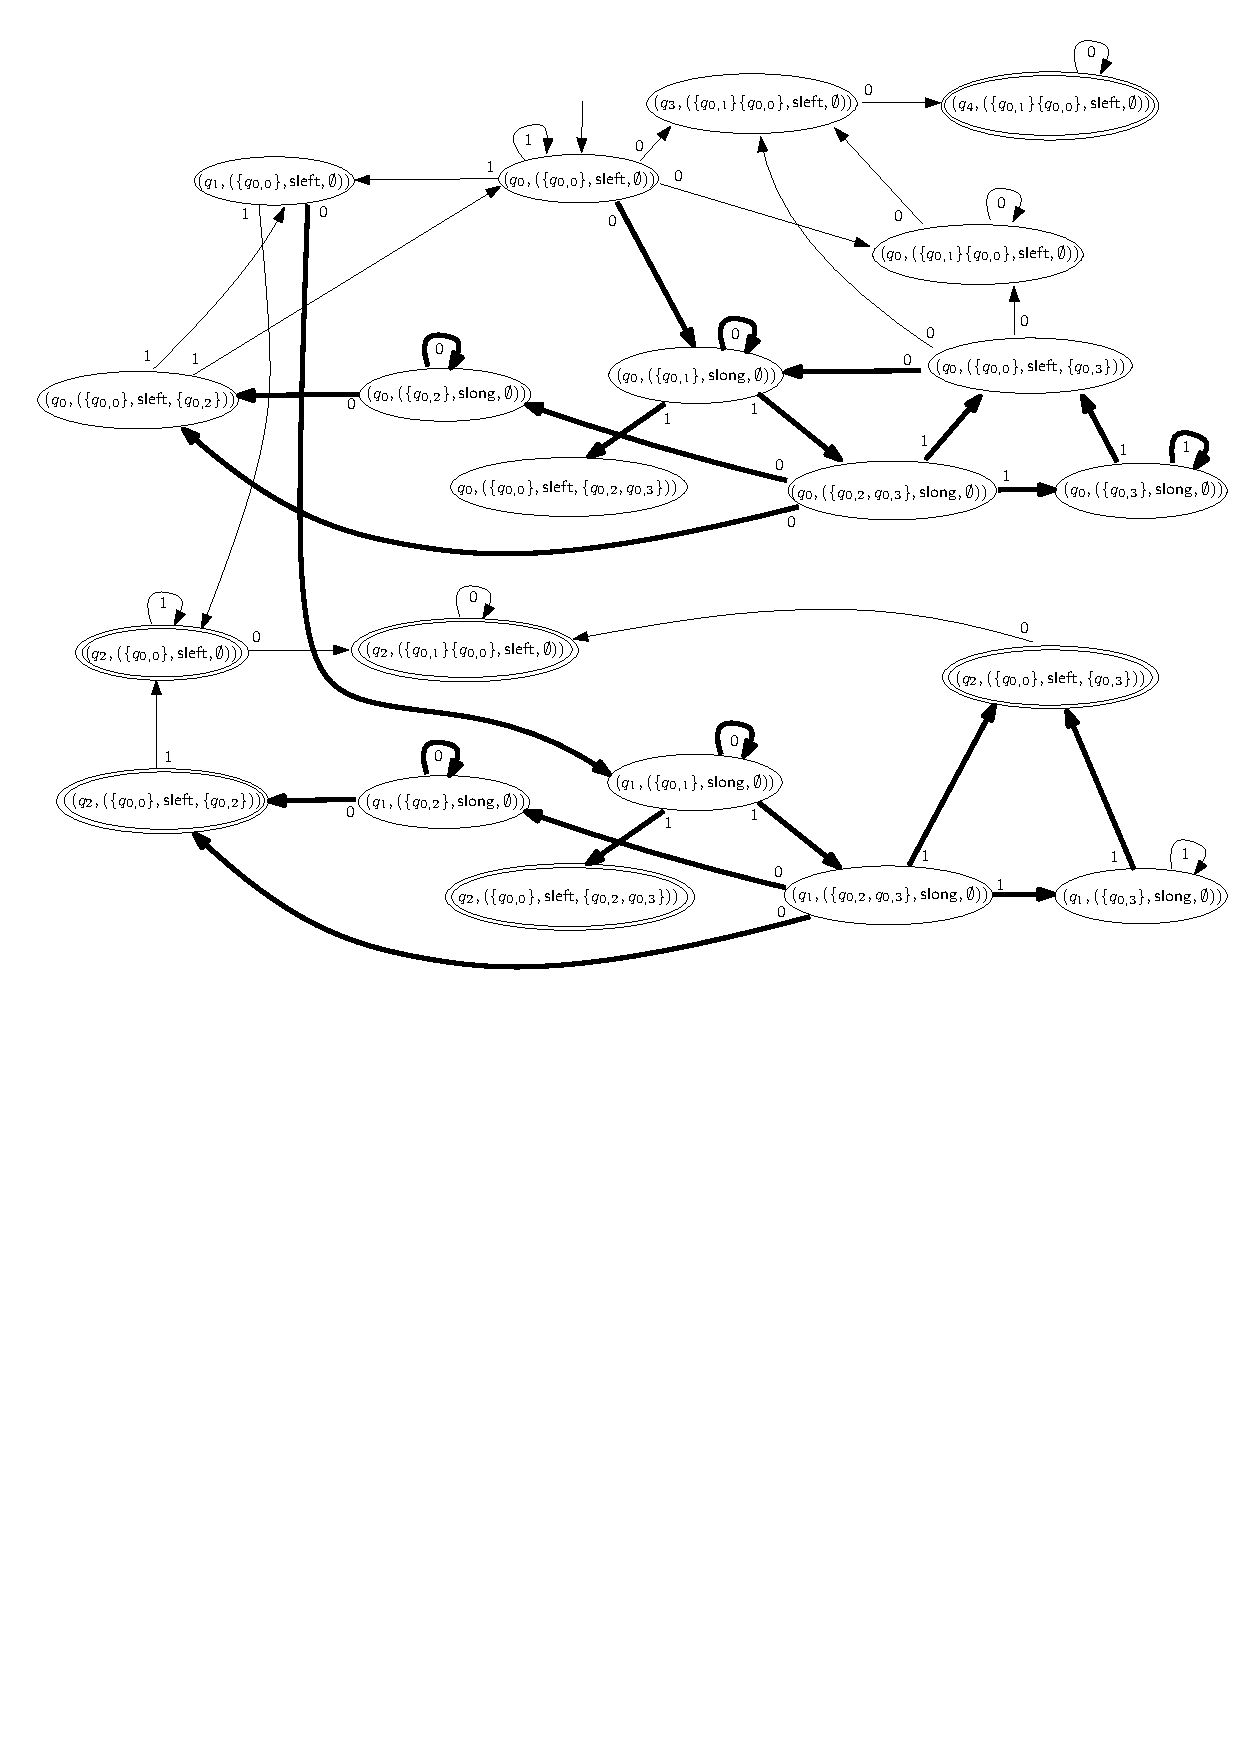
\includegraphics[scale=0.68]{regular-expression-example-2.pdf}
		\end{center}
		\caption{The NFA $\cB_{\cA_1, e_0, T_z}$}\label{fig-re-exmp}
	\end{figure} 
\end{example}





\end{document}
